\documentclass[12pt, a4paper,twoside]{tesi_upf}

%CODIFICATION
\usepackage[latin1]{inputenc}
%LENGUAGE
\usepackage[catalan,english]{babel}
%ONLY TO OBTAIN MARK BANK INDEX INDICATION A4
\usepackage[cam,a4,center,frame]{crop}
%INCLUDE GRAPHICS AND THE LOGO OF THE UPF
\usepackage{graphicx}
%FONTS TIMES OR GARAMOND, 
\usepackage{times}
%\usepackage{garamond}
%WITHOUT HEADINGS: NO MODIFICATION
\pagestyle{plain}
%FOR THE INDEX OF SUBJECTS
\usepackage{makeidx}
\makeindex
%BIBLIOGRAPHY STYLE
\bibliographystyle{unsrt}
%SELECT LANGUAGE
\selectlanguage{catalan}
 
\usepackage{cite}
% Equations
\usepackage{amsmath,amssymb,amsfonts}

% Hyperreferences
\usepackage{url}
%\usepackage{hyperref}

\usepackage{subfigure}

\usepackage{graphicx} 	  %% The graphicx package provides the includegraphics command.
\usepackage{amssymb} 	%% The amssymb package provides various useful mathematical symbols

\usepackage{color}
\usepackage{amsmath}
\usepackage{mathtools}
\usepackage{fullpage}
\usepackage{algorithmic}
\DeclareMathOperator*{\argmin}{argmin}
\DeclareMathOperator*{\argmax}{argmax}
\algsetup{linenosize=\small}
\usepackage[table,xcdraw]{xcolor}
\usepackage{multirow}
\usepackage[super]{nth}
\usepackage{graphicx,adjustbox}
\usepackage{comment}
\usepackage{setspace}
\usepackage{textcomp}
\usepackage{xspace}
\usepackage{siunitx}
\usepackage{epsfig}
\usepackage{epstopdf}
\usepackage{soul}
\usepackage{tablefootnote}
\DeclareMathOperator{\E}{\mathbb{E}} % Expectation Symbol
\usepackage[linesnumbered,ruled]{algorithm2e}
\usepackage{booktabs}
\usepackage[normalem]{ulem}
\usepackage{footnote}
\usepackage[misc,geometry]{ifsym} 
\bibliographystyle{abbrvnat}
\makesavenoteenv{tabular}

\usepackage[edges]{forest}
\usetikzlibrary{shadows,arrows.meta}
\usepackage{tcolorbox}
%Defining the styles used in trees
%Note that the fill colour is not defined here.
\tikzset{parent/.style={align=center,text width=2cm,rounded corners=2pt},
	child/.style={align=center,text width=6.5cm,rounded corners=6pt},
	grandchild/.style={align=left, text width=10cm}
}

\hyphenation{Re-use}

\usepackage{pdfpages}

%THE TABLE OF CONTENTS IS TITLE CONTENTS
%\addto\captionscatalan
\renewcommand{\contentsname}{\Large \sffamily Table of contents}

%ADD YOUR DATA
\title{Towards Spatial Reuse in Future Wireless Local Area Networks: a Sequential Learning Approach}

%\subtitle{The subtitle of the thesis: Required}
\author{Francesc Wilhelmi Roca}
\thyear{2020}
\department{of Information and Communication Technologies}
\supervisor{Boris Bellalta, Cristina Cano \& Anders Jonsson}

\begin{document}

\frontmatter
\maketitle
\cleardoublepage

%%%%%% Dedication
\noindent Write here your dedication
\cleardoublepage
%%%%%% End dedication

%%%%%% Thanks
\section*{\Large \sffamily  Acknowledgments}
%\noindent {\Large \sffamily Acknowledgments} 
This work has been partially supported by grants MDM-2015-0502, 2017-SGR-11888, by WINDMAL PGC2018-099959-B-I00 (MCIU/AEI/FEDER,UE), and by a Gift from the Cisco University Research Program (CG\#890107) Fund.%, and by SPOTS project (RTI2018-095438-A-I00) funded by the Spanish Ministry of Science, Innovation and Universities.
\cleardoublepage
%%%%%% End of thanks

%ABSTRACT IN TWO LEGUAGES.
\selectlanguage{english}
\section*{\Large \sffamily Abstract}
The Spatial Reuse (SR) operation is gaining momentum in the latest IEEE 802.11 family of standards due to the overwhelming requirements posed by next-generation wireless networks. In particular, the increasing traffic capacity and the number of concurrent devices compromise the efficiency of increasingly dense Wireless Local Area Networks (WLANs) and throw into question their decentralized nature. The SR operation, initially introduced by the IEEE 802.11ax-2021 amendment and further studied in IEEE 802.11be-2024, aims to increase the number of concurrent transmissions in an Overlapping Basic Service Set (OBSS), thus improving spectral efficiency. SR was initially defined as a distributed mechanism, but it is evolving towards coordinated schemes where different BSSs cooperate. Nevertheless, coordination entails communication and synchronization overhead, which impact the performance of WLANs that remains unknown. Moreover, the coordinated scheme is incompatible with devices using previous IEEE 802.11 versions, potentially leading to degrading the performance of legacy networks. For those reasons, in this thesis, we assess the viability of decentralized mechanisms for SR, and thoroughly examine the main impediments and shortcomings that may result from it. We aim to shed light on the future shape of WLANs concerning SR optimization and whether their decentralized nature should be kept or preferable to evolve towards coordinated and centralized settings. Given the challenges posed by the decentralized SR problem, we focus on Artificial Intelligence (AI) and propose using a class of sequential learning-based methods, namely Multi-Armed Bandits (MABs). The MAB setting suits the decentralized SR problem because it addresses the uncertainty caused by the concurrent operation of multiple devices (i.e., multi-player setting) and the lack of information resulting from it. MABs can potentially overcome the complex and varying spatial interactions among devices that result from modifying their sensitivity and transmit power. Nevertheless, the application of multi-agent sequential learning to communications raises several concerns that may compromise network devices' performance (definition of joint goals, time-horizon convergence, scalability aspects, non-stationarity, etc.). Our analysis of decentralized SR encompasses an in-depth study of the SR technology, infrastructure aspects for AI-enabled networking, and the suitability of the sequential learning approach.

\vspace*{\fill}
\pagebreak

\section*{\Large \sffamily Resum}
\textcolor{red}{To be written once the English version is definitive.}

\vspace*{\fill}

\cleardoublepage
%END OF ABSTRACT

\section*{\Large \sffamily List of Publications}

\begin{enumerate}
	\item Wilhelmi, F., Bellalta, B., Cano, C., \& Jonsson, A. (2017, October). \textit{Implications of decentralized Q-learning resource allocation in wireless networks}. In 2017 IEEE 28th annual international symposium on personal, indoor, and mobile radio communications (PIMRC) (pp. 1-5). IEEE.
	\item Wilhelmi, F., Cano, C., Neu, G., Bellalta, B., Jonsson, A., \& Barrachina-Mu�oz, S. (2019). \textit{Collaborative spatial reuse in wireless networks via selfish multi-armed bandits.} Ad Hoc Networks, 88, 129-141.
	\item Wilhelmi Roca, F., Barrachina Mu�oz, S., Bellalta, B., Cano Sand�n, C., Jonsson, A., \& Neu, G. (2019). \textit{Potential and pitfalls of multi-armed bandits for decentralized spatial reuse in WLANs.} Journal of Network and Computer Applications, 2019, 127.
	\item Barrachina-Mu�oz, S., Wilhelmi, F., Selinis, I., \& Bellalta, B. (2019, April). \textit{Komondor: a wireless network simulator for next-generation high-density WLANs.} In 2019 Wireless Days (WD) (pp. 1-8). IEEE.
	\item Wilhelmi, F., Mu�oz, S. B., Cano, C., Selinis, I., \& Bellalta, B. (2019). \textit{Spatial Reuse in IEEE 802.11 ax WLANs.} arXiv preprint arXiv:1907.04141.
	\item Wilhelmi, F., Barrachina-Mu�oz, S., \& Bellalta, B. (2019, October). \textit{On the Performance of the Spatial Reuse Operation in IEEE 802.11 ax WLANs.} In 2019 IEEE Conference on Standards for Communications and Networking (CSCN) (pp. 1-6). IEEE.
	\item Wilhelmi, F., Barrachina-Munoz, S., Bellalta, B., Cano, C., Jonsson, A., \& Ram, V. (2020). \textit{A Flexible Machine-Learning-Aware Architecture for Future WLANs. IEEE Communications Magazine, 58(3), 25-31.}	
	\item Wilhelmi, F., Carrascosa, M., Cano, C., Ram, V., \& Bellalta, B. (2020). \textit{Usage of Network Simulators in Machine-Learning-Assisted 5G/6G Networks.}
\end{enumerate}
%Decentralized learning with cost in IEEE 802.11 WLANs
%Survey MABs for communications

%%PREFACE. 
%{\bf Preface}

\cleardoublepage
%END OF PREFACE

%TABLE OF CONTENTS: REQUIRED
\tableofcontents

%\noindent{\bfseries{\huge Contents}\hfill Page No.\vspace \bigskipamount \par }
%\contentsline {chapter}{\numberline {1}INTRODUCTION}{1}
%\contentsline {section}{\numberline {1.1}Motivation}{1}
%\contentsline {section}{\numberline {1.2}Contributions}{2}
%\contentsline {subsection}{\numberline {1.2.1}Contributions to the Research Community}{2}
%\contentsline {subsection}{\numberline {1.2.2}Contributions to Standardization}{3}
%\contentsline {section}{\numberline {1.3}Document Structure}{3}

%\contentsline {chapter}{\numberline {2}SPATIAL REUSE IN IEEE 802.11 WLANS}{5}
%\contentsline {section}{\numberline {2.1}Related Work}{2}
%\contentsline {section}{\numberline {2.2}Spatial Reuse in IEEE 802.11ax}{2}
%\contentsline {subsection}{\numberline {2.2.1}OBSS/PD-based Spatial Reuse}{3}
%\contentsline {subsection}{\numberline {2.2.1}Parametrized Spatial Reuse}{3}
%\contentsline {section}{\numberline {2.3}Spatial Reuse in IEEE 802.11be}{2}

%\contentsline {chapter}{\numberline {3}MACHINE LEARNING IN WLANS}{5}
%\contentsline {section}{\numberline {3.1}Computation Paradigms}{2}
%\contentsline {section}{\numberline {3.2}Architectural Aspects of Machine-Learning-Aware Networks}{2}
%\contentsline {section}{\numberline {3.3}Multi-Armed Bandits in Communications}{2}
%\contentsline {section}{\numberline {3.4}Multi-Armed Bandits for Decentralized Spatial Reuse: Between ML and Game Theory}{2}

%\contentsline {chapter}{\numberline {4}METHODOLOGY AND ENABLERS}{5}
%\contentsline {section}{\numberline {4.1}Spatial Reuse through Continuous Time Markov Networks}{2}
%\contentsline {subsection}{\numberline {4.1.1}IEEE 802.11ax OBSS/PD-based Spatial Reuse}{3}
%\contentsline {subsection}{\numberline {4.1.2}IEEE 802.11be Coordinated Spatial Reuse}{3}
%\contentsline {section}{\numberline {4.2}Simulation of Sequential Learning and Spatial Reuse}{2}
%\contentsline {subsection}{\numberline {4.2.1}Spatial Reuse Implementation}{3}
%\contentsline {subsection}{\numberline {4.2.2}Agents-based implementation}{3}

%\contentsline {chapter}{\numberline {5}MAIN FINDINGS}{5}

%\contentsline {chapter}{\numberline {6}CONCLUDING REMARKS}{5}

%\contentsline {chapter}{\numberline {7}LIST OF PUBLICATIONS}{5}

%lIST OF FIGURES; ONLY IF THERE ARE FIGURES
%\listoffigures
%TO APPER THE LIST OF FIGURES IN THE TABLE OF CONTENTS 
%\addcontentsline{toc}{chapter}{List of figures}

%LIST OF TABLES; ONLY IF THERE ARE TABLES
%\listoftables
%TO APPEAR THE LIST OF TABLES IN THE TABLE OF CONTENTS
%\addcontentsline{toc}{chapter}{List of tables}

%START THE TEXT
\mainmatter

%%%%%%%%%%%%%%%%%
% INTRODUCTION
%%%%%%%%%%%%%%%%%
\chapter{Introduction}

%A la intro, deixa clar que SR �s part de WIFI, per� que la tesi aporta cosa m�s enll� d'aquesta tecnologia.
%
%Resum: M'agrada molt el que has escrit, per� intentaria separar els conceptes de la tecnologia. 
% - Pq SR �s important, 
% - Pq necessitem fer servir ML / AI per trobar solucions que sense ML / AI no s�n possibles. 
% Aix� es pot fer amb un parell de par�grafs al principi de tot, i despr�s ja pots entrar en WIFI justificant la rellev�ncia de WIFI, per� sobretot els challenge que representa que tingui una gesti� totalment 'dencentralitzada' per a poder implementar t�cniques com SR.

\section{Motivation}
% Introduction to IEEE 802.11 WLANs 
The Institute of Electrical and Electronics Engineers (IEEE) 802.11 family of protocols for wireless local area networks (WLANs) was first released in 1997 as a novel solution for physical (PHY) and medium access control (MAC) layers. Since that date, the standard has evolved to sustain the increasing user requirements in terms of capacity, load, and coverage, as well as serve for different purposes (e.g., mesh networking, security-enhanced communications, channel measurement, etc.). The set of new and improved capabilities have been captured along the time in the plethora of amendments that followed the initial 802.11-1997 standard (e.g., 802.11b, 802.11g, 802.11h, etc.). 

% Next-generation of IEEE 802.11 WLAN standards
Looking ahead, the next generation of WLAN standards is expected to revolutionize the telecommunications and converge along with 5G systems and beyond to expand to multiple domains, such as light communications (IEEE 802.11bb), Internet of Things (IEEE 802.11ah), vehicle-to-everything (IEEE 802.11bd), or next-generation positioning (IEEE 802.11az). One of the most influential amendments is the IEEE 802.11ax-2021 (11ax) amendment for High Efficiency (HE) WLANs \cite{bellalta2016ieee, deng2014ieee, khorov2018tutorial}, which primary goal is to enhance network efficiency in ultra-dense deployments to grant high capacity (up to 10 Gbps). In particular, the 11ax (commercially known as Wi-Fi 6) includes a set of unprecedented techniques, such as Orthogonal Frequency Division Multiple Access (OFDMA), Downlink/Uplink Multi-User Multiple-Input-Multiple-Output (DL/UL MU-MIMO), and Spatial Reuse (SR), for addressing the broad range of issues arisen from high-density scenarios \cite{merlin2015tgax}.

% What is SR and what it is aimed to solve
This thesis focuses on the SR operation, which started with IEEE 802.11ax and is now evolving in the IEEE 802.11be. SR aims to enhance spectral efficiency by increasing the number of parallel transmissions in high-dense deployments. To this end, SR proposes a mechanism to ignore transmissions whose source is a device belonging to a different Basic Service Sets (aka inter-BSS transmissions). As a result, a less restrictive carrier sense threshold is used for inter-BSS transmissions, referred to as Overlapping BSS Packet Detect (OBSS/PD) threshold. To promote fairness, SR also incorporates a mechanism that limits the transmit power of the new transmissions resulting from a less restrictive OBSS/PD threshold (so that primary transmissions are not affected). Table \ref{table:effects_sr} summarizes the potential effects and implications of adjusting the sensitivity threshold and the transmit power in WLANs.

\begin{table*}[ht!]
\caption{Effects and implications of adjusting the sensitivity threshold and the transmit power in IEEE 802.11 WLANs.}
\label{table:effects_sr}
	\resizebox{\textwidth}{!}{%
		\begin{tabular}{|c|c|c|c|c|c|}
		\hline
		& \textbf{Data rate} & \textbf{\begin{tabular}[c]{@{}c@{}}Channel access\\ probability\end{tabular}} & \textbf{\begin{tabular}[c]{@{}c@{}}Generate starvation\\ probability\end{tabular}} & \textbf{\begin{tabular}[c]{@{}c@{}}Hidden-node\\ probability\end{tabular}} & \textbf{\begin{tabular}[c]{@{}c@{}}Exposed-node\\ probability\end{tabular}} \\ \hline
		\textbf{Sensitivity $\uparrow$} & - & $\uparrow$ & $\uparrow$ & $\uparrow$ & $\downarrow$ \\ \hline
		\textbf{Tx. power $\uparrow$} & $\uparrow$ & - & $\uparrow$ & $\downarrow$  & $\uparrow$ \\ \hline
	\end{tabular}}
\end{table*}

% Role of AI
To address the underlying complexity of SR, we study the application of Artificial Intelligence (AI) mechanisms for automatically adjusting both the sensitivity and the transmit power of wireless devices. AI is gaining momentum in telecommunications -- it is in fact expected to be pervasively included as part of the network operation in 6G systems \cite{strinati20196g, shafin2020artificial, giordani2020toward} -- due to its ability to exploit complex characteristics from data, thus allowing to solve problems that are hard to solve by hand-programming.

\section{Contributions}

\subsection{Contributions to the Research Community}
% Proposal to use ML for SR
In light of the importance of SR for future wireless networks and the current evolution of communications towards AI-enabled systems, in this thesis, we study the potential application of Machine Learning (ML) for addressing the challenges raised by SR. In particular, we aim to shed light on the potential gains of SR and devise its intersection with AI. The contributions of this thesis are summarized next:
\begin{enumerate}
	\item We study state-of-the-art solutions for improving spectral efficiency in wireless networks. In particular, we focus on methods based on sensitivity adjustment and power control. Then, we narrow the scope to IEEE 802.11-based SR solutions, mostly oriented to 11ax systems.
	\item We provide an in-depth overview of the SR operation included in the IEEE 802.11ax amendment. Besides, we devise the potential evolution path of the SR technology in IEEE 802.11be and beyond.
	\item We analytically model the SR operation and study the new kind of inter-networks interactions resulting from it. Thanks to the model, we can deeply understand the implications of applying SR.
	\item We provide a simulation-based implementation of the SR operation, from which we extract results of its performance gains in future dense WLANs. The presented simulation tool allows for the inclusion of new blocks cost-effectively and serves to devise the potential of new technologies such as coordinated spatial reuse. Besides, our simulator allows characterizing high-density deployments in affordable simulation time. 
	\item We propose several ML-based solutions to address the SR problem in decentralized WLAN deployments. The simulation-based implementation of these methods allows us to study the performance gains compared to default carrier sensing approaches. In particular, we show that the concurrent learning operation may lead to suboptimal configurations in aggregate performance. Nevertheless, we also show that decentralized learning can help to mitigate unfairness in wireless networks when cooperation is enabled.
	\item We study implications that decentralized ML solutions have on the operation of WLANs. In particular, we focus on the game-theoretic setting caused by the concurrent devices attempting to learn the best SR configuration. Besides, we delve into practical implementation aspects related to the communication limitations for cooperative approaches, the amount of information available for learning, and the dynamism of wireless networks.
	\item We delve into architectural aspects to enable future ML-aware networks. Because of the promising performance gains that ML can provide to networking systems, its actual integration is currently a topic that is attracting a lot of attention. Special emphasis is being put on data handling and flexible interfaces, which are meant to address the issues related to data storage, data exchange, and data processing.
\end{enumerate}

\subsection{Contributions to Standardization}
Apart from the contributions related to the research on SR and AI, we have participated in many standardization initiatives. Specifically, the output contributions in the context of International Telecommunications Union Telecommunication Standardization Sector (ITU-T) are as follows:
\begin{enumerate}
	\item As part of the ITU's architectural framework for ML-enabled networks, we developed a specification on an isolated domain for training, testing, and evaluating ML models for communications.
    \item We contributed to the group through the following topics: \emph{i)} considerations when applying ML in heterogeneous environments in which both intelligent and non-intelligent (legacy) devices coexist, \emph{ii)} practical usage of simulators for generating synthetic data sets that serve for training ML models, and \emph{iii)} a use-case realization of the ITU's ML-aware architecture for IEEE 802.11 WLANs.
	\item We provided a data set to address the problem of channel bonding in future WLANs through ML.\footnote{All the details on the problem statement can be found at \url{https://www.upf.edu/web/wnrg/ai_challenge}} This data set has been developed in the context of the ITU-T AI Challenge - 2020, which aims to boost innovation in the integration of AI/ML into 5G networks and beyond.
\end{enumerate}

\section{Document Structure}
% Structure
This thesis is a compendium of articles resulting from the research activity on ML's application to address SR in IEEE 802.11 WLANs. We refer to the publications on page ix as Paper~\#1 through Paper \#8. Besides the list of publications (attached at the end of this document), a monograph is provided to introduce the research topic and give some background on the same. This document is structured as follows. Chapter \ref{chapter2} surveys SR techniques in wireless networks, overviews the IEEE 802.11ax SR operation, and discusses the evolution of SR in future amendments. Chapter \ref{chapter3} provides insights on the intersection between ML and wireless communications, including architectural aspects and state-of-the-art applications. Then, the SR problem is formulated through Multi-Armed Bandits. Chapter \ref{chapter4} introduces the analytical and simulation tools used for performance evaluation. The main finding of this thesis are summarized in Chapter \ref{chapter5}, and concluding remarks are provided in Chapter \ref{chapter6}.
 
%%%%%%%%%%%%%%%%%
% TECHNOLOGY
%%%%%%%%%%%%%%%%%
\chapter{Spatial Reuse in IEEE 802.11 WLANs}
\label{chapter2}

In this Chapter, we describe the SR operation and survey the related work, ranging from solutions for sensitivity and transmit power adjustment in wireless networks, to specific IEEE 802.11 mechanisms. Then, we overview the IEEE 802.11ax SR operation and discuss the next steps being taken by the Task Group 802.11be (TGbe) to make this technology evolve.

\section{Related Work}

Improving medium utilization through SR has been extensively studied for sensitivity and transmit power adjustment in different domains such as multi-hop networks \cite{kim2006improving, alawieh2009improving}, cellular networks \cite{zhang2017survey}, and IEEE 802.11 WLANs \cite{thorpe2014survey}. SR can be realized through beamforming/null-steering \cite{vilzmann2006survey}, OFDMA-based multi-user scheduling \cite{yaacoub2011survey}, MU-MIMO transmissions \cite{liao2014mu}, sensitivity adjustment \cite{thorpe2014survey}, and transmission power control \cite{xu2015robust}. In this thesis, we focus on sensitivity and transmit power adjustment, which does not require additional infrastructure and promises substantial performance gains concerning the lack of efficiency of the current IEEE 802.11 channel sharing methods \cite{alawieh2009improving}. 

Sensitivity and transmit power adjustment has been applied in different manners to address multiple problems (improve capacity, boost fairness, save energy, etc.). Figure�\ref{fig:sr_survey} shows a categorization of these SR techniques according to the optimization goal and their implementation. In particular, we find CS/CCA adaptation mechanisms, power control, and joint CS/CCA adaptation and power control. While some of the works focus their attention on modeling and analyzing the effects of tuning sensitivity and transmit power in wireless networks, others provide different optimization mechanisms. Iterative methods have been typically applied to decentralized and varying deployments (see, for instance, the work in \cite{fang2017intelligent}). Apart from that, pre-defined solutions are based on a preliminary analysis of the implications of sensitivity adjustment and power control in particular network settings. In \cite{murakami2015improving}, for instance, the authors provide a Carrier Sense Threshold (CST) adaptation mechanism based on the location of APs. In particular, a position-CST table is derived from a preliminary analysis of the conditions that allow APs to transmit concurrently without suffering losses. Finally, global solutions are provided for deployments that can be fully controlled at a single point (availability of complete information or coordinated setting). This is the case of the work in \cite{liang2019towards}, where DL is used to maximize the sum-rate under Quality of Service (QoS) constraints in multi-user power control.

\begin{figure}[ht!]
	\centering
	\resizebox{.9\textwidth}{!}{\begin{forest}
		forked edges,
		for tree={
			grow'=0,
			draw,
			align=c,
			font=\sffamily,
			rounded corners,
		},
		highlight/.style={
			thick,
			font=\sffamily\bfseries
		}
		[{Spatial Reuse\\Techniques}, highlight, fill=gray!30
		[{CS/CCA adaptation}, for tree={child, fill=green!30}
		[{Analysis: \cite{zhu2008optimal, ma2009optimizing, deng2004tuning, yang2005physical, ma2005stochastic, tayamon2015analysis,jamil2014improving}},font=\fontsize{12}{0}\selectfont]
		[{Iterative methods: \cite{zhu2006adaptive,haghani2010adaptive,thorpe2011ieee802,fu2012effective,kim2013iterative,yin2019learning,schmidt2011advanced,park2009noncooperative,smith2015dynamic,ropitault2017etp, selinis2018control, ropitault2018evaluation, valkanis2019ieee}},font=\fontsize{12}{0}\selectfont]
		[{Pre-defined solutions: \cite{murakami2015improving, oni2015ap}},font=\fontsize{12}{0}\selectfont]
		[{Global solutions: \cite{nakahira2014centralized, afifi2016throughput}},font=\fontsize{12}{0}\selectfont]
		]
		[{Power control}, for tree={child, fill=yellow!20}
		[{Iterative methods: \cite{li2014energy,chevillat2005dynamic,fang2017intelligent,islam2019dynamic,chaves2014adaptive,gandarillas2014dynamic}},font=\fontsize{12}{0}\selectfont]
		[{Pre-defined solutions: \cite{chang2007power,tang2011improving, kim2014distributed,shimizu2019joint,ebert2000energy,lei2015performance}},font=\fontsize{12}{0}\selectfont]
		[{Global solutions: \cite{li2011achieving,oteri2013advanced,tang2014joint,amiri2019reinforcement,liang2019towards}},font=\fontsize{12}{0}\selectfont]
		]
		[{Joint CS/CCA adaptation\\ \& Power control}, for tree={child, fill=cyan!30}
		[{Analysis: \cite{yamamoto2017analysis,iwata2019analysis,fuemmeler2006selecting}},font=\fontsize{12}{0}\selectfont]
		[{Iterative methods: \cite{jamil2015preserving,mhatre2007interference,iwai2019improving}},font=\fontsize{12}{0}\selectfont]
		[{Pre-defined solutions: \cite{jamil2015efficient,jamil2016novel}},font=\fontsize{12}{0}\selectfont]
		]
		]
	\end{forest}}
\caption{Spatial reuse techniques in wireless networks.}
\label{fig:sr_survey}
\end{figure}

Concerning IEEE 802.11ax WLANs, the Dynamic Sensitivity Control (DSC) scheme \cite{smith2015dynamic} was the first proposal for adapting the sensitivity of devices in an OBSS, but it was never incorporated in any amendment. Roughly, the DSC mechanism iteratively increases or reduces the sensitivity of a Station (STA) in a decentralized manner, based on the average perceived RSSI. Intuitively, DSC aims to increase the sensitivity level at STAs that are close to the Access Point (AP) to avoid contention, while reducing this threshold for STAs at the cell edge, which is useful for lowering collisions by hidden nodes. While DSC was initially proposed for tuning the Physical Carrier Sense (PCS) threshold, it was later introduced as a method for optimizing the OBSS/PD \cite{smith2017dsc}. Due to its promising potential, DSC's performance has been extensively studied in multiple scenarios and combined with other mechanisms \cite{mori2014performance, oteri2015improved, liucollision, afaqui2015evaluation, afaqui2016dynamic, kulkarni2015taming, zhong2016promise, khorov2016joint, selinis2016evaluation, selinis2017exploiting, wen2017throughput}.

Apart from DSC, other solutions for tuning the sensitivity threshold have been proposed in \cite{ropitault2017etp, selinis2018control, ropitault2018evaluation, valkanis2019ieee}. First, \cite{ropitault2017etp} proposed tuning the transmission power based on the Expected Transmission Count (ETX) metric, which has been widely used in wireless sensor networks. The authors in \cite{selinis2018control} provided an iterative method whereby the OBSS/PD is progressively updated, based on the Received Signal Strength Indicator (RSSI) at STAs. Similarly, \cite{ropitault2018evaluation} proposed the RSSI to OBSS threshold (RTOT) method, whereby the OBSS/PD value used by an STA is derived from the RSSI received from its AP (which is used as an indicator of the distance). Although this method is designed to deal with network dynamics (the OBSS/PD varies according to the RSSI), a static margin value is used for selecting the OBSS/PD. As for DSC, the rigidity of the margin value may lead to not finding the optimal solution in some scenarios. Finally, the Interference-based Dynamic Channel Algorithm (IB-DCA) was proposed in \cite{valkanis2019ieee}, whereby STAs exchange the expected RSSI so that the transmit power is globally adjusted, rather than applying the OBSS/PD.

%Patents: \cite{wang2017spatial}  \cite{cariou201711ax}  \cite{cariou201911ax} \cite{cariou2020access}  \cite{cariou2019basic}  \cite{cariou2018setting} 

\section{Spatial Reuse in IEEE 802.11ax}

The IEEE 802.11ax SR operation includes two different mechanisms: \emph{i)} {OBSS/PD-based SR}, for decentralized settings, and \emph{ii)} {Parametrized SR (PSR)}, for scheduled uplink transmissions. Both mechanisms are based on BSS coloring, whereby HE devices can quickly determine the source of the detected transmissions. In \textbf{Paper \#5}, we provided an exhaustive overview and tutorial of the IEEE 802.11ax SR operation, which we briefly describe next.

% OBSS/PD-based SR
\subsection{OBSS/PD-based Spatial Reuse}
In OBSS/PD-based SR, an HE STA can use a less restrictive OBSS/PD threshold when detecting inter-BSS transmissions, thus increasing the probability of ignoring them and accessing the channel. In case of initiating a transmission due to OBSS/PD-based SR (an SR-based TXOP is gained), an HE STA must regulate the transmit power it uses. The maximum allowed transmission power ($\text{TX\_PWR}_{\max}$) depends on the selected OBSS/PD threshold, and is given by:
\begin{equation}
\resizebox{0.6\columnwidth}{!}{%
	$\text{TX\_PWR}_{\max} = \text{TX\_PWR}_{\text{ref}} - (\text{OBSS/PD} -\text{OBSS/PD}_{\min})$},
\nonumber
\label{eq:power_restriction}
\end{equation}
where $\text{TX\_PWR}_{\text{ref}}$ is the reference transmit power (depends on the transmitter's antenna capabilities) and $\text{OBSS/PD}_{\min}$ is the minimum OBSS/PD (set to -82 dBm).

Figure \ref{fig:example_obsspd_sr} sketches an example of the OBSS/PD-based SR mechanism in which an HE device (i.e., AP$_A$) ignores inter-BSS transmissions (i.e., AP$_B$) by applying the OBSS/PD threshold, which allows initiating a simultaneous transmission with limited transmit power.
\begin{figure}[ht!]
	\centering
	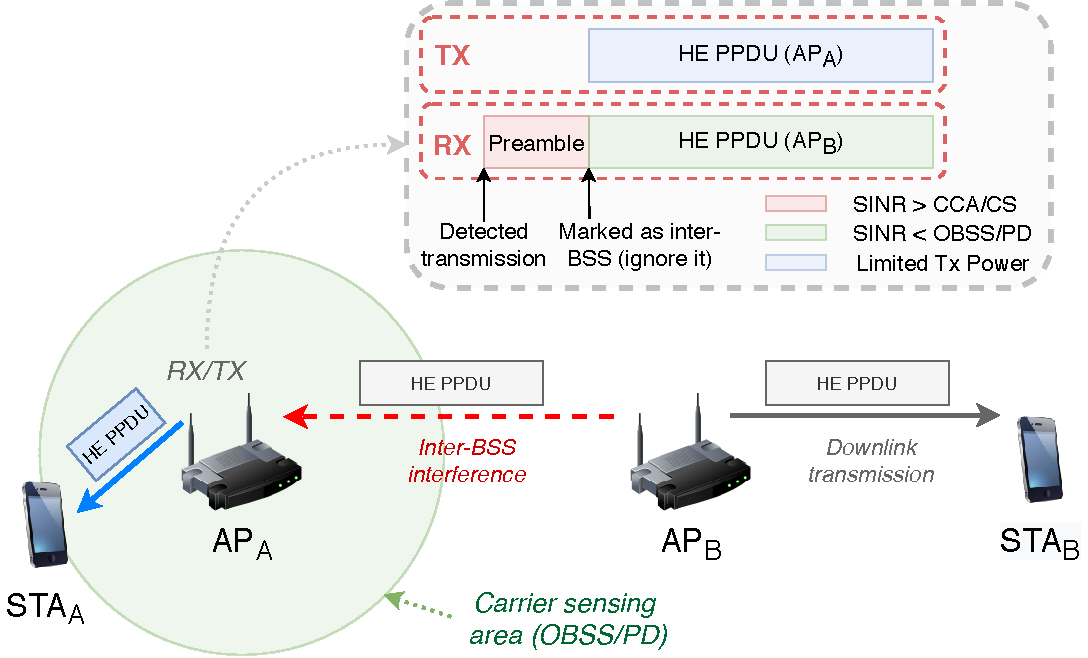
\includegraphics[width=0.8\columnwidth]{images/example_obsspd_sr}
	\caption{Example of OBSS/PD-based SR in a toy scenario.}
	\label{fig:example_obsspd_sr}
\end{figure}

% Analysis of OBSS_PD SR
The performance gains of OBSS/PD-based SR operation have been previously analyzed in \cite{mvulla2018enhanced, qu2018survey, shen2018research,malhotra2019much}. In \textbf{Paper \#5} and \textbf{Paper \#6} we also provide a performance evaluation of 11ax SR. Unlike the previous literature, our performance evaluation is focused on the DL rather than the UL and puts particular emphasis on the analysis of the delay. Moreover, our works target the latest draft (D4.0) of the IEEE 802.11ax amendment.

% PSR 
\subsection{Parametrized Spatial Reuse}
Unlike for OBSS/PD-based SR, PSR aims to exploit Triggered-Based (TB) UL transmissions to carry out SR. Depending on the role of nodes participating in the PSR operation, we find two types of devices: \emph{sharing} (the ones initiating TB transmissions and indicating support for the PSR operation) and \emph{shared} (the ones taking advantage of the PSR opportunities from detected TB transmissions).

For the sake of detecting PSR opportunities, shared devices must check whether their intended transmit power meets the requirements indicated in TB Physical Layer Conformance Procedure (PLCP) Protocol Data Unit (PPDU) from sharing devices. These requirements are based on the maximum level of interference supported by the sharing device. In particular, the intended transmit power cannot exceed the following value:
\begin{equation}
\text{TX\_PWR}_{\max} = \text{TX PWR}_\text{AP} + \text{I}_\text{AP}^{\max} - RPL,
\label{eq:srp_input}
\nonumber
\end{equation}
where $\text{TX PWR}_\text{AP}$ is the normalized transmit power in dBm at the output of the antenna connector, $\text{I}_\text{AP}^{\max}$ is a normalized value in dB that captures the maximum allowed interference at the sharing device,\footnote{$\text{I}_\text{AP}^{\max}$ is computed as the target RSSI indicated in the TF minus the minimum SNR granting a 10\% PER (a safety margin is also included not to exceed 5 dB).} and Received Power Level (RPL) is measured from the legacy portion of the TF (i.e., from PHY headers).

The PSR operation is sketched in Figure \ref{fig:example_psr} for a toy scenario. As shown, the sharing device (i.e., AP$_B$) schedules a UL TB transmission by sending a TF, inspected by the shared device (i.e., AP$_B$) to detect a PSR-based TXOP. 
\begin{figure}[ht!]
	\centering
	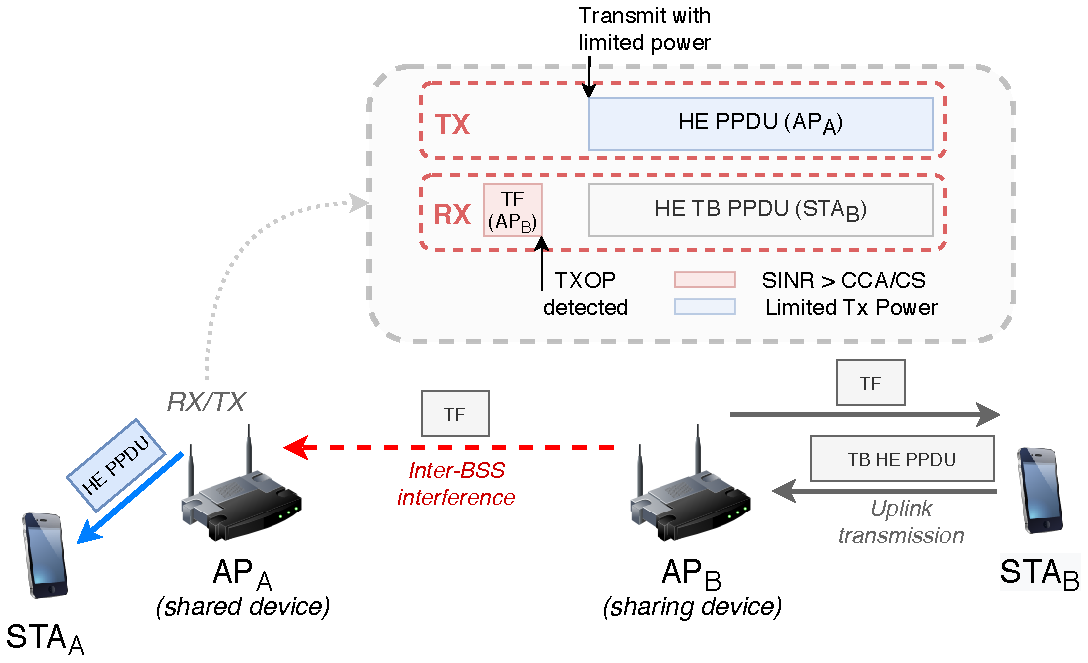
\includegraphics[width=0.8\columnwidth]{images/example_psr}
	\caption{Example of PSR in a toy scenario.}
	\label{fig:example_psr}
\end{figure}

The potential latency gains of PSR have been analyzed in \cite{carvalho2020latency}.  

% 11be and beyond
\section{Spatial Reuse in IEEE 802.11be}
The SR operation included in the 11ax has been shown to provide significant gains for cell-center devices (i.e., devices close to the AP) but lacks applicability in cell-edge users (i.e., devices far from the AP) \cite{qu2019survey}. As a result, the 11be is working on Coordinated SR (CSR) \cite{csr2020}, a cooperative scheme whereby BSSs exchange information (e.g., the acceptable level of interference supported by the different devices) to further enhance the quality of the parallel transmissions achieved through SR. Apart from that, SR is considered to converge with other technologies such as OFDMA \cite{csr2018} and beamforming/null steering \cite{psr2019}. Notice that multi-AP coordination (e.g., coordinated and joint transmission) is one of the main topics that have been so far discussed by IEEE 802.11 task groups \cite{tgbe2018ap}. Besides CSR, the main applications of multi-AP coordination are coordinated beamforming (CBF)  \cite{tgbe2020cbf} and coordinated OFDMA \cite{tgbe2019cofdma}.

Concerning CSR (or Co-SR), it aims to improve the quality of the simultaneous transmissions that can occur due to the SR operation. In particular, the transmit power of secondary transmissions takes into account the maximum level of interference of the target devices whose transmissions are sought to be held. Co-SR is a natural extension of the SR scheme under the multi-AP operation framework and can be implemented with relatively low added complexity. At this stage, the CSR operation is considered to be built upon the following phases:
\begin{itemize}
	 \item \textbf{Preparation:} this phase includes capability announcement (via Beacon or management frames) and monitoring. The AP can request STAs to report the measured RSSI from the neighboring APs and the associated AP so that the Downlink Acceptable Receiver Interference Level (DL ARIL) can be computed. The DL ARIL is used to assess the feasibility of coordinated transmissions and the required transmit power limitations to carry them out.
	%
	\item \textbf{Setup:} the AP winning a TXOP selects the candidate shared AP and indicates the maximum DL ARIL for the following scheduled DL transmission. Then, the shared AP responds to the sharing AP if the channel state is idle.
	%
	\item \textbf{Communication:} the exchange of packets under CSR starts with a trigger frame sent by sharing APs, which choose the set of shared APs to transmit concurrently. The trigger includes information such as the transmission duration, the maximum transmit power allowed or the resource allocation for ACKs. Then, data and ACK packets are exchanged between nodes belonging to the authorized BSSs. The exchange of packets allows the shared APs to update measurements such as the DL ARIL. Finally, the ACK transmission from the STAs received CSR data frame can be performed by UL-OFDMA. However, this approach requires establishing a pre-agreement on the division of the frequency resources.
\end{itemize}

The abovementioned phases are illustrated in Figure \ref{fig:coordinated_sr} for two APs belonging to different BSSs. As it can be noted, the main challenge of CSR lies in data acquisition, which is mainly achieved during the monitoring phase.�This is a critical aspect, especially for highly dynamic deployments. The trade-off between the necessary overhead and the potential gains of coordination hinders CSR's actual performance gains.
\begin{figure}[ht!]
	\centering
	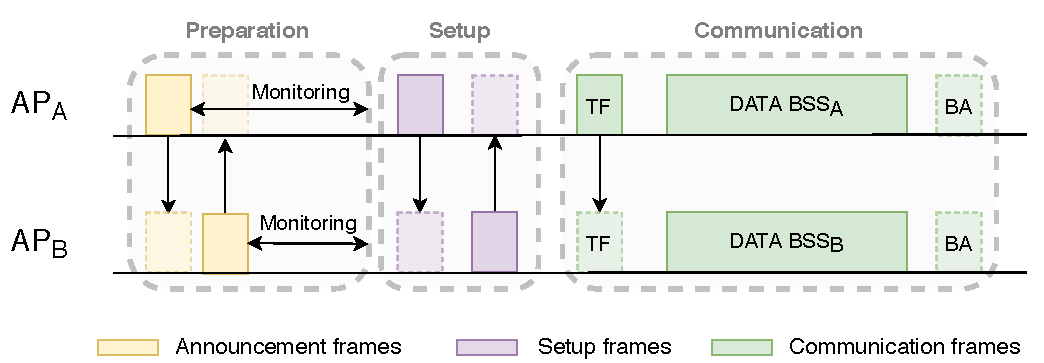
\includegraphics[width=0.8\columnwidth]{images/coordinated_sr}
	\caption{Example of the phases considered for IEEE 802.11be CSR.}
	\label{fig:coordinated_sr}
\end{figure}

%%%%%%%%%%%%%%%%%
% MACHINE LEARNING
%%%%%%%%%%%%%%%%%
\chapter{Machine Learning in WLANs}
\label{chapter3}
ML is meant to empower a computational system for learning, based on experience, so that unseen situations can be properly handled without explicitly being programmed. Concerning wireless communications, the application of ML reveals a big potential because of the following aspects:
\begin{itemize}
	\item First, there is a huge amount of unexploited data generated at both infrastructure and user levels, which could be extremely useful for identifying and exploiting patterns that help at improving network performance.
	\item Second, the increasing complexity of wireless communications problems (e.g., a massive number of concurrent users, ultra low latency applications, very high bandwidth requirements, etc.) complicates the design of hand-crafted solutions. Moreover, complex non-linear phenomena of communications systems (e.g., channel effects, varying traffic requirements, hardware imperfections, etc.) add further complexity. In this regard, ML can learn sophisticated solution strategies from data (model-based vs. data-driven approach), thus granting the ability to adapt to wireless communications problems and characteristics.
	\item Apart from the underlying complex characteristics of problems (e.g., wireless channel), communications systems are built based on functional blocks, each executing well defined and isolated functions (e.g., rate selection, channel allocation, etc.). While individual functions can be separately optimized, their joint operation may further increase end-to-end complexity, thus hindering globally optimized solutions. ML can therefore help to achieve optimal control by addressing the added combinatorial complexity of modularized communications systems.
\end{itemize}

Henceforth, ML is expected to overcome the systemic complexity inherited from novel use cases like Vehicle to Everything (V2X) communications, Machine Type Communications (mMTC), and Ultra-Reliable Low-Latency Communication (uRLLC). In particular, the inherent flexibility of ML for automatically learning diverse situations can address heterogeneous scenarios, including mobility, a massive number of devices, and varying throughput and latency requirements. Because of its high potential for solving complex problems in communications, ML has been applied to a plethora of fields. We address the interested reader to the surveys in \cite{alsheikh2014machine, bkassiny2013survey, wang2016survey, jiang2016machine, zhang2019deep, usama2019unsupervised, klaine2017survey, cayamcela2018artificial, moysen20184g} and references therein.

%In general, the accuracy of a trained ML model is tied to the characteristics of the training data; too diverse and complex patterns may lead to a high level of bias and model overfitting. 

% Architecture
\section{Architectural Aspects for ML-Enabled Communications}

\subsection{Computation Paradigms}

Most popular ML approaches work with batch data, which allows providing powerful solutions and drawing insightful conclusions from typically large datasets. Batch learning methods require certain perennity of data, thus lacking responsiveness and not suiting real-time applications. Notice that large training datasets need significant computational resources to carry out time-consuming tasks. In this regard, online learning mechanisms emerge as a suitable tool to address the non-stationarity of problems whose underlying patterns cannot be fully learned on time. Online learning allows providing fast solutions rather than seeking for optimality (fast and moderate improvement vs. slow optimization). 
The adoption of either batch or online learning mechanisms in telecommunications requires the network infrastructure to accommodate ML-oriented tasks such as data collection, data processing, data analysis, and decision-making \cite{bi2015wireless,chih2017big,wang2018machine}. The procedures mentioned above can be held at different parts of the network, which depends on the network architecture. Batch learning mostly suits to centralized settings where training tasks are held at a single point (e.g., a data center). Centralization allows deriving global ML models encompassing data acquired from multiple sources (e.g., nodes in a network) and even from different domains (e.g., inter-operator data). Furthermore, online learning matches better with decentralized settings, which typically lack powerful equipment but, in turn, allow reducing the complexity of centralized problems by casting them into individual learning problems. Figure \ref{fig:centralized_vs_decentralized} depicts the centralized and decentralized network architectures for ML.

\begin{figure}[ht!]
	\centering
	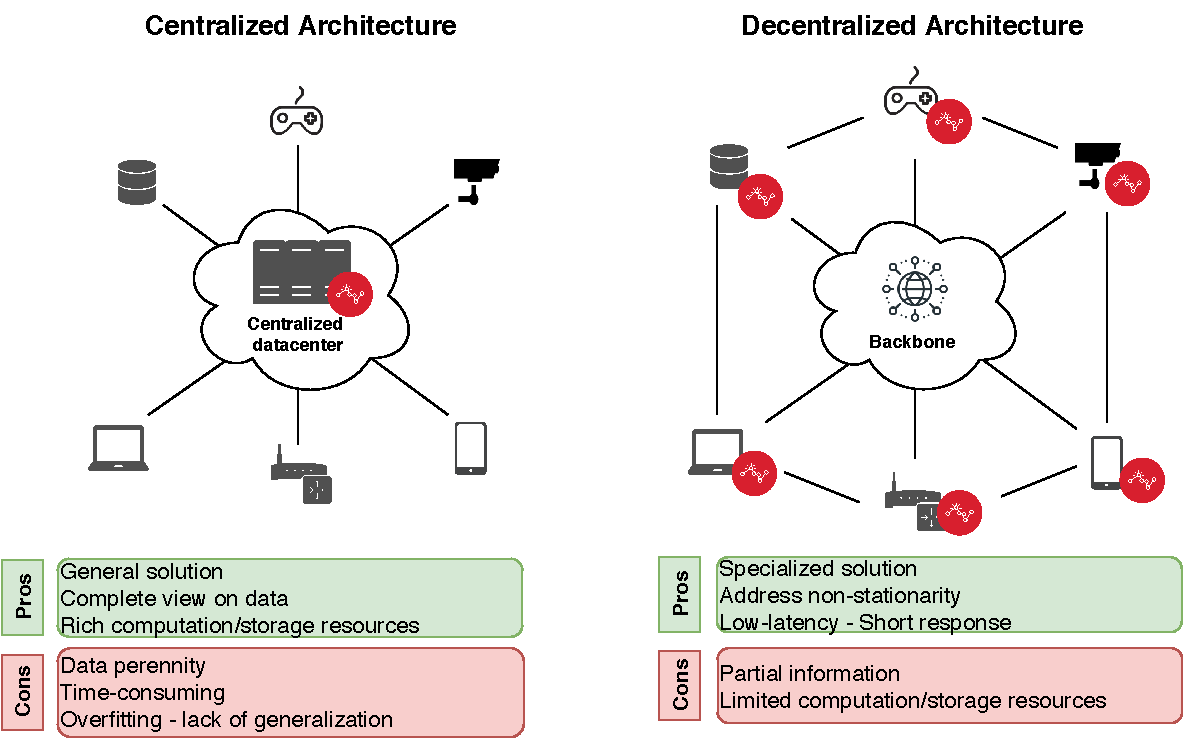
\includegraphics[width=\columnwidth]{images/centralized_vs_decentralized}
	\caption{High-level representation of centralized and decentralized architectures for the application of ML mechanisms in networks.}
	\label{fig:centralized_vs_decentralized}
\end{figure}

In-between centralized and decentralized settings, we find mixed architectures where other learning mechanisms can be applied. For instance, transfer learning (storing knowledge gained while solving one problem and applying it to a different but related problem) \cite{pan2009survey} and federated learning (collaborative training starting from a general model to better fit different contexts and situations) \cite{konevcny2016federated, smith2017federated} can accelerate decentralized approaches by sharing some information among agents (e.g., common solution strategies that can then be personalized for each agent). However, the successful application of these kinds of approaches is tightly tied to the communication capabilities of the implied devices, which defines the degree of cooperation among nodes in a network.

In communications, batch learning has been shown to suit problems related to the core network or involving higher layers of the protocols stack. For instance, Deep Learning (DL) has been broadly applied for predicting periodical patterns of network traffic \cite{zhang2018long, troia2018deep, paul2019traffic} or user mobility \cite{shen2018stepdeep, zhang2020deep, li2019deep}. Alternatively, online learning suits better to problems related to the access network and PHY/MAC layers. In this regard, techniques such as Reinforcement Learning (RL) or sequential learning are widely employed for PHY/MAC optimization. Some examples are resource allocation \cite{xu2017deep}, edge computing \cite{li2018deep, he2018secure}, or MIMO optimization \cite{krishnan2019optimizing}. Notice that time-consuming mechanisms requiring a heavy workload such as Neural Networks (NNs) can be barely applicable to non-stationary problems, which would make trained ML models obsolete very fast.

\subsection{Machine-Learning-Aware Network Architecture}

The first steps towards ML-enabled networking have been recently materialized through the virtualization of networks, i.e., Network Function Virtualization (NFV) and Software-Defined Networks (SDN) paradigms. The fact is that network virtualization provides an unprecedented elasticity for the management and operation of network resources, which were previously limited by traditional hardware-based components. Besides, inter-operator coordination is boosted for bringing the ML operation to a macro-scale level, allowing them to share a vast amount of information and computation resources. These improvements favor the implementation of ML approaches such as federated learning, whereby network infrastructure requires elements to communicate for carrying out a joint decentralized training procedure in an efficient and scalable way.

Currently, the main standardization bodies are progressing on the definition of future ML-aware network architectures. In particular, the following progress has been made:
\begin{itemize}
	\item The 3rd Generation Partnership Project (3GPP) is currently working on the integration of data analytics to network functions \cite{3gpp2019study}.
	\item ETSI groups on Experiential Networked Intelligence (ENI) and Zero-touch network and Service Management (ZSM) are actively studying the integration of AI to networks \cite{etsi2019architecture}.
	\item ITU-T has released a set of specifications on a \emph{Unified architecture for 5G and beyond} \cite{itu2019architecture, itu2019data}. Remarkably, ITU's standardized architecture provides a common nomenclature for ML-related mechanisms so that interoperability with other networking systems is achieved. 
\end{itemize} 

In \textbf{Paper \#7}, we proposed a realization of the ITU-T ML-aware architecture for IEEE 802.11 WLANs. Through the definition of ML components and management functions, the ITU-T architecture provides the necessary flexibility for fulfilling different use case requirements, ranging from centralized solutions to local-learning approaches. This is particularly suitable for Wi-Fi deployments, which may lack powerful centralized equipment for gathering data and processing it (e.g., residential scenarios). In these cases, it is imperative to flexibly instantiate ML pipeline nodes, thus adapting to the set of available resources and capabilities from each use case.

The ITU-T ML-aware architecture defines a set of components and procedures to enable the usage of ML models in networking operations. In particular, the following main components are defined:
\begin{itemize}
	\item \textbf{ML pipeline:} set of logical nodes that are combined to form an ML application in a network. ML pipeline nodes are responsible for data collection, data processing, ML model application, and output distribution.
	\item \textbf{ML management and orchestration:} logical node to manage and orchestrate ML pipelines according to use case specifications.
	\item \textbf{ML sandbox:} isolated domain for training, testing, and evaluating ML pipeline nodes before being deployed in a production environment.
 	\item \textbf{Data handling blocks:} framework to handle ML data collection, ML data processing, and ML data output.
\end{itemize}

Figure \ref{fig:itu_architecutre} shows the high-level architectural components defined in \cite{itu2019architecture}. As illustrated, the modularized ML operation may take place at any point in the network. As a result, the chaining and deployment of ML pipeline nodes are flexible and depend on the use case.
 
\begin{figure}[ht!]
	\centering
	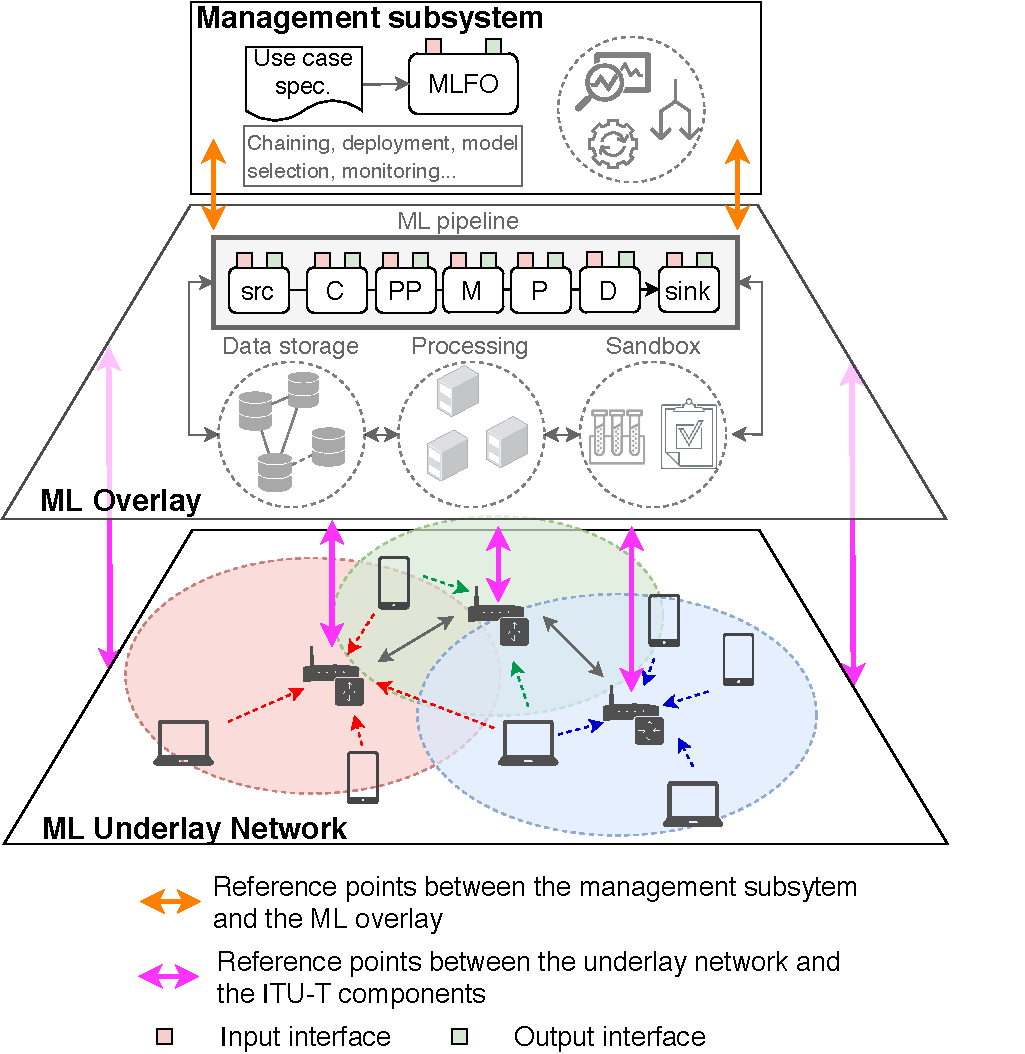
\includegraphics[width=.8\columnwidth]{images/itu_architecutre}
	\caption{ITU-T's high-level architecture for future ML-aware networks.}
	\label{fig:itu_architecutre}
\end{figure}

Among the architectural components of the ITU-T architecture, we paid particular attention to the ML sandbox. In this regard, \textbf{Paper \#8} delves into the potential usage of network simulators to enhance the reliability of ML for communications. In particular, we showcased that network simulators can be used to validate the performance of ML methods before applying them to live networking systems. To that purpose, we provided a proof-of-concept testbed implementation of a residential WLAN deployment, which was empowered with an ML model trained in a network simulator. Besides validation purposes, simulators are useful for generating synthetic data sets that can be used for training (e.g., predicting unforeseen situations from which there are no real data).

% MABs
\section{Multi-Armed Bandits in Communications}
The \emph{learning by experience} characteristic of sequential learning suits WLANs well because it allows addressing complex partial information problems. The fact is that WLANs pose a set of specific challenges resulting from their multiple deployment modes (e.g., campus network, residential usage) and their typical decentralized nature. Although WLANs can count with plenty of data to be used by ML methods in large and planned deployments, we find other types of scenarios (e.g., residential deployments) were data may fail to be integrated at a single point due to potential computation, storage, or communication limitations (e.g., end devices may have low-throughput connections and be intermittently available). Besides, the varying nature of WLAN deployments (e.g., due to STAs mobility) leads to a high non-stationarity.

%\subsection{The MAB Framework}
In the MAB problem, \cite{thompson1933likelihood, bush1953stochastic}, and as for classical RL formulations, an agent (or learner) interacts with the environment to accumulate knowledge that allows adapting to underlying changes in the reward distribution over time. The maximization of a long-term goal \cite{auer2002finite} requires finding an equilibrium between exploration (improve your knowledge) and exploitation (obtain the maximum profit based on your experience).

% MABs formulation
Formally, a learner sequentially picks actions $a_t \in K$ and observes their reward vector $r_t$ over a time horizon $T$. Typically, the reward is granted by what is known as the environment, which may be of diverse nature (e.g., stochastic distribution, adversarial payoff). In the bandits setting, rewards are generated by hidden distributions, and their value is only revealed once the corresponding arm is played. Bandits differ from \emph{partial} and \emph{full} information settings that reveal the reward of a set or all the possible actions, respectively. 

The performance of a given action-selection strategy is typically measured by the regret $R_T$, which compares the performance achieved by the selected actions with the best fixed action in hindsight. In general, an algorithm is said to learn if its regret grows sublinearly. Typical good performance is achieved for $R_T \in \mathcal{O}(\sqrt{T})$ or even $R_T \in \mathcal{O}(\log{}T)$. 

% Types of MABs and contexts of application
Despite its simplicity, the bandits framework stands as a compelling solution for decision-making problems. The main reason is that bandit feedback (i.e., the agent only gets information of actions as it plays them) is easier to be provided in practice than full or partial feedback (i.e., information of other actions are provided even if not being played). The most typical bandits applications are web advertising, sales optimization, online recommendations, resource allocation, and packet routing, among many others. A plethora of bandits formulations exist according to multiple assumptions that extend the basic bandits game. The different MAB formulations are based on multiple aspects: the statistics behind rewards (e.g., stochastic vs. non-stochastic bandits), the availability of actions (e.g., sleeping bandits, mortal bandits), the type of Markovian settings (e.g., rested vs. restless bandits), the nature of the environment (e.g., adversarial bandits), and a very long etcetera of variations. The bandits problem has been treated in detail by several books and surveys. Table \ref{tab:bandits_categories} provides a high-level categorization of the most popular types of bandits. We encourage the interested reader to delve into the works in \cite{cesa2006prediction, gittins2011multi, bubeck2012regret, lattimore2018bandit, slivkins2019introduction}.

\begin{table}[ht!]
	\centering
	\caption{High-level categorizations of most popular bandits types.}
	\label{tab:bandits_categories}
	\begin{tabular}{|l|l|}
		\hline
		\multicolumn{1}{|c|}{\textbf{Categorization Criteria}} & \multicolumn{1}{c|}{\textbf{Bandits models}} \\ \hline
		Reward generation process & \begin{tabular}[c]{@{}l@{}}Stochastic, adversarial, Markovian \\ (rested/restless)\end{tabular} \\ \hline
		Reward function & \begin{tabular}[c]{@{}l@{}}Discrete, continuum (linear/nonlinear), \\ Lipschitz, Gaussian\end{tabular} \\ \hline
		Feedback type & \begin{tabular}[c]{@{}l@{}}Full information, bandit, \\ semi-bandit, partial monitoring\end{tabular} \\ \hline
		State-awareness & Contextual bandit \\ \hline
	\end{tabular}
\end{table}

%\subsection{MAB in Communications}
In wireless communications, many problems have statistical characteristics that can be approximated with mathematical models. In this regard, MAB-based applications have shown great potential for optimizing a plethora of problems. Some examples are channel selection \cite{gai2010learning}, spectrum access \cite{tekin2011online}, transmission scheduling \cite{chen2006transmission}, or AP selection \cite{carrascosa2019decentralized}. Table \ref{tab:mabs_communications} provides an overview of some popular MAB-based applications in communications.

\begin{table}[]
	\caption{Overview of bandit-based applications for communications}
	\label{tab:mabs_communications}
	\resizebox{\textwidth}{!}{%
		\begin{tabular}{|l|l|l|l|l|}
			\hline
			\multicolumn{1}{|c|}{\textbf{Problem}} & \multicolumn{1}{c|}{\textbf{Modeling}} & \multicolumn{1}{c|}{\textbf{Goals}} & \multicolumn{1}{c|}{\textbf{\begin{tabular}[c]{@{}c@{}}Baseline \\ algorithms\end{tabular}}} & \multicolumn{1}{c|}{\textbf{References}} \\ \hline
			\begin{tabular}[c]{@{}l@{}}Opportunistic \\ spectrum access \& \\ Channel selection\end{tabular} & \begin{tabular}[c]{@{}l@{}}Stochastic, non-stochastic, \\ restless, contextual, Markovian\\ bandits\end{tabular} & \begin{tabular}[c]{@{}l@{}}Decentralized optimal allocation, \\ optimize number of secondary\\ transmissions, $\epsilon$-correct ranking\end{tabular} & \begin{tabular}[c]{@{}l@{}}UCB, $\epsilon$-greedy,\\ calibrated forecasting\end{tabular} & \cite{liu2008restless,gai2010learning, tekin2011online,anandkumar2011distributed,rosenski2016multi,maghsudi2015channel} \\ \hline
			Power control & Non-stochastic bandits & Optimize SINR & \begin{tabular}[c]{@{}l@{}}Follow the perturbed leader,\\ exponential weighted average\end{tabular} & \cite{maghsudi2014joint} \\ \hline
			User association & \begin{tabular}[c]{@{}l@{}}Sleeping, Bernoulli,\\ non-stochastic bandits\end{tabular} & Energy saving, improve the throughput & UCB, $\epsilon$-greedy & \cite{maghsudi2017distributed,carrascosa2020multi} \\ \hline
			Inter-cell coordination & \begin{tabular}[c]{@{}l@{}}Adversarial, stochastic,\\ non-stochastic,\\ contextual bandits\end{tabular} & \begin{tabular}[c]{@{}l@{}}Optimize inter-cell frequency resources,\\ energy saving, map SON configurations \\ and operator objectives\end{tabular} & EXP3, UCB, $\epsilon$-greedy & \cite{coucheney2015multi, feki2011autonomous, ayala2018contextual, daher2017cognitive} \\ \hline
			Dynamic rate selection & Structured, Markovian bandits & \begin{tabular}[c]{@{}l@{}}Maximize the number of packets \\ successfully transmitted, \\ learn changes in the channel\end{tabular} & UCB & \cite{combes2014dynamic, zhao2020non} \\ \hline
			LTE/Wi-Fi coexistence & Convex bandits & Fair channel sharing & Online gradient descent & \cite{cano2018wireless} \\ \hline
		\end{tabular}%
	}
\end{table}

% Nexus with Game Theory and why equilibrium can be reached
Concerning decentralized SR in wireless networks, it can be naturally defined as a multi-agent (or multi-player) problem. Each individual (e.g., a BSS) has player-specific goals and rewards. The maximum achievable performance of a node depends on its transmission capabilities, the interference it senses, the traffic load it needs to serve and/or receive, etc. The multi-agent approach allows capturing the distributed nature of IEEE 802.11 WLANs and keeping dimensionality low for the SR problem. However, it may lead to a competition among players, thus revealing a nexus with game theory. A player attempts to maximize a long-term reward in a single-agent system by interacting with an environment (which can be stochastic or non-stochastic) in isolation. Under this setting, performance guarantees can be straightforwardly provided, even if dealing with adversarial \cite{auer2002nonstochastic} or dynamic environments \cite{gupta2011thompson}. In contrast, weaker performance guarantees can be provided for multi-agent systems. Notice that, in the multi-player setting, the reward of an agent depends on what all (or some) of the other agents do, which leads to non-stationarity. As a result, the knowledge acquired by agents becomes quickly outdated.

Most of the current literature in multi-player MABs for wireless communications is based on the channel access problem in cognitive radio \cite{gai2010learning, liu2008restless, anandkumar2011distributed, di2011learning, bkassiny2013survey, cohen2014restless, abbas2015recent, maghsudi2015joint, avner2014concurrent}. The cognitive radio characteristics make it a suitable and attractive problem to be modeled with the bandits framework. In particular, each node attempts to access the channel represents a player, and channels are arms (or bandits). In general, rewards are granted to players in a binary fashion, ``1'' if the channel can successfully be accessed, or ``0" otherwise (two or more nodes select the same channel). Accordingly, each player has the same view on actions (different players playing the same action obtain the same payoff), which makes the game smooth, i.e., the player's reward function is continuous concerning the entire strategy set. Table \ref{tab:mpmab_cr} analyzes the state-of-the-art approaches taken for modeling channel access in cognitive radio through multi-player MABs, which make use of popular baseline algorithms such as $\varepsilon$-greedy \cite{auer2002finite}, upper confidence bound (UCB) \cite{lai1985asymptotically, agrawal1995sample}, exponential weight algorithm for exploration and exploitation (EXP3) \cite{auer1995gambling, auer2002finite}, and Thompson sampling \cite{thompson1933likelihood}.

\begin{table}[]
	\caption{State-of-the-art multi-player MAB solutions for channel access in cognitive radio.}
	\label{tab:mpmab_cr}
	\resizebox{\textwidth}{!}{%
		\begin{tabular}{|c|l|l|l|}
			\hline
			\textbf{Work} & \multicolumn{1}{c|}{\textbf{Approach}} & \multicolumn{1}{c|}{\textbf{Requirements}} & \multicolumn{1}{c|}{\textbf{Results}} \\ \hline
			\cite{anandkumar2011distributed} & \begin{tabular}[c]{@{}l@{}}Distributed mechanism that \\ combines sensing with randomized \\ access to learn channel statistics \\ and the activity of other users\end{tabular} & \begin{tabular}[c]{@{}l@{}}- The number of users is fixed and known\\ - Channel sensing is perfect\\ - All the players use the same strategy\\ - Binary reward (free/collision)\end{tabular} & \begin{tabular}[c]{@{}l@{}}Order-optimal regret with \\ logarithmic lower bound\end{tabular} \\ \hline
			\cite{liu2010distributed} & \begin{tabular}[c]{@{}l@{}}Decentralized time-division fair \\ sharing of the best arms\end{tabular} & \begin{tabular}[c]{@{}l@{}}- i.i.d. reward\\ - Conditions of linearity, continuity, \\ and density for unknown parameters\\ - Binary reward (free/collision)\\ - The number of users is fixed and known\end{tabular} & \begin{tabular}[c]{@{}l@{}}Same logarithmic regret order \\ as for collaborative approach \\ where nodes exchange observations \\ and make decisions jointly\end{tabular} \\ \hline
			\cite{di2011learning} & \begin{tabular}[c]{@{}l@{}}Collaborative mechanism based on\\ slotted periods (decision, sensing,\\ transmission, communication)\end{tabular} & \begin{tabular}[c]{@{}l@{}}- Channel sensing is done\\ - CSMA/CA is used by secondary users\\ - Rewards are broadcasted\\ - Same channel conditions for all users\end{tabular} & \begin{tabular}[c]{@{}l@{}}Linear regret improving random\\ and greedy channel access schemes\end{tabular} \\ \hline
			\cite{maghsudi2015channel} & \begin{tabular}[c]{@{}l@{}}Distributed no-regret learning with\\ calibrated forecaster\end{tabular} & \begin{tabular}[c]{@{}l@{}}- The joint action profile is known\\ - All the players use the same strategy\\ - Time-invariant average channel gains\end{tabular} & \begin{tabular}[c]{@{}l@{}}Global optimal solution and \\ convergence to correlated equilibria\end{tabular} \\ \hline
			\cite{avner2014concurrent} & \begin{tabular}[c]{@{}l@{}}Non-cooperative selfish approach\\ based on $\epsilon$-greedy exploration \\ and CSMA/CA\end{tabular} & \begin{tabular}[c]{@{}l@{}}- K $\geq$ N ($K$: channels, $N$: users)\\ - The number of users is fixed and known\end{tabular} & \begin{tabular}[c]{@{}l@{}}Sub-linear regret and convergence to \\ system-optimal solution\end{tabular} \\ \hline
			\cite{gai2010learning} & \begin{tabular}[c]{@{}l@{}}Centralized method for combinatorial\\ bandits with user-channel pairs\end{tabular} & \begin{tabular}[c]{@{}l@{}}- K $\geq$ N ($K$: channels, $N$: users)\\ - Throughput as an i.i.d. random variable\\ - Coordination/synchronization\end{tabular} & \begin{tabular}[c]{@{}l@{}}Upper bound regret that grows \\ polynomially with the combinatorial \\ number of users and channels\end{tabular} \\ \hline
		\end{tabular}%
	}
\end{table}

\section{Multi-Armed Bandits for Decentralized Spatial Reuse: Between ML and Game Theory}

In \textbf{Paper \#1}, \textbf{Paper \#2}, and \textbf{Paper \#3}, we have addressed decentralized SR through multi-player MABs, which allowed us to reduce the combinatorial complexity of the problem.\footnote{Notice that the number of configurations in an OBSS grows exponentially with the number of BSS to be optimized.} In particular, each agent (or player) $p\in \mathcal{P}$ represents a BSS in an OBSS. The actions $a\in \mathcal{A}_p$ that each agent can choose are defined as combinations of sensitivity and transmit power values, which lead to agent-specific rewards $r \in \mathcal{R}_p$. Notice that individual rewards depend on the joint action profile, i.e., the global configuration in BSSs, due to the spatial interactions between nodes. Algorithm \ref{alg:sr_mabs} describes the decentralized SR game in general terms. The procedure mentioned above is enabled by a monitoring phase (time between iterations), whereby agents collect information of the performance granted by the actions being selected, which depend on the joint action profile (see Figure \ref{fig:paper_5_learning_procedure}).

\begin{algorithm}[h!]
	\SetKwInOut{Input}{Input}
	\SetKwInOut{Output}{Output}		
	Function MAB $(\mathcal{A})$\;
	\Input{$\mathcal{A}_p$: set of possible actions in \{$1, ..., K$\} to be selected by each player $p\in \mathcal{P}$}
	initialize: $t=0$,  for each arm $k \in \mathcal{A}_p$, set $r_{p,k} = 0$ and $n_{p,k} = 0$ \\
	\While{active}
	{
		\For{each $p\in \mathcal{P}$}  {
		Play arm $k \in \mathcal{A}_p = \underset{i=1,...,K}{\text{argmax }} \theta_i $ \\
		Observe the reward obtained $r_{p,k}(t)$\\			
		Compute the reward $r_{k,t}$ \\
		$n_{k,t} \leftarrow n_{k,t} + 1$\\
		}
		Update the estimation function $ \theta $\\
		$t \leftarrow t + 1$
	}	
	\caption{Decentralized SR game through MABs}
	\label{alg:sr_mabs}
\end{algorithm}	

\begin{figure}[ht!]
	\centering
	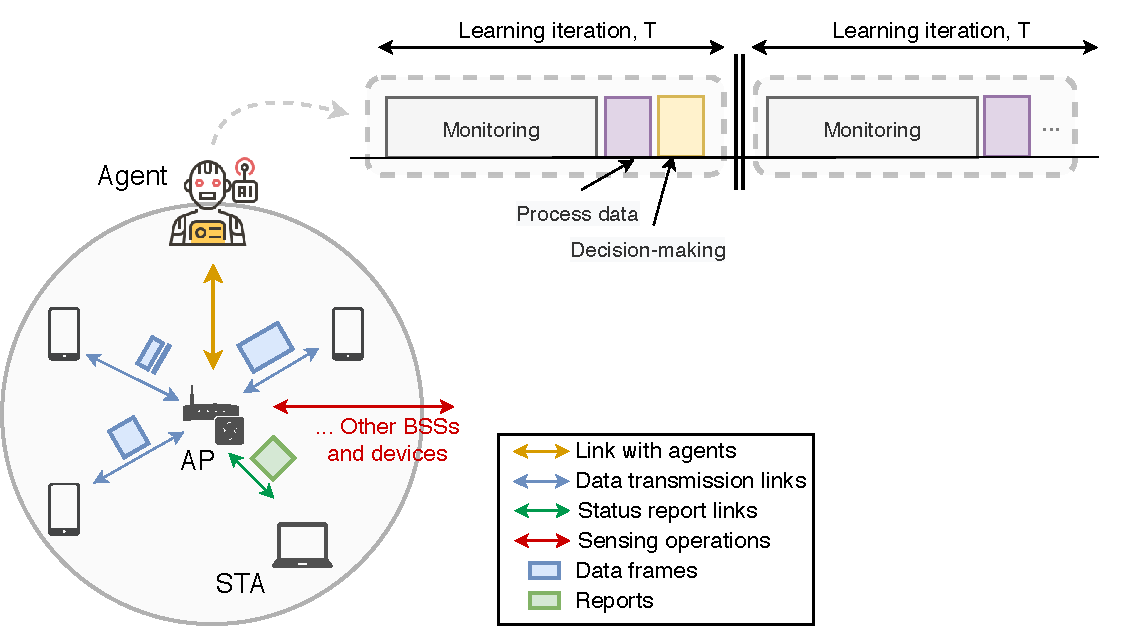
\includegraphics[width=0.8\textwidth]{images/paper_5_learning_procedure}
	\caption{Sequential learning procedure carried out in IEEE 802.11 WLANs.}
	\label{fig:paper_5_learning_procedure}
\end{figure}

In \textbf{Paper \#1} and \textbf{Paper \#2}, we have proposed a selfish method whereby agents learn towards maximizing local reward. Specifically, several concurrent agents attempt to improve their performance, based on local information. The effectiveness of this method is tightly coupled to the global reward. In potential games \cite{monderer1996potential}, a class of problems for which individual agents are connected to a global function with a unique maximum, optimizing local rewards also brings the whole system closer to the unique global optimum. For instance, the work in \cite{maghsudi2015joint} addresses transmission power control and channel access in a distributed manner. According to a simplified model of opportunistic spectrum access, the authors can provide distributed no-regret strategies that lead to the set of correlated equilibria. However, some assumptions are made to define a unique maximum in the global performance function so that convergence guarantees to the optimum can be provided. In particular, the reward function used by the players is continuous with respect to the strategy set, which is also bounded. Intuitively, this means that the social cost that any action incurs to the other players can be linearly quantified.

Therefore, in multi-player MABs, optimal solutions can typically be provided only to tractable problems that are generally linear, stationary, and generated by independent stochastic processes (e.g., with underlying Gaussian statistics). This is not the case of the proposed decentralized SR solution, in which it is not possible to provide a distributed no-regret strategy that converges to an optimal equilibrium. The fact is that the joint reward function of the SR problem with multiple concurrent players does not have a unique optimum. The set of correlated equilibria cannot be then characterized. In particular, the following properties differing from distributed channel access prevent to do so:
\begin{enumerate}
	\item Spatial interactions inflict abrupt changes to the reward obtained by a BSS, which can be based, for instance, on the throughput. To put an example, increasing the sensitivity contributes to reducing contention, but it may lead to noticing a higher amount of interference during transmissions. 
	\item Besides, considering the worst-case interference (devices transmitting continuously) is an unrealistic assumption. Therefore, the social-cost of actions varies with time and according to the transmissions done on a per-packet-basis (where certain randomness is added due to many causes such as channel effects, retransmissions, the randomized backoff procedure, etc.).
\end{enumerate}

In these situations, defining a shared learning goal in multi-agent systems is not trivial because rewards are not equally assigned to agents. Each reward depends on the joint action profile. Nonetheless, the MABs framework remains a powerful solution to address real-world problems with complex and unpredictable phenomena behind reward distributions. The multi-player setting (i.e., multiple agents attempt to learn concurrently) allows for tackling smaller individual problems rather than attempting to solve the full centralized problem. While this leads to non-stationary, on-time improvements prevail over long-term optimality.

As an alternative to the selfish approach, a collaborative setting was also proposed in \textbf{Paper \#3}, whereby agents attempt to maximize a shared reward. In particular, we defined the max-min throughput to be improved by a set of overlapping BSSs. Note, as well, that the learning procedure is kept decentralized (each agent is responsible for selecting its actions). The collaborative approach is meant to boost fairness, but as for the selfish setting, its effectiveness towards optimality is limited by the shape of the global performance function. 

%%%%%%%%%%%%%%%%%
% METHODS
%%%%%%%%%%%%%%%%%
\chapter{Methodology and Enablers} 
\label{chapter4}
The use of analytical models and simulation tools is crucial for studying and understanding novel technologies such as SR. In this Chapter, we present the analytical and simulation tools that have been used for that purpose. In particular, we developed an analytical model to address the complex inter-BSS interactions posed by the SR operation. Besides, given the lack of simulation tools to characterize such a new technology, we developed an IEEE 802.11ax-based network simulator. The purpose of this simulator is twofold. First, we need it to evaluate the performance of SR in dense deployments at a macro-scale level, so that we can provide a first taste of the potential advantages and implications of SR. Notice that current well-known simulation tools like ns-3 can be complex to extend due to the high level of detail put in both MAC and PHY layers. Besides, simulating highly dense deployments can be costly or even intractable in terms of time and computational resources. Second, due to the primary purpose of this thesis on studying the application of ML models for SR, the simulator was developed for supporting the operation of intelligent agents. 

% CTMNs model
\section{Spatial Reuse through Continuous Time Markov Networks}

The Bianchi model \cite{bianchi2000performance} has been widely adopted by the research community as a reference for analyzing the throughput of IEEE 802.11 WLANs. However, this model only focuses on the MAC layer and requires all the analyzed nodes to be in the same coverage area. To model SR, it is important to capture the dynamic PHY interactions when tuning the sensitivity threshold and the transmit power.

The analysis of SR has been previously addressed in multiple ways. Most of the models are based on signal-to-interference-plus-noise ratio (SINR) \cite{gupta2000capacity} and include the concept of physical carrier sensing to capture inter-device interactions. We find a plethora of works that build upon SINR-based models for meeting several purposes (model RTS/CTS, etc.) \cite{guo2003spatial, hekmat2004interference,yang2005physical, yang2007modeling}. Typically, SINR-based models use the concepts described in Table \ref{tab:conditions_sr}. First, the device's sensitivity allows defining the transmission range of a given transmitter-receiver pair based on fixed transmit power. Second, the carrier sensing threshold determines the idle/busy channel condition from a transmitter node's point of view. The carrier sensing threshold has been widely used for defining the carrier sense area (alternatively, the set of carrier sense nodes) or the silence set (i.e., the set of nodes that detect the channel busy if a given node transmits). Finally, the capture effect includes interfering nodes' operation, thus allowing to define the interference range (alternatively, the set of interfering devices). While SINR-based methods are useful to derive interactions among devices in the spatial dimension, they consider the worst-case interference (i.e., nodes are assumed to transmit permanently). This assumption entails neglecting spectrum access coordination and hence losing insights on the MAC operation.

\begin{table}[]
	\centering
	\caption{Concepts to model spatial reuse in wireless networks.}
	\label{tab:conditions_sr}
	\resizebox{\textwidth}{!}{%
		\begin{tabular}{|l|l|l|}
			\hline
			\multicolumn{1}{|c|}{\textbf{Concept}} & \multicolumn{1}{c|}{\textbf{Description}} & \multicolumn{1}{c|}{\textbf{Function}} \\ \hline
			Sensitivity & \begin{tabular}[c]{@{}l@{}}A receiver can detect a transmission if its \\ received power is greater than the sensitivity \\threshold\end{tabular} & -  Determine the transmission range \\ \hline
			Carrier sensing & \begin{tabular}[c]{@{}l@{}}A node cannot initiate a transmission if the \\ power it senses is above its carrier sense\\ threshold\end{tabular} & \begin{tabular}[c]{@{}l@{}}- Determine the carrier sense set\\ - Determine the carrier sense range\\ - Determine the silence set\end{tabular} \\ \hline
			Capture effect & \begin{tabular}[c]{@{}l@{}}A receiver can decode a signal if the SINR \\ is above a given threshold\end{tabular} & \begin{tabular}[c]{@{}l@{}}- Define the interference range\\ - Determine the interference set\end{tabular} \\ \hline
		\end{tabular}%
	}
\end{table}

Another field that is attracting a lot of attention is stochastic geometry (SG), which allows modeling the random nature of dense wireless networks. In particular, SG allows deriving statistical properties of the underlying interactions among a random set of nodes (typically, set according to random point processes). In telecommunications, SG has been widely applied to model the behavior of users and to estimate metrics such as the outage probability or the throughput per area \cite{elsawy2016modeling}. Concerning SR, we highlight the works in \cite{zhao2016stochastic, zhang2015stochastic, zhong2016stochastic, iwata2019stochastic}, which provided models based on SG to capture the effect of tuning the sensitivity threshold in WLANs. However, SG models mainly focus on PHY layer effects and fail to capture the asymmetries that may occur when applying the SR operation, which also involves the tuning of the transmit power.

In \textbf{Paper \#5}, we introduced Continuous Time Markov Networks (CTMNs) \cite{bellalta2014throughput,bellalta2017throughput} to analytically model the SR operation, thus capturing both MAC and PHY layers interactions. This model allowed us to provide insights into the inter-BSS interactions resulting from SR, which has been key to develop the mechanisms proposed in this thesis. %\cite{jiang2018stochastic}: hybrid SG and CTMC.

The CTMN model captures the CSMA/CA operation used in IEEE 802.11 WLANs through states representing the set of BSSs that are transmitting at a given moment. Transitions between states occur when BSSs start a transmission (i.e., they gain access to the medium) or when the transmission finishes (i.e., they abandon the channel). It is important to highlight that the CTMN model considers additive interference, which results from the combination of different simultaneous interfering transmissions. Accordingly, we are able to characterize real deployments where spatially-distributed interactions occur. Concerning this model, the following assumptions are considered:
\begin{enumerate}
	\item The backoff procedure for accessing the medium is continuous in time, which is useful for modeling the attempt rate of transmitters as a Poisson process. However, this assumption prevents modeling collisions due to backoff expiring at the same instant.
	\item Data transmissions are downlink only, which relaxes the complexity of the problem and allows us to focus only on inter-AP interactions. Notice that a state in the Markov chain represents a set of nodes transmitting in an OBSS. As a result, the complexity of the model grows in a combinatorial manner.  
	\item To be consistent with the previous assumption, uplink transmissions of control packets (e.g., ACKs) are only considered for computing the total transmission time. This leads not to consider uplink transmissions for modeling inter-BSS interactions.
	\item Full-buffer traffic is considered for the sake of analyzing the interactions resulting from SR more lucidly.
\end{enumerate}

The CTMN model is very useful to understand the new kind of inter-AP interactions resulting from the 11ax SR operation. Besides, it allows us to validate the implementation of SR done at the simulator, which is later introduced in Section \ref{section_4_2}. A disadvantage of the CTMN model is its lack of scalability for characterizing crowded deployments. Modeling dense scenarios becomes intractable since the number of feasible states increases in a combinatorial manner with the number of BSSs.

% 11ax OBSS/PD-based SR
\subsection{IEEE 802.11ax OBSS/PD-based Spatial Reuse}

To model the 11ax SR operation, we consider new states for capturing the different situations created by the sensitivity levels and the corresponding transmit power limitation to be employed by each BSS in a given scenario. First, tuning the OBSS/PD of a BSS allows finding new types of inter-BSS interactions that could not exist without applying SR (i.e., a new set of states modeling concurrent transmissions). Moreover, the transmit power limitation in new states has implications on the capabilities of BSSs. Notice that a lower transmission power entails a more robust Modulation and Coding Scheme (MCS) and, as a consequence, a lower data rate.

Figure \ref{fig:model_11ax_sr} illustrates the application of the proposed CTMN model for a simple deployment. In particular, we consider two BSSs that can transmit concurrently, provided that one of them (namely, BSS$_A$) applies OBSS/PD-based SR. Figure \ref{fig:ctmn_sr_1} shows the considered deployment, where the carrier sense area of AP$_A$ is illustrated for two different carrier sensing approaches. First, the default CCA/CS threshold (shown in red) makes AP$_A$ sense the channel busy when AP$_B$ is transmitting, thus preventing parallel transmissions to occur. In contrast, the OBSS/PD threshold (shown in green) allows AP$_A$ ignoring AP$_B$'s transmissions and therefore access the channel. Note, as well, that the lower OBSS/PD threshold entails reducing the transmit power, which leads to a lower MCS index. These interactions are captured by the corresponding CTMN (see Figure \ref{fig:ctmn_sr_2}). As shown, BSS$_A$ can transmit in two different manners (noted by $A$ and $A_{SR}$, respectively), which extend legacy interactions with SR channel access rules and corresponding nodes' capabilities. Notice that the transmit power limitation when applying the OBSS/PD threshold makes BSS$_A$ to use a more robust MCS, thus sacrificing capacity. In exchange, it is possible to hold simultaneous transmissions when BSS$_B$ occupies the channel.

\begin{figure}[ht!]
	\centering
	\subfigure[Deployment]{\label{fig:ctmn_sr_1}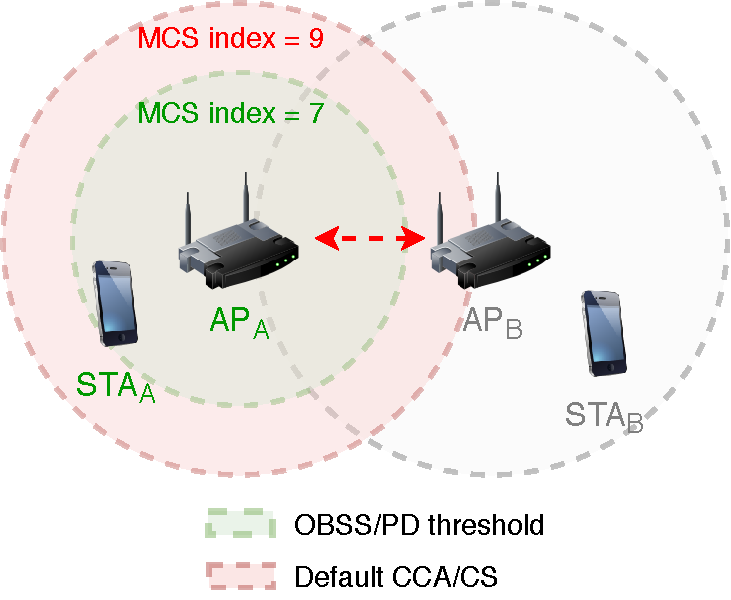
\includegraphics[width=0.4\textwidth]{images/ctmn_sr_1}}
	\subfigure[CTMN]{\label{fig:ctmn_sr_2}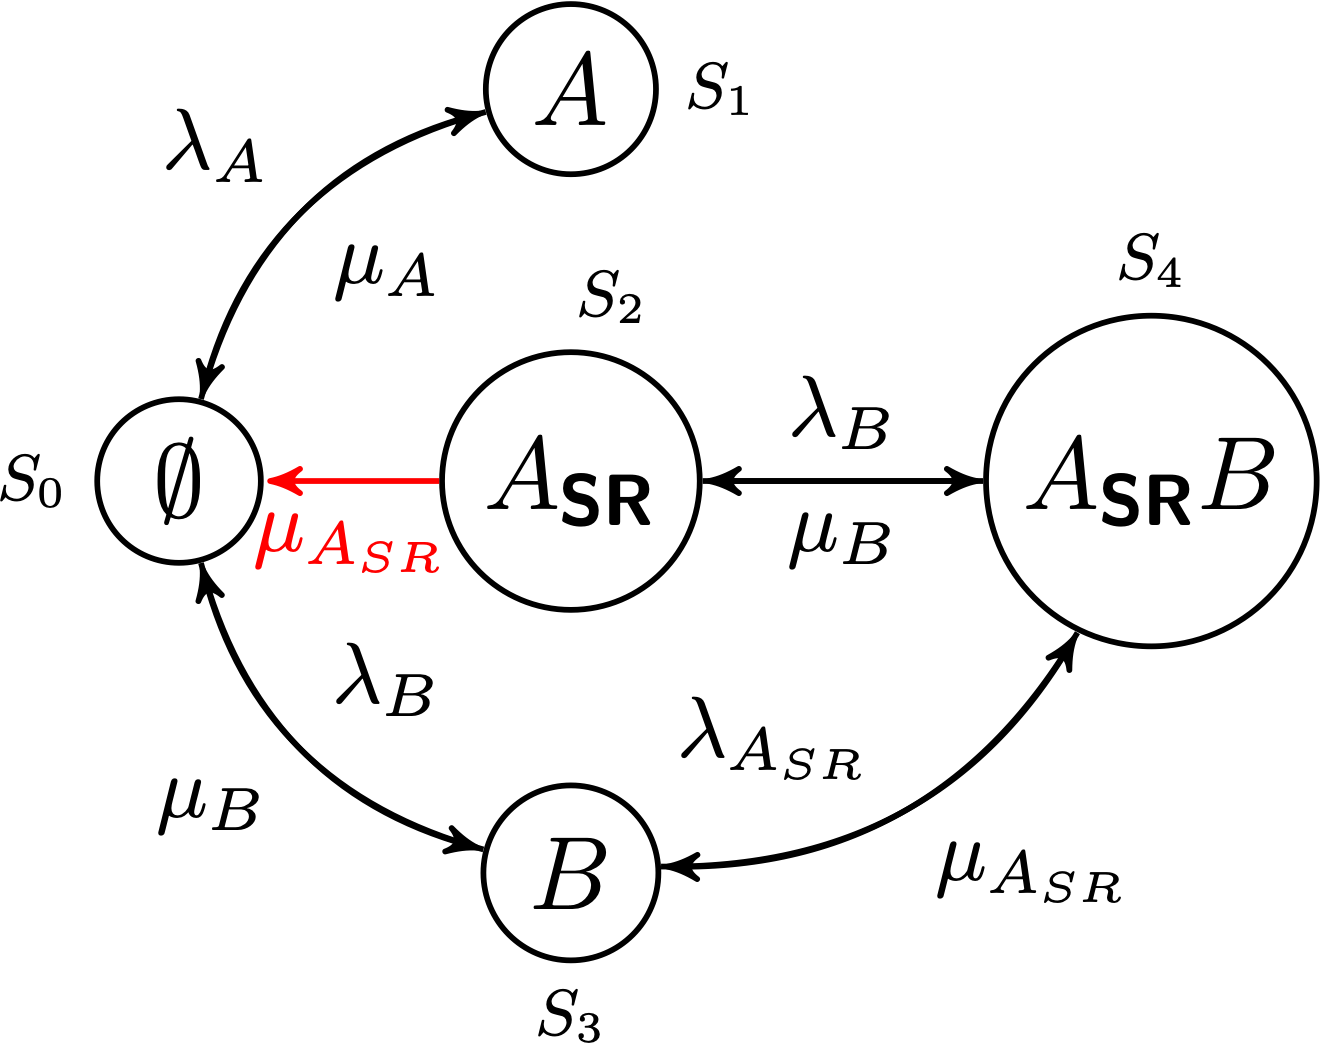
\includegraphics[width=0.47\textwidth]{images/ctmn_sr_2}}
	\caption{Example of the CTMN model for IEEE 802.11ax OBSS/PD-based SR.}
	\label{fig:model_11ax_sr}
\end{figure}

% 11be CSR
\subsection{IEEE 802.11be Coordinated Spatial Reuse}

To the date of publishing this thesis, the C-SR operation is currently being defined, studied, and characterized. However, we started devising its implications through the CTMN model. In particular, we have extended the 11ax-based model by taking the following assumptions:
\begin{enumerate}
	\item Coordinated transmissions always have priority when defining transitions between states. This means that joint transmission will occur over individual ones. 
	%
	\item The feasibility of a coordinated transmission is only assessed from the perspective of the sharing AP. Therefore, it is not assessed whether the transmission of shared APs will fail or succeed in transiting to coordinated states. 
	%
	\item Sharing and shared transmission duration are assumed to be equal.
\end{enumerate}

The C-SR operation through CTMNs is exemplified in Figure \ref{fig:model_11be_csr}. We address a deployment in which flow-in-the-middle starvation is prone to occur in a 3-BSS deployment if applying the default channel sensing mechanisms. As shown in Figure \ref{fig:ctmn_csr_1}, AP$_B$ would mark the channel as busy when detecting transmissions from either AP$_A$ or AP$_C$. However, AP$_A$ and AP$_C$ are not in range of each other and can, therefore, transmit simultaneously. The C-SR operation can solve the flow-in-the-middle situation. BSS$_A$ and BSS$_B$ can be coordinated to transmit simultaneously, thus leading to the new kind of inter-BSS interactions depicted in \ref{fig:ctmn_csr_2}. As shown, the introduced coordinated transmissions entail new inter-BSS interactions, which is, for instance, the simultaneous transmission of all the BSSs in the state $AB_{SR}C$. Similarly to 11ax OBSS/PD-based SR, the coordinated transmission requires adjusting the transmit power in order not to affect the primary transmissions (i.e., the ones started by the sharing nodes). In this case, the transmit power of both sharing and shared APs is negotiated based on the DL ARIL of the intended receivers. The fact of keeping track of the interference support by each STA allows improving further the quality of the transmissions resulting from the SR operation.

\begin{figure}[ht!]
	\centering
	\subfigure[Deployment]{\label{fig:ctmn_csr_1}\raisebox{6mm}{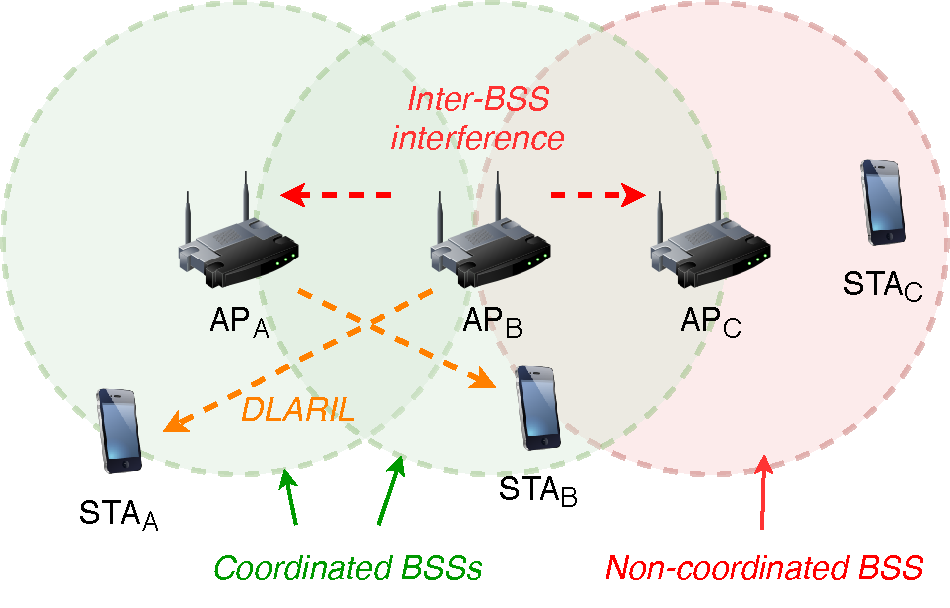
\includegraphics[width=0.45\textwidth]{images/ctmn_csr_1}}} % 
	\subfigure[CTMN]{\label{fig:ctmn_csr_2}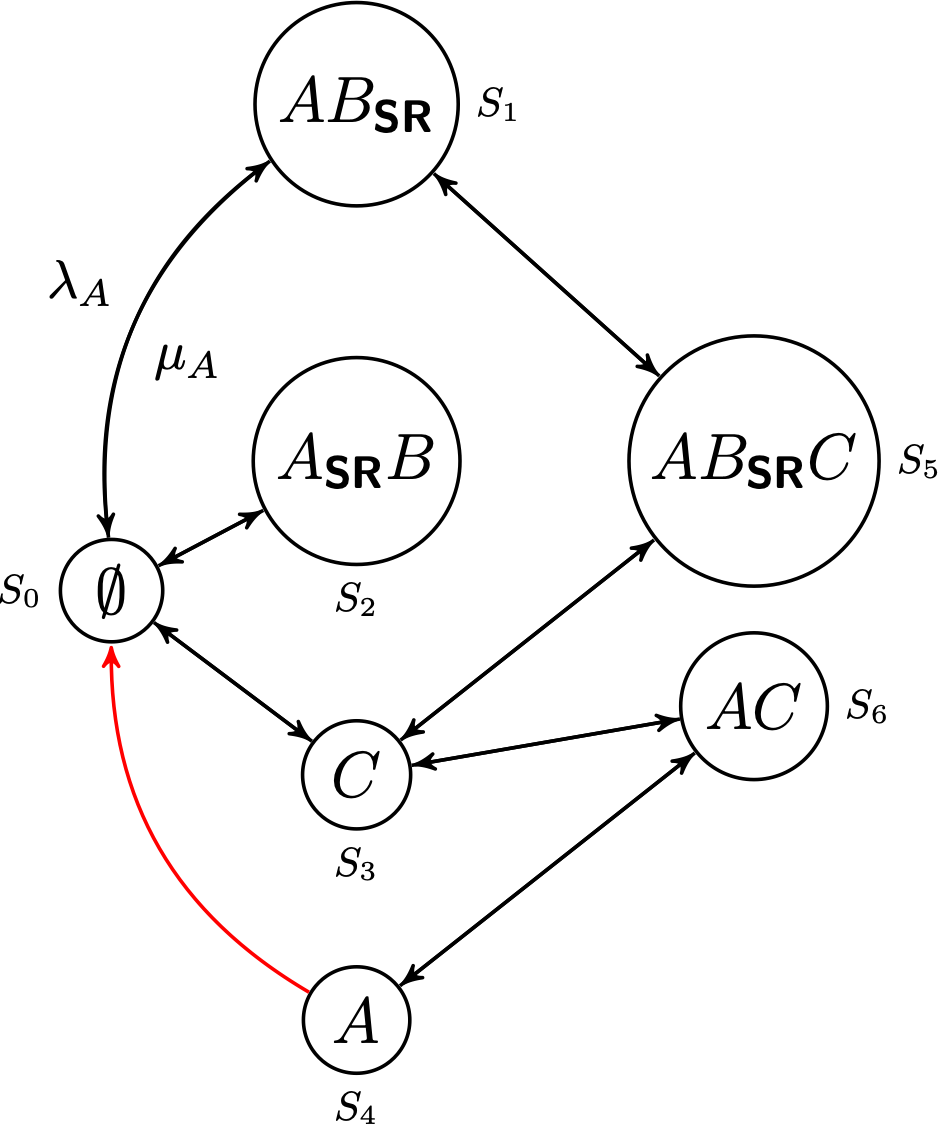
\includegraphics[width=0.35\textwidth]{images/ctmn_csr_2}}
	\caption{Example of the CTMN model for IEEE 802.11be C-SR.}
	\label{fig:model_11be_csr}
\end{figure}

% Simulation
\section{Simulation of Sequential Learning for Spatial Reuse}
\label{section_4_2}

\subsection{Spatial Reuse Implementation}

To devise the potential gains that SR can provide to next-generation dense wireless networks, we introduce the 11ax SR operation in the Komondor simulator, which is presented in \textbf{Paper \#4}. Komondor has been conceived to \emph{i)} allow the low-cost integration of novel mechanisms included in new IEEE 802.11 standards, \emph{ii)} simulate high-dense deployments, and \emph{iii)}  include the operation of sequential learning algorithms within the simulation of the network.

% Komondor details
To characterize the operation of WLANs in a realistic manner, Komondor reproduces actual transmissions on a per-packet basis. To that purpose, Komondor is based on the COST library, which allows building interactions between components (e.g., wireless nodes, buffers, packets) through synchronous and asynchronous events. The implementation of DCF in Komondor has been validated against ns-3, and the CTMN \cite{bellalta2014throughput} and Bianchi models \cite{bianchi2000performance}.

For 11ax OBSS/PD-based SR, the behavior of Komondor is as follows (also illustrated in Figure \ref{fig:komondor_sr}):
\begin{itemize}
	\item Devices implementing SR must announce that they support the operation so that devices in a BSS are setup. 
	\item On initiating an SR-enabled transmission, a device must indicate its BSS Color and SRG.
	\item Overlapping devices implementing SR, can take advantage of SR-enabled transmissions and transmit concurrently. The following conditions must hold for any detected transmission (i.e., the received power is above the minimum CCA/CS threshold):
	\begin{itemize}
		\item Detected transmissions must indicate support for SR.
		\item Detected transmissions belong to different BSS Color sets or SRGs than the device detecting SR-based transmission opportunities. 
		\item The power detected from the transmission must not exceed the assigned OBSS/PD threshold.
		\item The transmit power to be used in the concurrent transmission must be limited according to the SR rules (see Chapter \ref{chapter2}).
	\end{itemize}
	\item In case of not meeting the abovementioned requirements, it is not possible to transmit during the SR TXOP, so the device activates a NAV timer.
\end{itemize}

\begin{figure}[ht!]
	\centering
	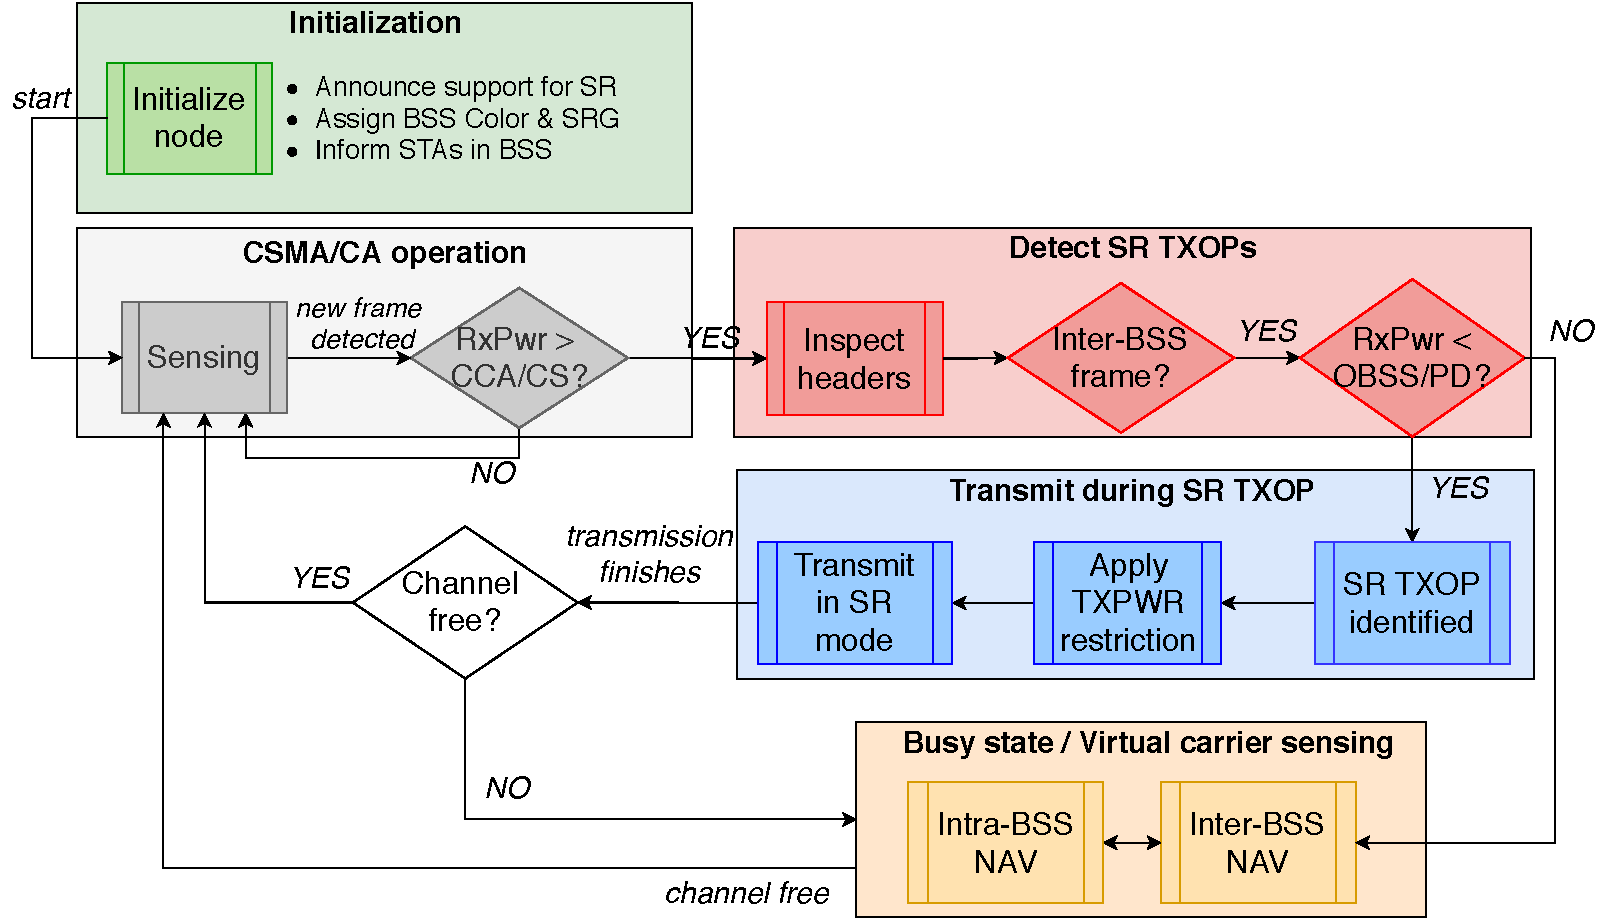
\includegraphics[width=.9\textwidth]{images/komondor_sr}
	\caption{Implementation of IEEE 802.11ax OBSS/PD-based SR in Komondor.}
	\label{fig:komondor_sr}
\end{figure}

% Related work
The IEEE 802.11ax SR operation has also been developed for ns-3, but it has been published very recently\footnote{\url{https://gitlab.com/nsnam/ns-3-dev/-/tags/ns-3.30}}. In particular, we provided the implementation in Komondor as a complementary way to characterize and understand SR. Notice that ns-3 includes an exhaustive model of the physical (PHY) layer, whereas the primary goal of this thesis lies in the MAC interactions occurring when using SR. Related to this, the lower complexity of Komondor allows us to simulate high-density deployments with reasonable simulation times. Apart from that, Komondor continues providing extended features of 11ax SR. The ns-3 implementation includes baseline OBSS/PD-based SR with constant thresholds. In contrast, Komondor allows us to easily introduce algorithms to adjust the OBSS/PD threshold dynamically. Besides, the implementation of SRGs is provided to explore its potential utilization in future IEEE 802.11 amendments. 

\subsection{Agents-based Implementation}
% ML in Komondor
Regarding the integration of ML mechanisms into network simulation, we find the integration of AI Gym with ns-3 \cite{gawlowicz2019ns}, which provides a discrete interaction between the simulated network components and AI libraries. When it comes to Komondor, a fully integrated implementation of agents was provided. These agents interact with simulated nodes in a network for providing monitoring, processing, and decision-making functionalities. In particular, different communication-based approaches are considered to enable the application of decentralized, distributed, centralized, and hybrid ML mechanisms (see Figure \ref{fig:overview_agents}).
\begin{figure}[ht!]
	\centering
	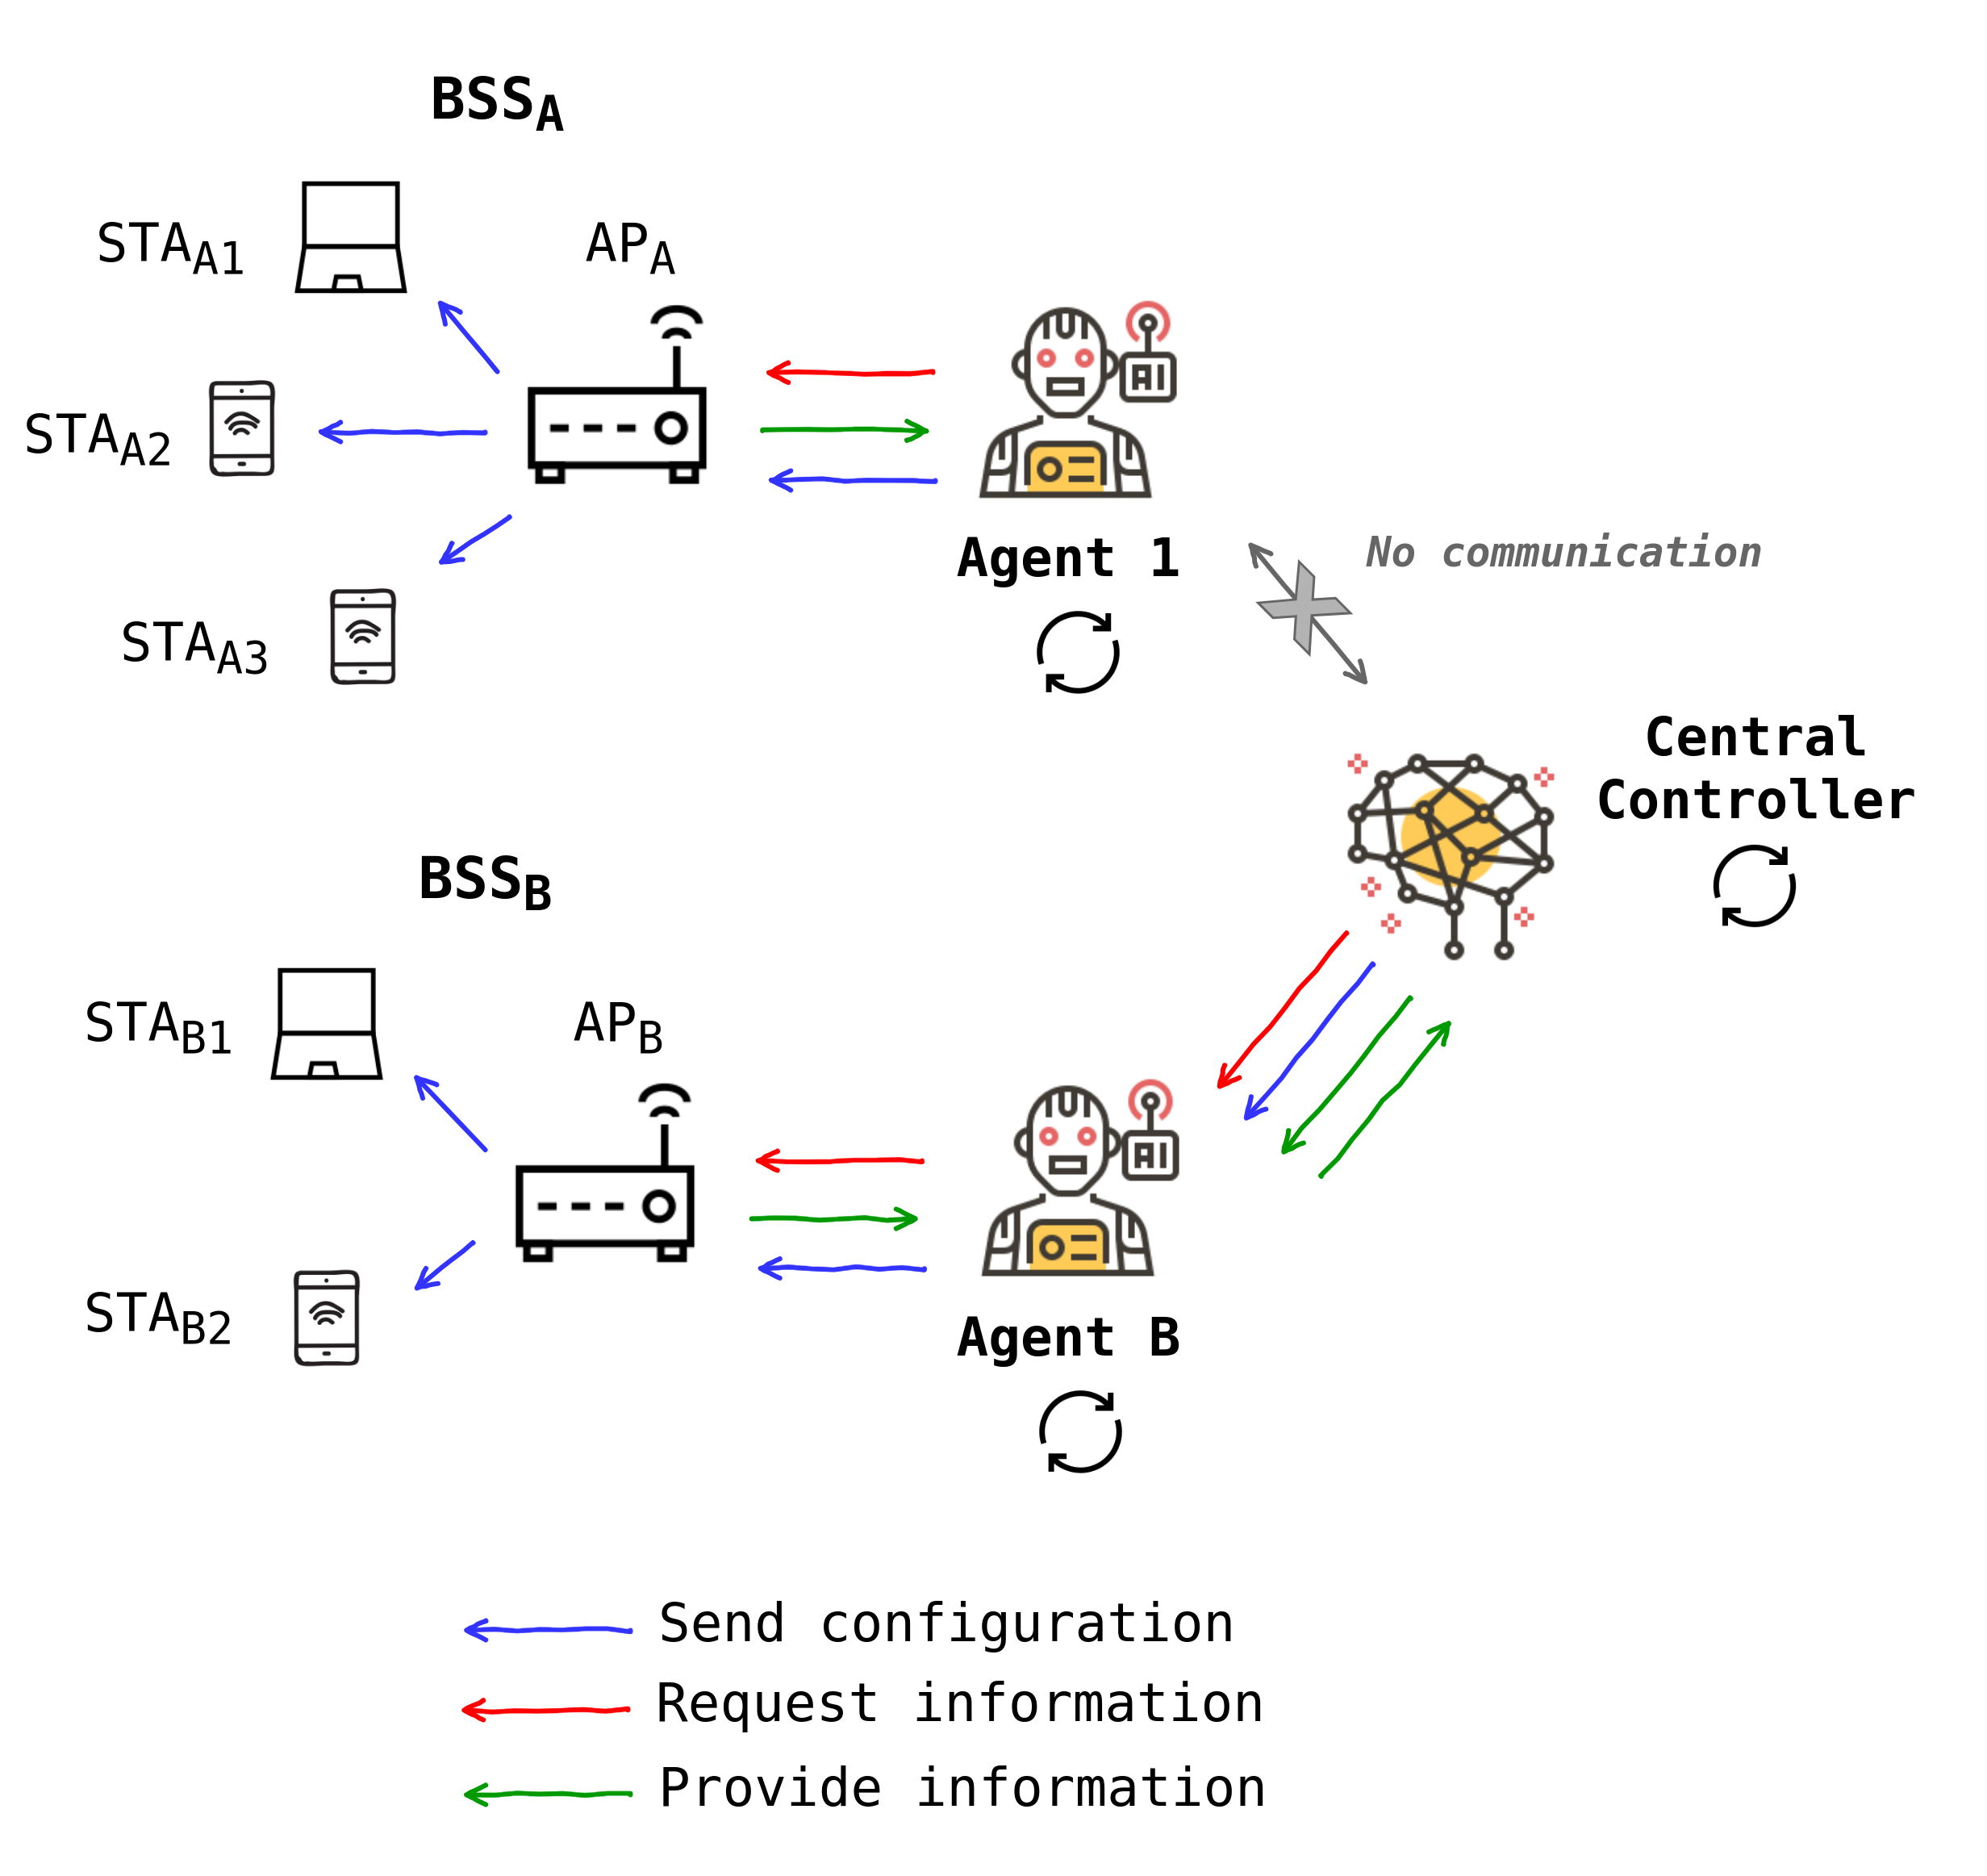
\includegraphics[width=.7\textwidth]{images/overview_agents}
	\caption{Agents implementation in Komondor.}
	\label{fig:overview_agents}
\end{figure}

On designing sequential learning mechanisms in Komondor, the following considerations should be taken into account:
\begin{itemize}
	\item Agents acquire information from BSSs on a periodical-basis. The information retrieval interval depends on the established monitoring phase, which entails a trade-off between the delay in making decisions and the quality of the sample extracted from monitoring.
	\item The information acquired by agents can be later shared among other BSSs or with a centralized entity, thus allowing to build cooperative, distributed, or centralized mechanisms. Agents with different purposes can coexist.
	\item The communication among agents and APs can be assumed to be virtual or entail certain costs (e.g., delay, overhead). Besides, packet losses can be included when agents exchange information, which can impact on the learning procedure followed by agents.
\end{itemize} 

%%%%%%%%%%%%%%%%%
% RESULTS
%%%%%%%%%%%%%%%%%
\chapter{Main Findings}
\label{chapter5}

In this Chapter, we present the main findings of this dissertation, which result from the analysis of the 11ax SR operation and the application of ML to address SR. \textbf{Paper \#5} and \textbf{Paper \#6} focus on the model, characterization, and analysis of IEEE 802.11 SR, thus aiming to show the potential achievable gains of this technology. Then, \textbf{Paper \#1}, \textbf{Paper \#2} and \textbf{Paper \#3} study the applicability of sequential learning for SR through different proposed mechanisms. Specifically, \textbf{Paper \#1} proposes a multi-agent setting in which players implement a stateless version of Q-learning \cite{sutton2018reinforcement, watkins1992q} to optimize a selfish reward based on the local throughput. Similarly, \textbf{Paper \#2} and \textbf{Paper \#3} propose the utilization of MABs for addressing the multi-agent SR problem. While \textbf{Paper \#2} analyzes the impact of different algorithms ($\varepsilon$-greedy, EXP3, UCB, and Thompson sampling) in selfish settings, \textbf{Paper \#3} extends the analysis to collaborative rewards. Finally, \textbf{Paper \#6}, \textbf{Paper \#7}, and \textbf{Paper \#8} delve into the necessary infrastructure and tools to carry out the main object of study of this thesis.

%\section{Performance gains of IEEE 802.11ax Spatial Reuse}
\begin{tcolorbox}
		\textbf{Finding \#1:} SR is a fair mechanism that allows increasing the number of simultaneous transmissions in dense OBSSs, thus enhancing the throughput in high-interference scenarios.
\end{tcolorbox}

The analysis of 11ax SR has been conducted in \textbf{Paper \#5} and \textbf{Paper \#6} for residential and enterprise-like Wi-Fi deployments (see Figure \ref{fig:random_scenario}). Our results compare the legacy setting (CCA/CS is used for all the transmissions) to SR with the best OBSS/PD threshold. In the first place, Figure \ref{fig:paper_1_throughput} shows the throughput experienced by the BSSs in an overlapping deployment for different network densities and traffic load values. Solid bars refer to the performance achieved by the BSS implementing SR, while dashed bars are for the rest of overlapping BSSs. The first important conclusion is that SR is a fair mechanism that protects the detected legacy transmissions to transmit in SR mode. Notice that the performance of BSSs that are not applying SR (dashed bars) is barely affected when SR is applied by other BSSs (solid bars). Besides, BSSs applying SR can overcome high-interference settings that lead to suffering starvation and other performance anomalies (e.g., collisions). Accordingly, the throughput of dense deployments is improved.

\begin{figure}[ht!]
	\centering
	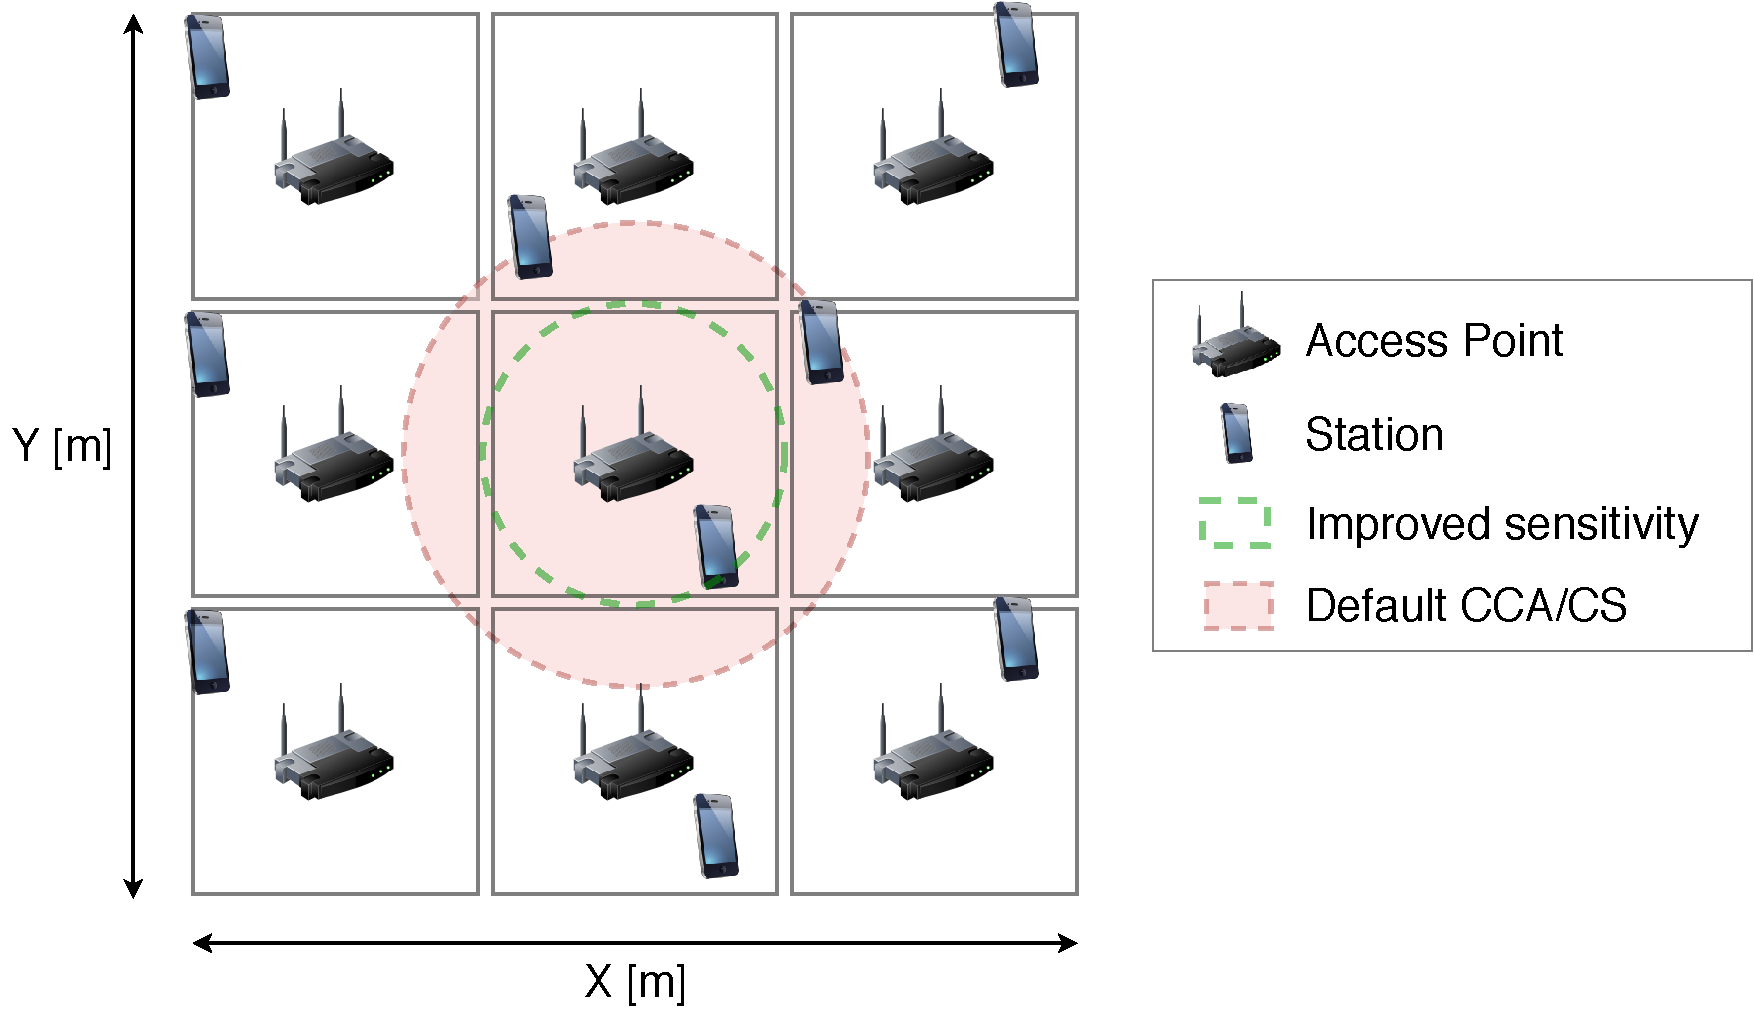
\includegraphics[width=0.6\textwidth]{images/random_scenario}
	\caption{Residential and enterprise-like deployments to evaluate the performance gains of IEEE 802.11ax Spatial Reuse.}
	\label{fig:random_scenario}
\end{figure}

\begin{figure}[ht!]
	\centering
	\subfigure[Network density]{\label{fig:paper_1_throughput_per_density}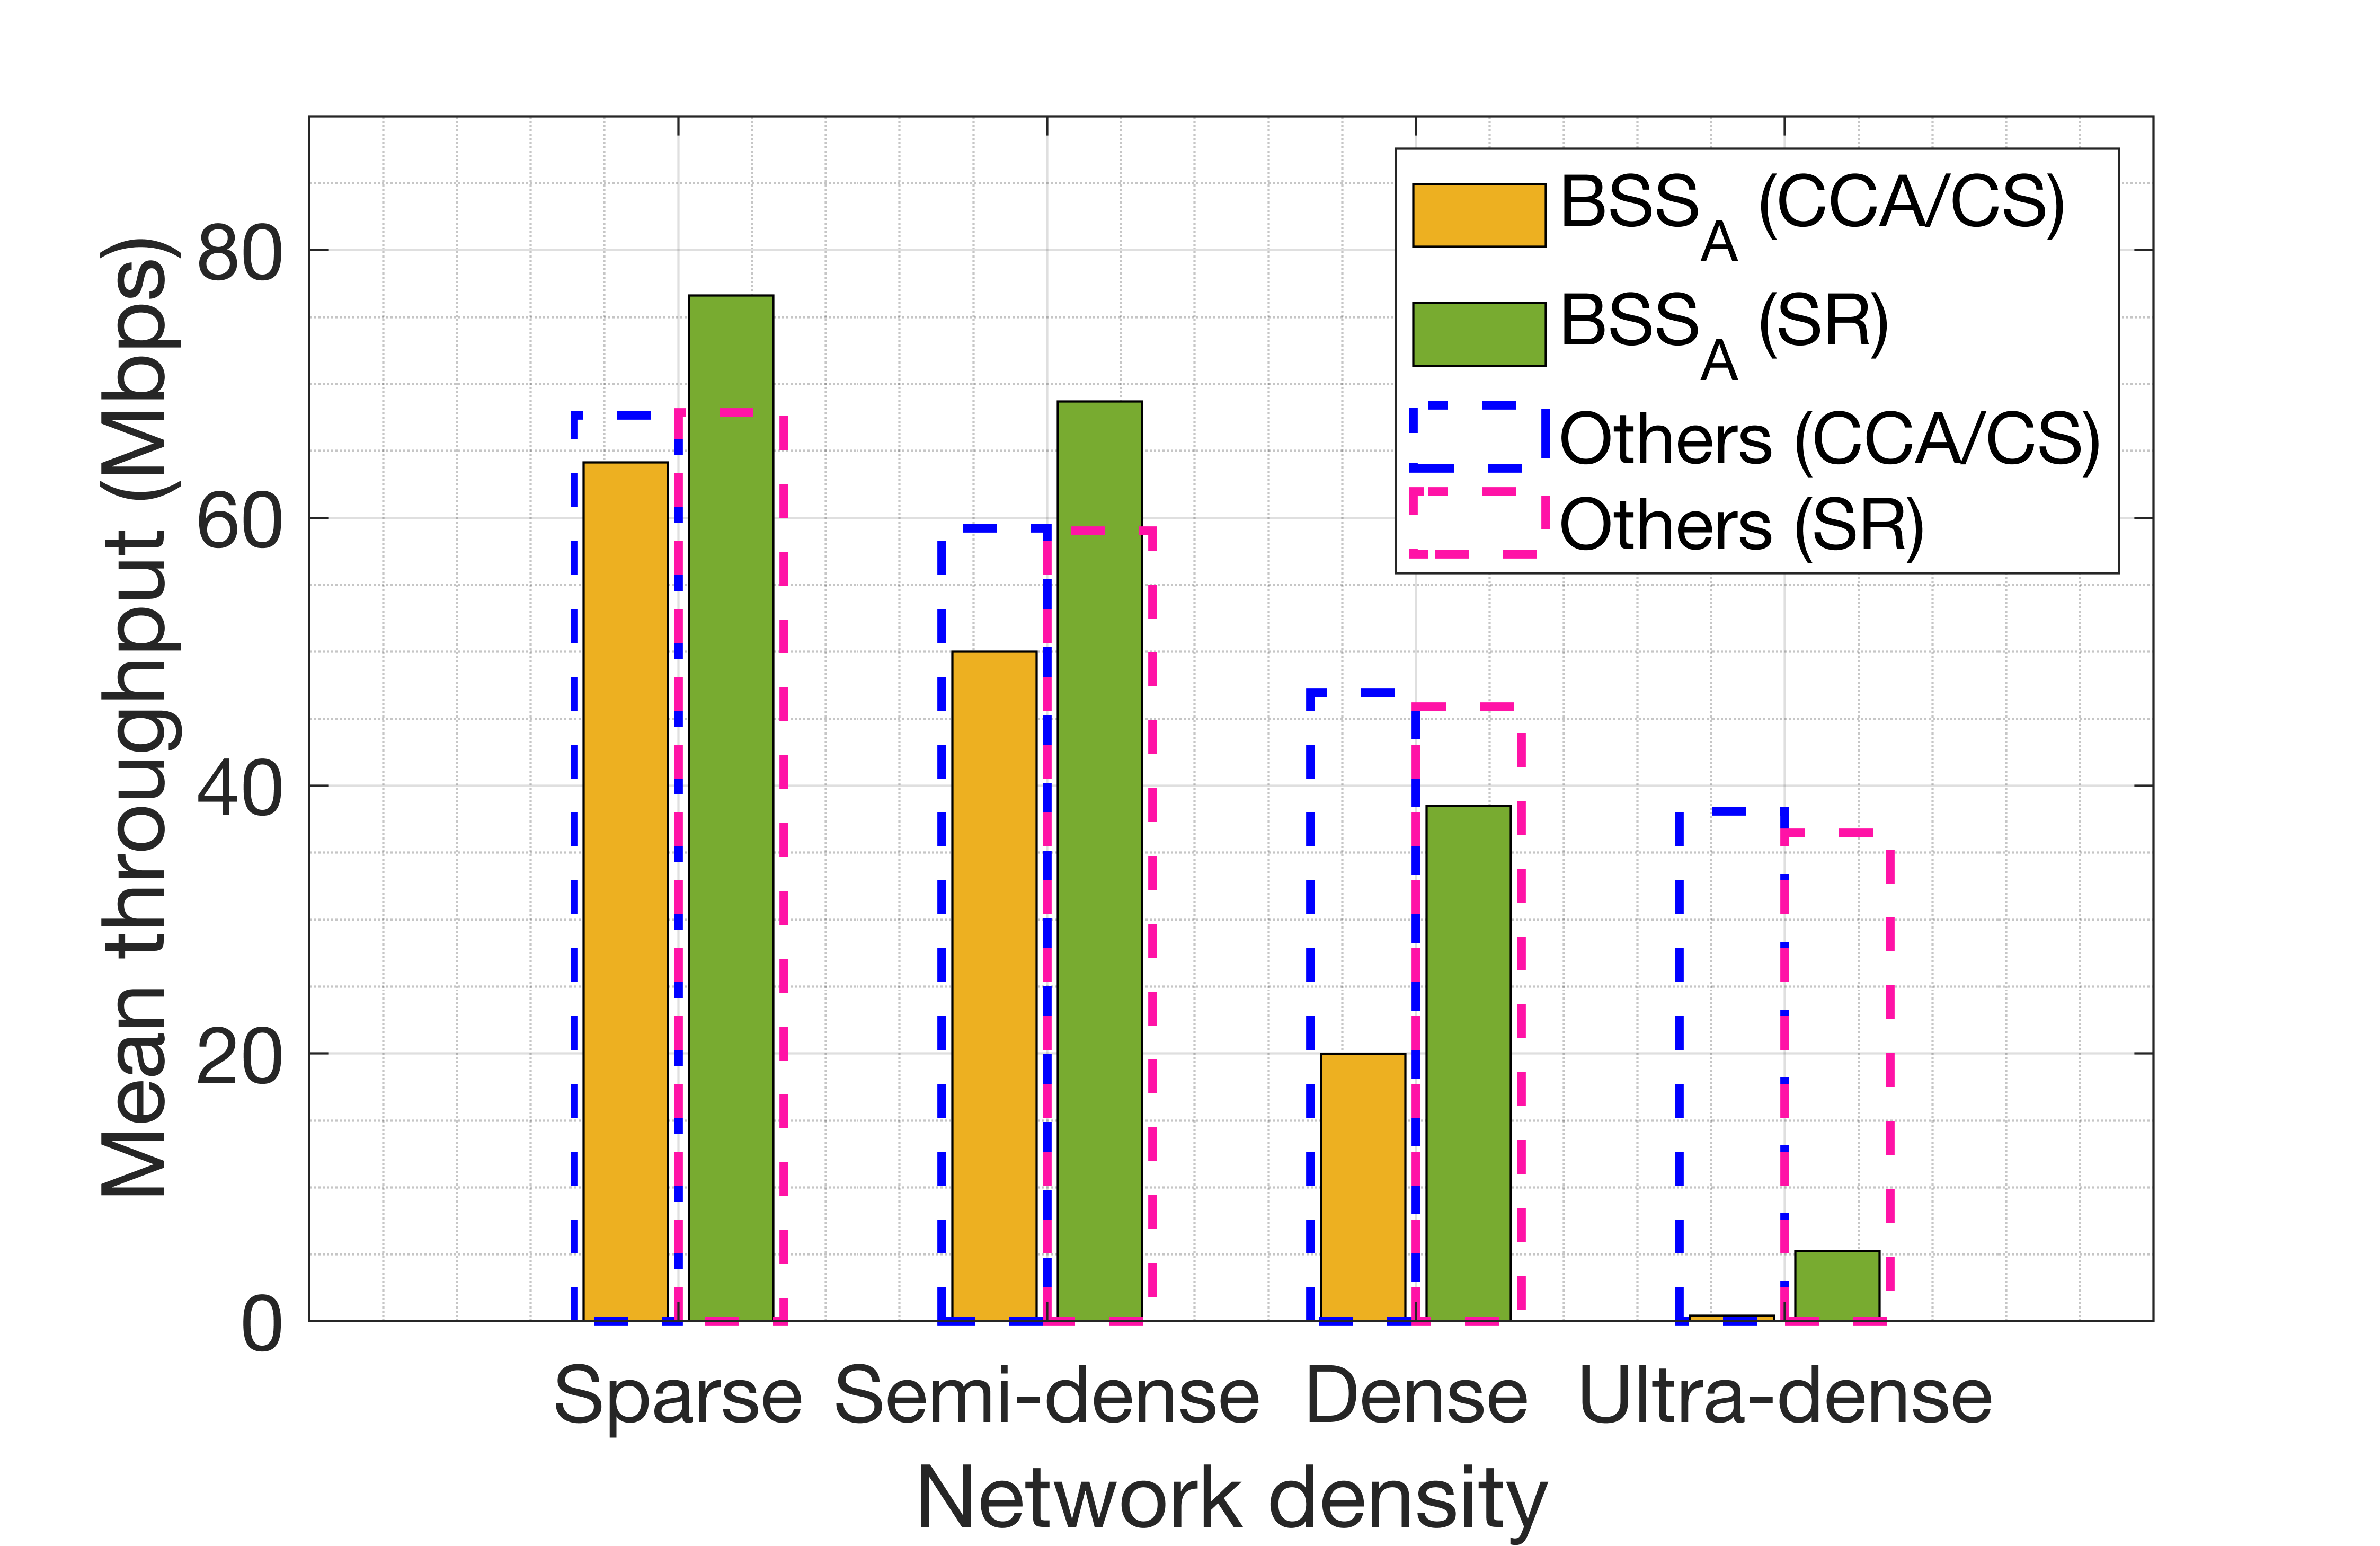
\includegraphics[width=0.43\textwidth]{images/paper_1_throughput_per_density}}
	\subfigure[Traffic load]{\label{fig:paper_1_throughput_per_load}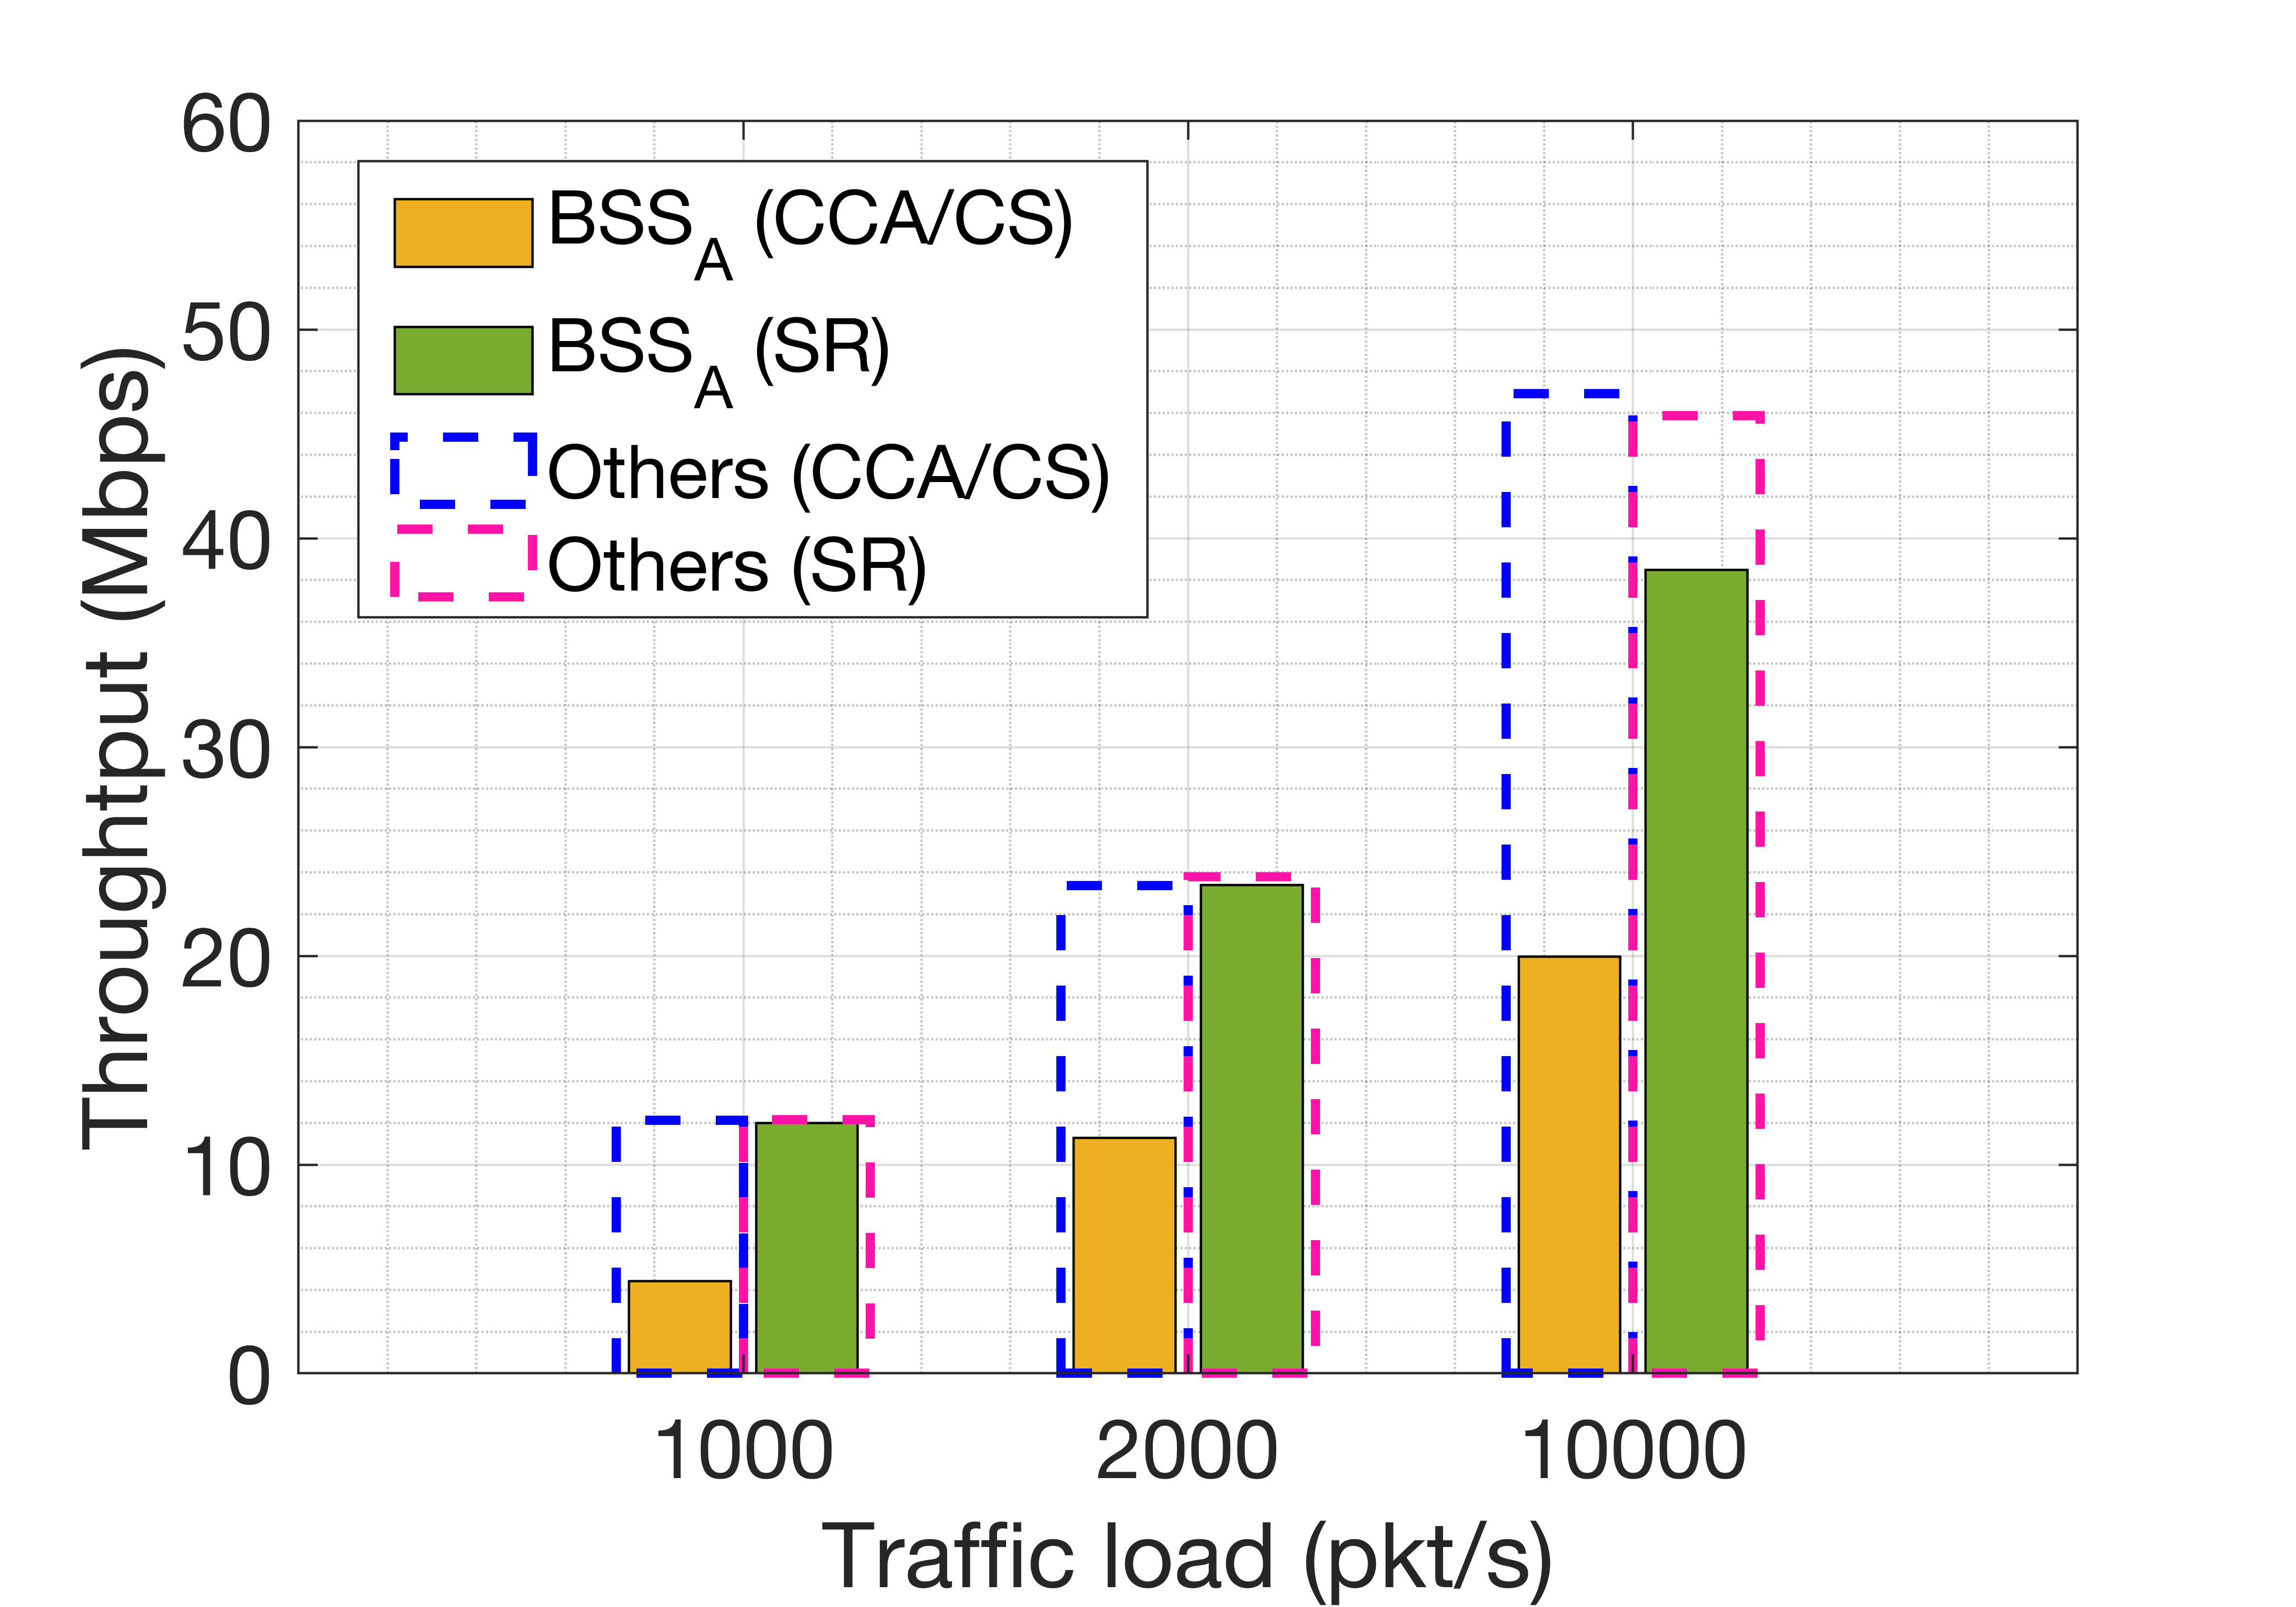
\includegraphics[width=0.4\textwidth]{images/paper_1_throughput_per_load}}
	\caption{Throughput gains obtained by IEEE 802.11ax Spatial Reuse in comparison to default carrier sensing approaches. Different network densities and traffic load values have been considered.}
	\label{fig:paper_1_throughput}
\end{figure}

\begin{tcolorbox}
	\textbf{Finding \#2:} SR allows to significantly improve the delay in dense deployments. 
\end{tcolorbox}

This finding is illustrated in Figure \ref{fig:paper_2_delay}, which shows the CDF of the delay for different network densities and traffic load values. As for the throughput evaluation, solid lines refer to the performance achieved by the BSS implementing SR, while dashed lines are for the rest of overlapping BSSs. As illustrated, the probability of experiencing a high delay increases rapidly with the traffic load and the deployment's density. Nevertheless, the SR operation provides a substantial improvement in the delay, thus outperforming the legacy carrier sensing approach. The leading cause of this improvement lies in the number of simultaneous transmissions that are allowed through SR. \textbf{Paper \#5} and \textbf{Paper \#6} fully describe this finding.

\begin{figure}[ht!]
	\centering
	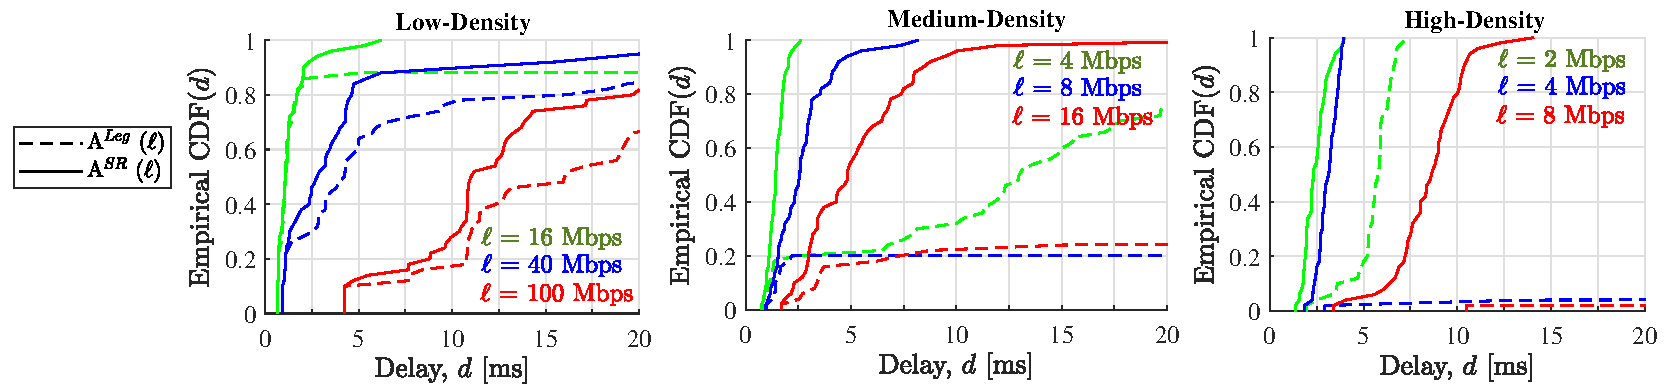
\includegraphics[width=\textwidth]{images/paper_2_delay}
	\caption{CDF of the delay gains obtained by IEEE 802.11ax Spatial Reuse in comparison to default carrier sensing approaches. Different network densities and traffic load values have been considered.}
	\label{fig:paper_2_delay}
\end{figure}

\begin{tcolorbox}
	\textbf{Finding \#3:} The lack of coordination of the IEEE 802.11ax SR mechanism prevents providing further performance gains in dense deployments.
\end{tcolorbox}
Although SR has been shown to enhance current IEEE 802.11ax deployments, its performance is bounded by the following characteristics: 
\begin{itemize}
	\item The current transmit power limitation is too conservative, and further gains are expected if it is properly adjusted by BSSs participating in SR-based transmissions.
	\item The lack of coordination among BSSs implementing SR prevents to find the optimal scheduling allocations. Through coordinated transmissions, BSSs can determine the optimal set of transmitter-receiver nodes in each SR-based transmission.
	\item The rigidity of the current approach, which is applied homogeneously in a BSS instead of considering per-STA behavior.
	\item SR is not combined with other technologies such as OFDMA or beamforming, which is expected to provide further performance gains. 
\end{itemize}
\textbf{Paper \#5} and \textbf{Paper \#6} give some insights regarding this finding. Apart from that, in Figure \ref{fig:performance_csr}, we devise the potential gains provided by CSR in comparison to the default carrier sensing approach and the 11ax OBSS/PD-based SR operation. Notice that the obtained results are preliminary since the CSR is currently under study and is part of the future work. In particular, we study the effect of coordination in a simple deployment with two BSSs, namely BSS$_A$ and BSS$_B$. As illustrated, the fact of coordinating the transmissions held between the devices in BSS$_A$ and BSS$_B$ allows improving the transmit power used in each case, thus granting a higher throughput. 

\begin{figure}[ht!]
	\centering
	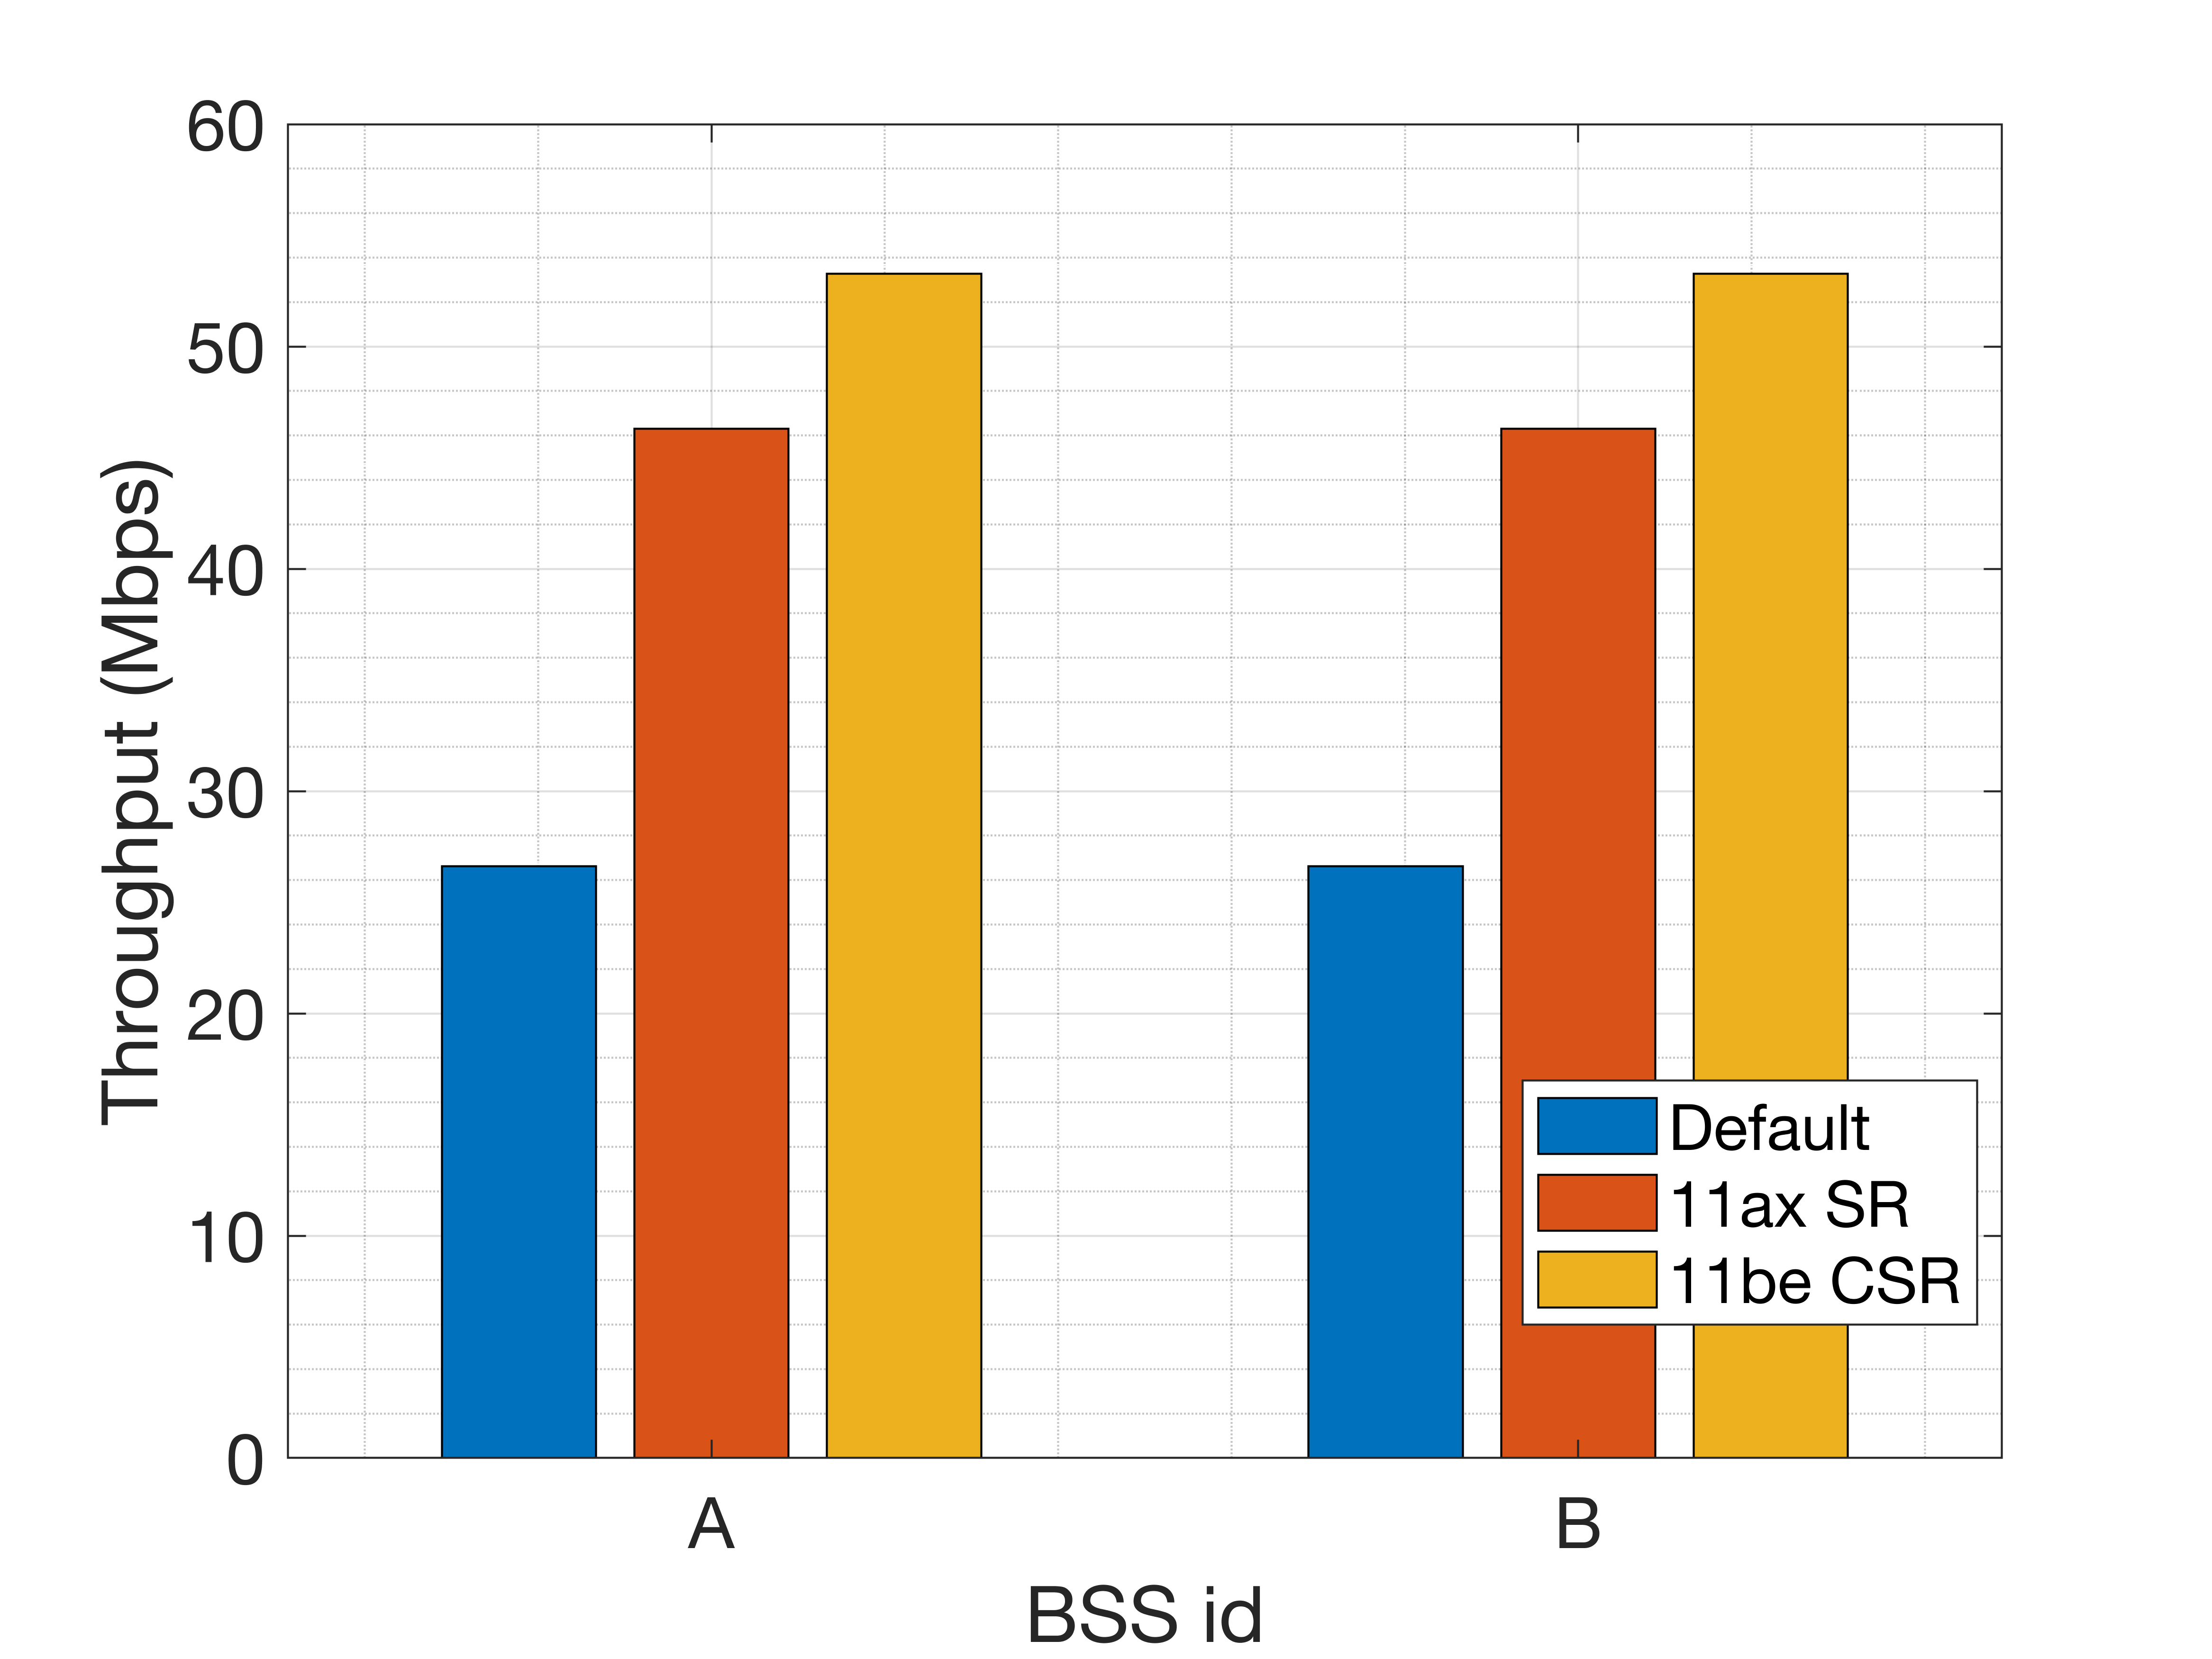
\includegraphics[width=.5\textwidth]{images/performance_csr}
	\caption{Further SR gains provided by CSR in comparison to default carrier sensing and OBSS/PD-based SR.}
	\label{fig:performance_csr}
\end{figure}
 
 %\section{Machine Learning for Spatial Reuse}
\begin{tcolorbox}
	\textbf{Finding \#4:} Sequential learning mechanisms for multi-agent SR allow improving the performance of WLANs but may fail at finding a global optimum due to the competition among BSSs.
\end{tcolorbox} 

To address the SR problem in decentralized WLANs, we proposed the application of different multi-player sequential learning approaches, which vary according to the available information that agents have about the surrounding environment (i.e., other players). 

In \textbf{Papers \#1} and \textbf{Paper \#2}, we studied the effects of using selfish rewards (local information only) in competitive settings where multiple agents coexist. We showed that the concurrent learning operation may lead to a competitive setting, which has an impact on the learning procedure carried out by each agent. In particular, the joint learning operation was shown to prevent finding the optimal global configuration and potentially leading to a high variability on the rewards obtained by each agent (intermittent good/poor performance depending on the neighbor decisions). These effects were shown to be motivated by the throughput demands of individual agents, making the global function highly non-convex. In turn, the selfish setting was also shown to boost fairness in some situations. This is the case where the global optimum solution, which depends on each agent (e.g., location, set of available configurations), favors collaboration among BSSs, even if individual rewards are selfish.

The effects of learning SR selfishly in a multi-player setting are summarized in Figure \ref{fig:temporal_individual_tpt_TS}, which shows the throughput evolution of four BSSs that apply sequential learning for tuning both the sensitivity and the transmit power. As shown, the concurrent learning operation prevents reaching the optimal individual performance (depicted by the red dashed line). Regarding stability aspects, we noticed that the provided algorithms converged slowly to a stable configuration. Nevertheless, the learning procedure is characterized by a high throughput variability. The main cause lies in the competitive setting, whereby agents intermittently select good/bad performing actions. In practice, agents end up picking a protective configuration that prevents to reach the global optimum. The variability issues that arise from this kind of multi-agent deployments can be mitigated from an implementation point of view (e.g., define stop goals, enforce mechanisms for convergence, reduce the learning rate, etc.).   

\begin{figure*}[ht!]
	\centering
	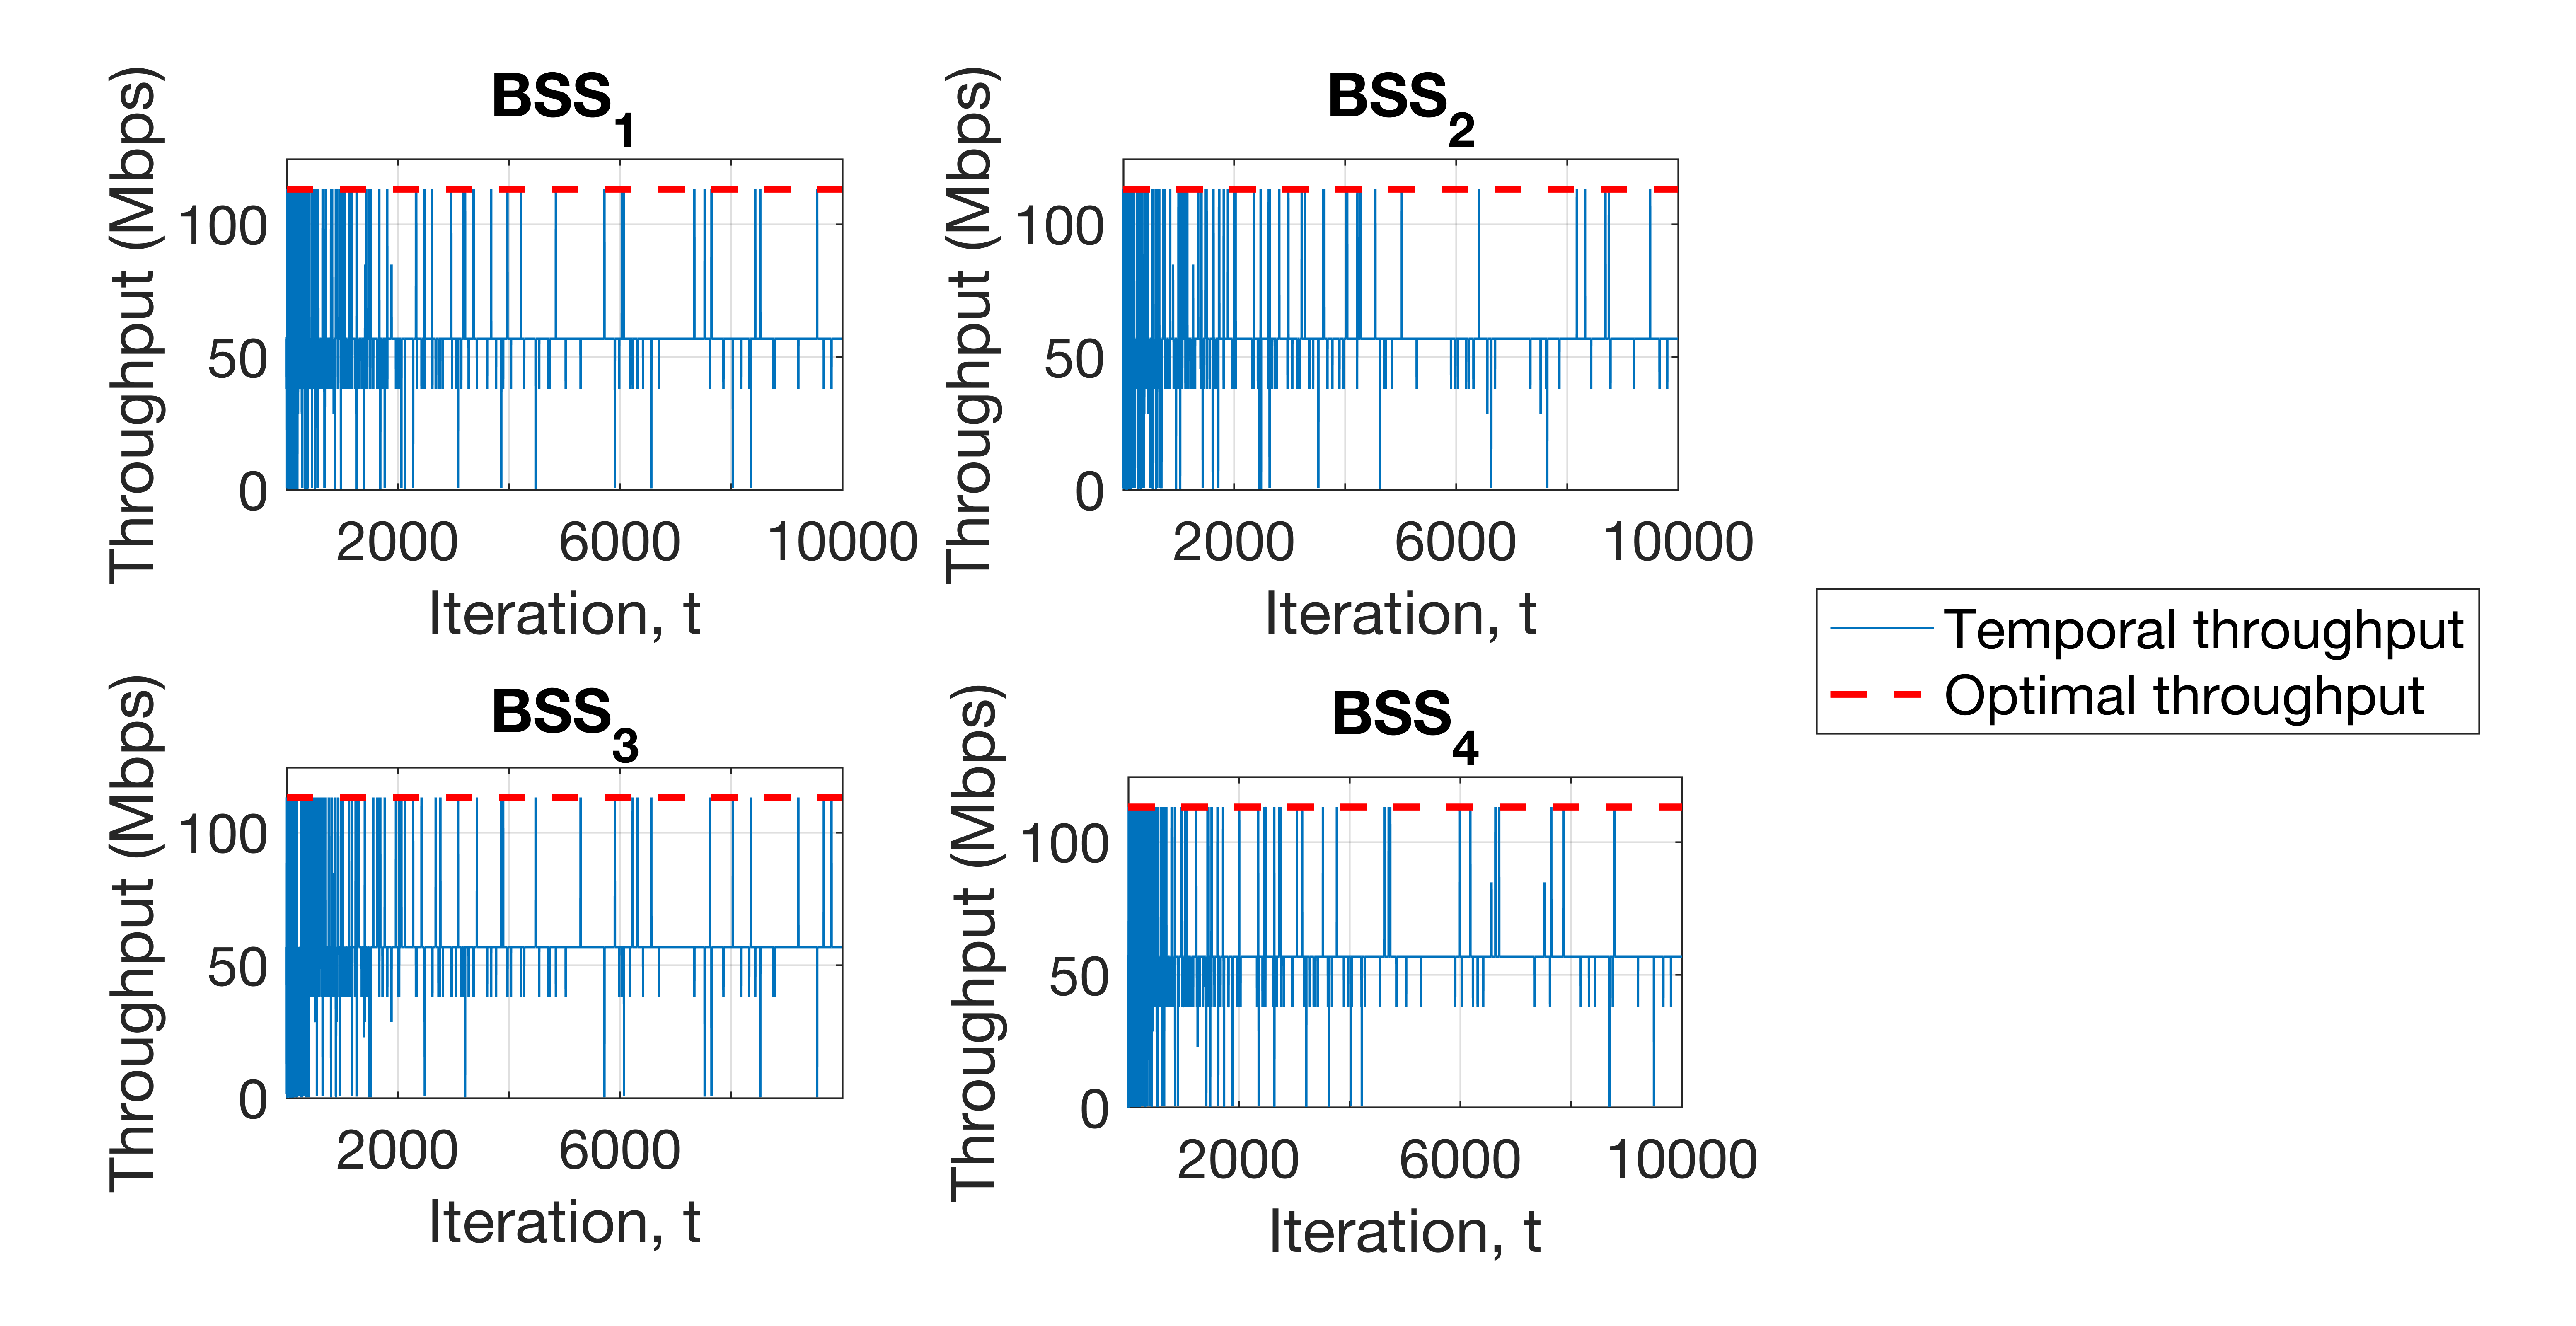
\includegraphics[width=0.5\textwidth]{images/temporal_individual_tpt_TS}
	\caption{Implications of learning SR selfishly in a multi-player setting.}
	\label{fig:temporal_individual_tpt_TS}
\end{figure*}

\begin{tcolorbox}
	\textbf{Finding \#5:} Collaborative rewards enhance fairness in decentralized settings, but do not ensure reaching an optimal global solution.
\end{tcolorbox} 

In \textbf{Paper \#2}, we also studied the performance of collaborative settings, whereby the reward of an individual agent takes into consideration the performance of the other players. In this regard, we observed that collaborative rewards are useful to prevent unfairness, but face the same challenges as selfish approaches for converging to an optimal global solution. In the first place, each agent is responsible for its own action set but has no control on the joint action profile. Therefore, the action-selection procedure is kept decentralized. Otherwise, due to the combinatorial nature of the problem, the complexity would grow very fast. Apart from that, the global optimization function has multiple maximums, even if it is based on a collaborative metric.

To illustrate the effect of using cooperative rewards in a multi-player setting, Figure \ref{fig:paper_5_scalability} shows the average throughput and the max-min throughput obtained in random enterprise-like deployments, for different network densities. The default (static) configuration is compared to learning approaches based on non-cooperative (selfish) and cooperative (environment-aware) rewards. As illustrated, the cooperative reward allows improving fairness (shown in Figure \ref{fig:paper_5_scalability_mean_maxmin}), but leads to a lower overall performance if compared to the selfish mechanism (shown in Figure \ref{fig:paper_5_scalability_mean_tpt}). %\textcolor{red}{[To be addressed here: How robust is the approach to changes in the WLAN topology?]}

\begin{figure*}[ht!]
	\centering
	\subfigure[Average throughput]{\label{fig:paper_5_scalability_mean_tpt}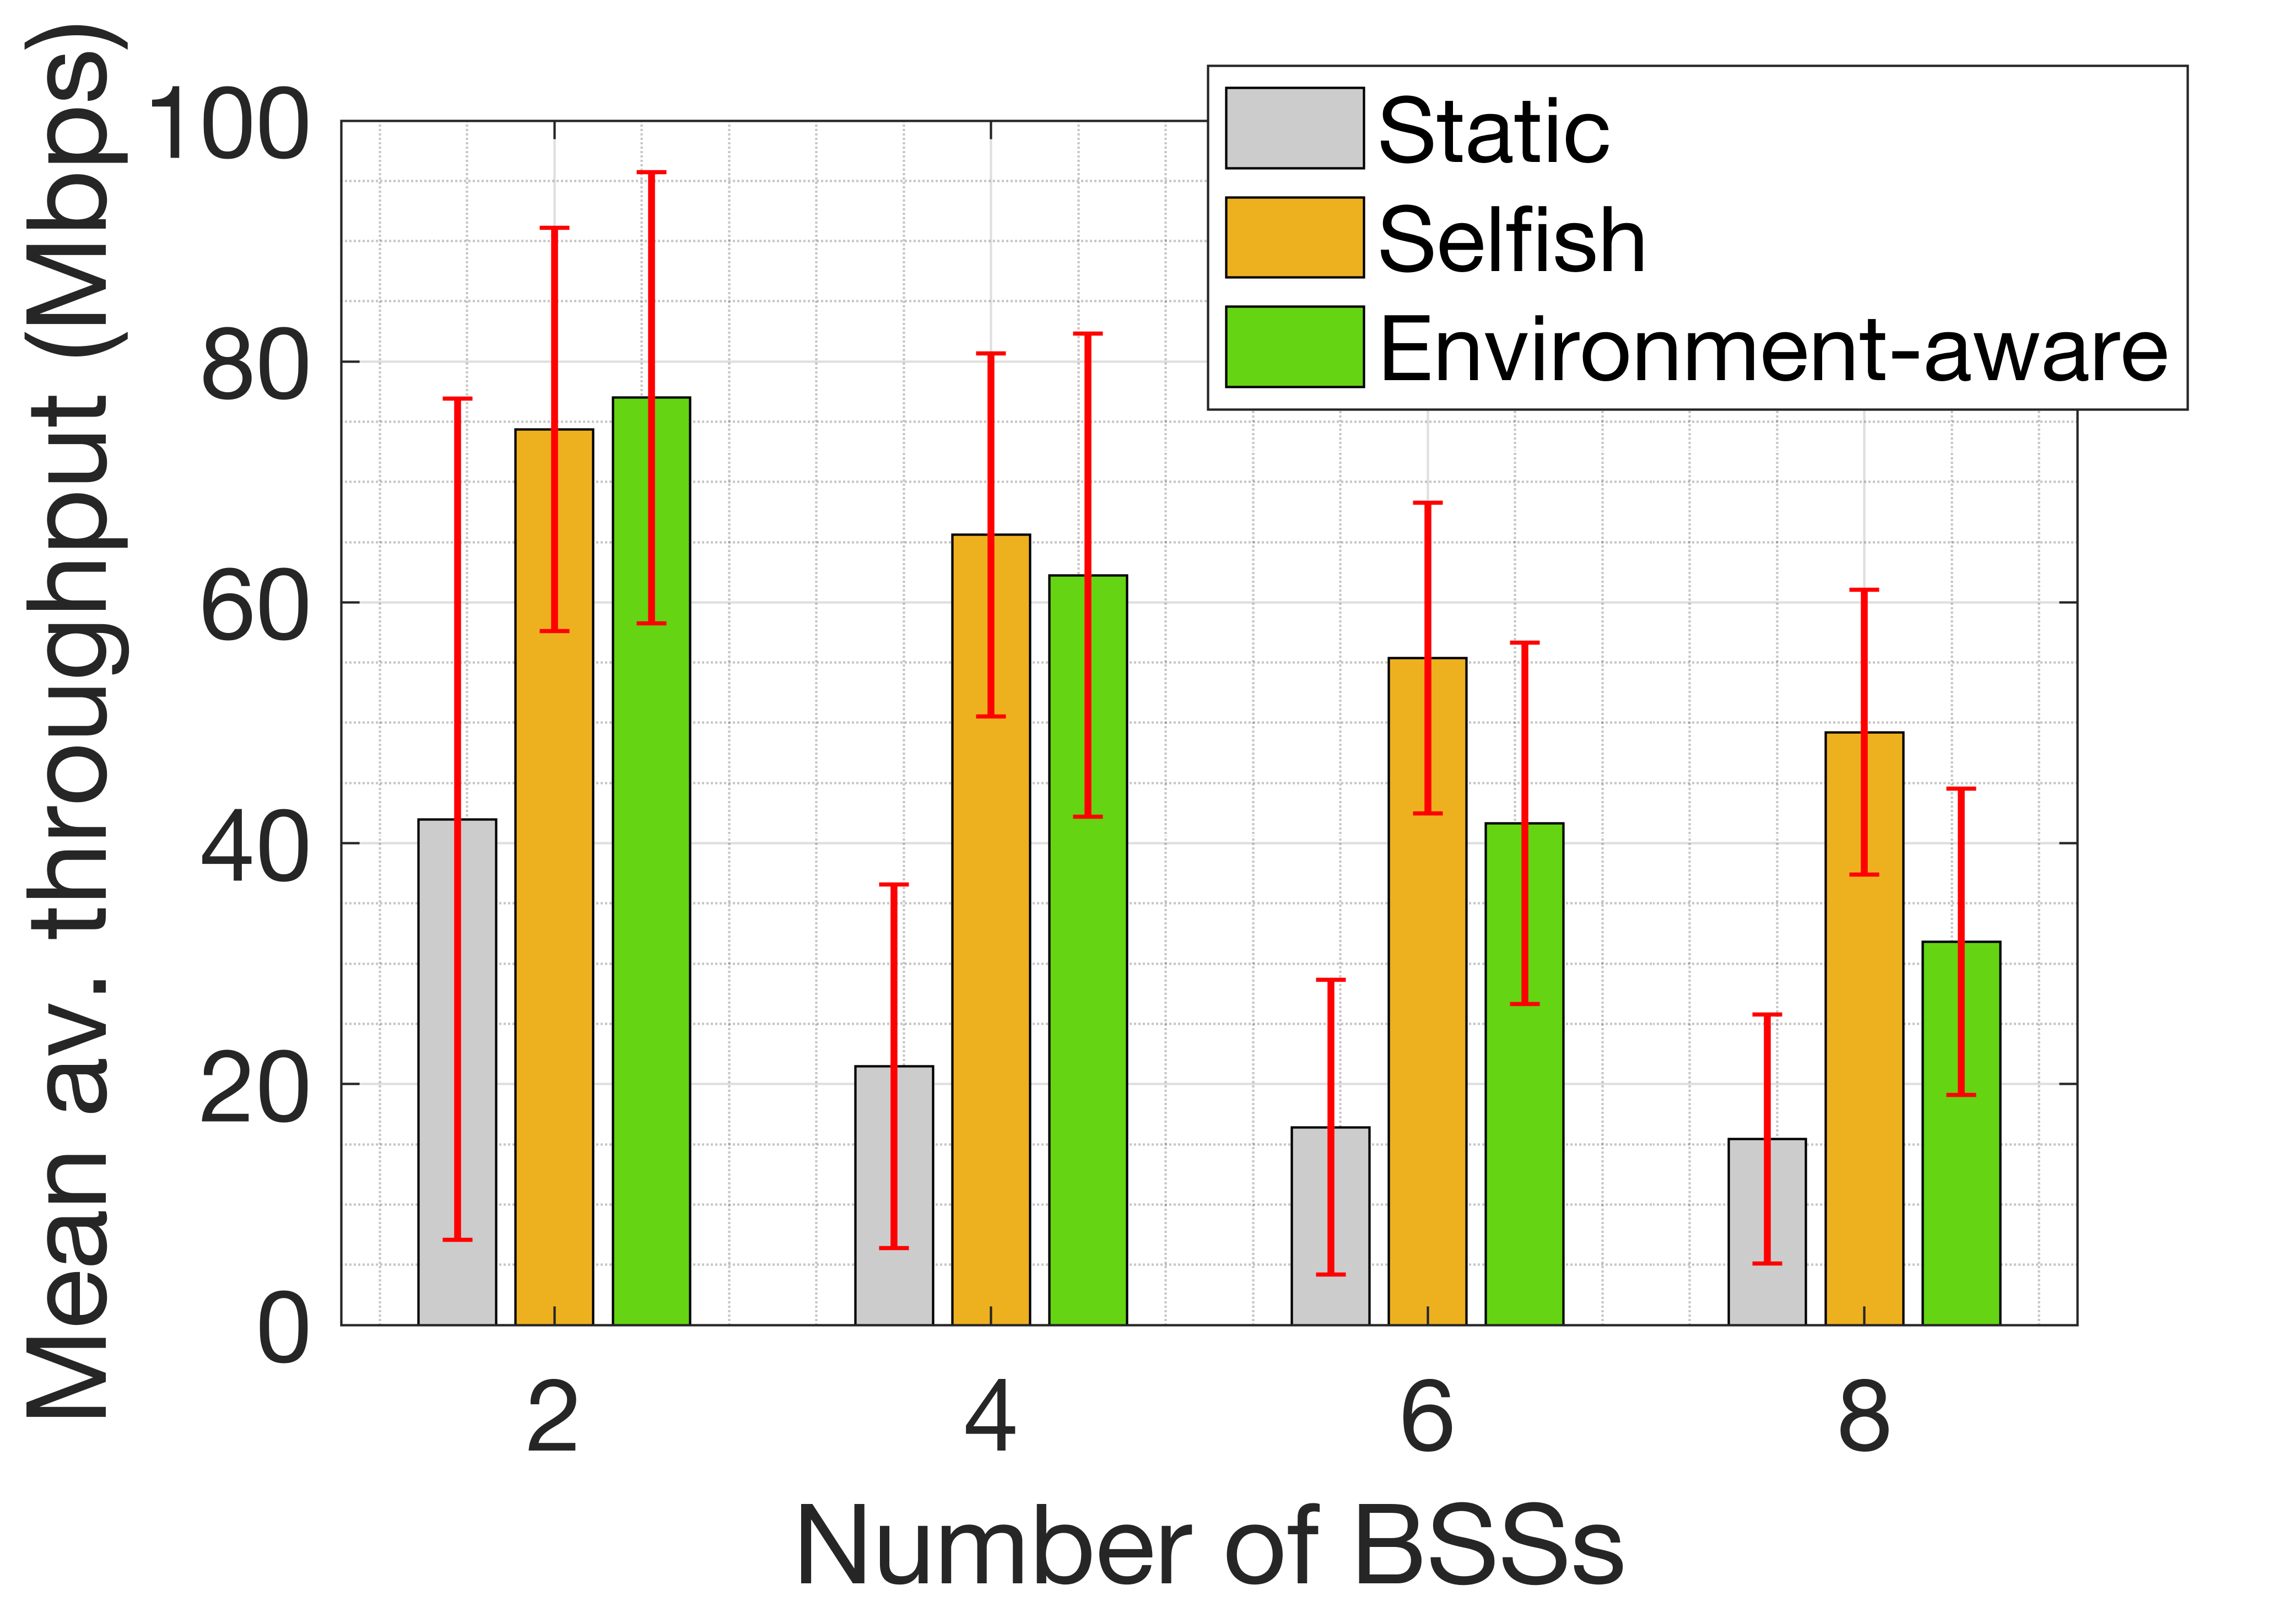
\includegraphics[width=0.4\textwidth]{images/paper_5_scalability_mean_tpt}}
	\subfigure[Max-min throughput]{\label{fig:paper_5_scalability_mean_maxmin}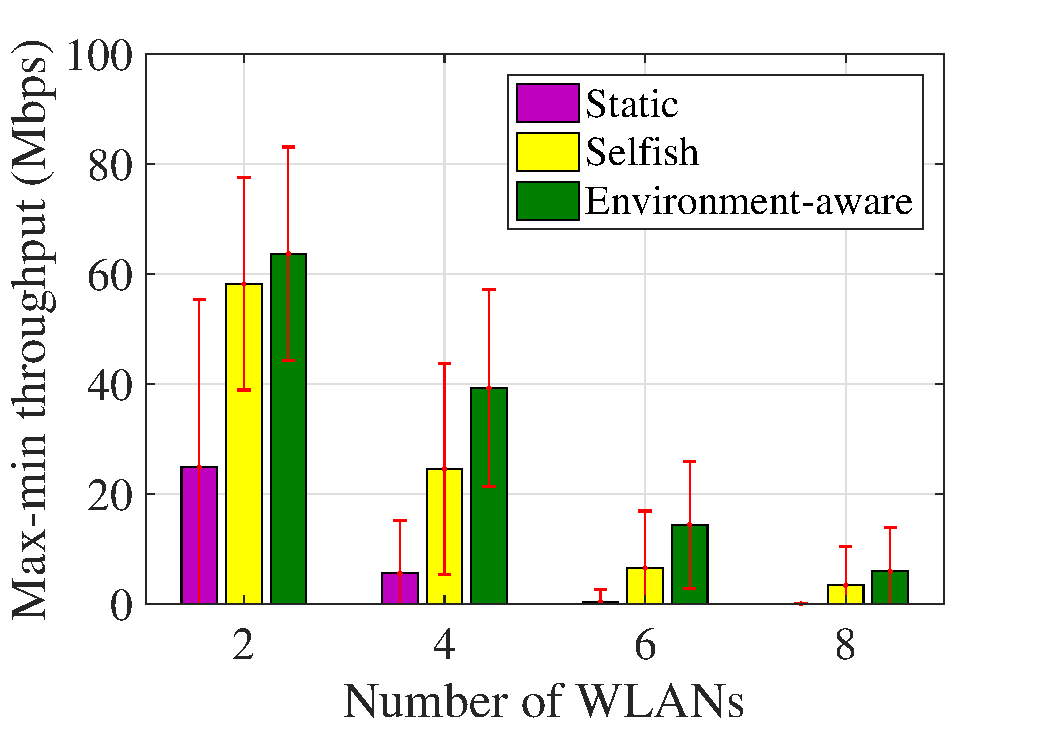
\includegraphics[width=0.4\textwidth]{images/paper_5_scalability_mean_maxmin}}
	\caption{Effect of cooperative vs non-cooperative rewards in a multi-player setting.}
	\label{fig:paper_5_scalability}
\end{figure*}

\begin{tcolorbox}
	\textbf{Finding \#6:} Bayesian-based exploration methods have the potential to address the non-stochasticity behind decentralized SR.
\end{tcolorbox} 

Regarding the learning procedure in decentralized SR (both selfish and collaborative settings), in \textbf{Paper \#2}, we showed that Bayesian-based exploration methods (e.g., Thompson sampling) perform well and grant better results than other types of algorithms that are indeed oriented to adversarial settings (e.g., EXP3). Notice that, as a result of the competition among multi-player SR agents, rewards distributions are highly non-stationary. Nevertheless, Bayesian exploration allows quick tracking of the best/worst performing actions but fails at identifying more subtle interactions when learning decentralized SR. This is illustrated in Figure \ref{fig:paper_4_bayesian_exploration}, which shows the temporal evolution of throughput obtained in an OBSS, for different exploration strategies. We considered the popular algorithms $\varepsilon$-greedy, EXP3, UCB, and Thompson sampling (TS). In the proposed setting, all the strategies allow finding the optimal global performance. Nevertheless, Thompson sampling does it more efficiently, thus reducing the variability on the throughput that results from exploration.

\begin{figure}[ht!]
	\centering
	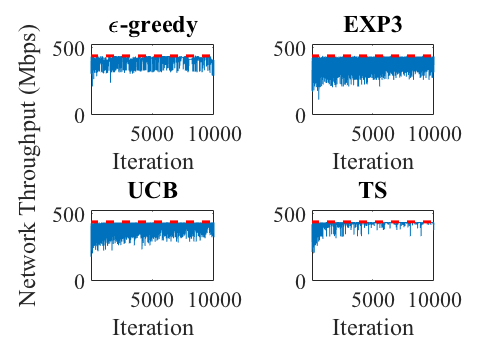
\includegraphics[width=.5\textwidth]{images/paper_4_bayesian_exploration}
	\caption{Temporal throughput achieved in an OBSS when applying different exploration methods in a multi-player setting.}
	\label{fig:paper_4_bayesian_exploration}
\end{figure}

\begin{tcolorbox}
	\textbf{Finding \#7:} Network dynamics and lack of information in local agents can severely affect the performance of sequential learning algorithms for decentralized SR.
\end{tcolorbox} 
In \textbf{Paper \#3}, we delved into practical aspects on the application of sequential learning to the decentralized SR problem (results are summarized in Figure \ref{fig:paper_5_considerations}):
\begin{enumerate}
	\item Networks are dynamic in different aspects (on/off devices, mobility, varying traffic requirements, channel fluctuations, etc.). This requires ML mechanisms to adapt to changes in the network, which entails the trade-off between old and new knowledge (how to assess data are becoming obsolete?). In this regard, we studied the effect of maintaining past information in sequential learning when significant changes in the network occur. In particular, we consider an OBSS whose topology changes radically at a given point (iteration 500). Figure \ref{fig:paper_5_change_network} shows the temporal evolution of the overall performance as a result of applying sequential learning. The fact is that multi-player MAB algorithms are shown to adapt to sudden changes in the network topology, which modify the global optimum completely. However, finding a joint configuration that improves the new situation's performance requires several training iterations, which may degrade network throughput if changes occur too fast.
	\item Sequential learning algorithms typically require rewards to be normalized. This normalization procedure is evident when the maximum achievable performance is known. However, this bound is unknown to the devices implementing SR and should, therefore, be approximated (e.g., by the maximum theoretical capacity, by the maximum data rate given the selected MCS, etc.). The fact of not knowing the upper bound reward of a given agent has implications on how learning is carried out (e.g., high variability, getting stuck in suboptimal actions, etc.). To study the effect of approximating the upper bound reward, we have considered a multi-agent setting composed of two BSSs. The temporal throughput of each BSS is shown in  Figure \ref{fig:paper_5_approx_vs_actual_tpt}, which compares the learning procedure that results from a known (in blue) and an approximated (in red) upper bound reward. As illustrated, the approximated metric leads to a higher throughput variability since agents cannot precisely differentiate optimal actions from others leading to lower performance.
	\item Sharing a reward in a collaborative setting can be challenging for the SR problem. The fact is that inter-agent interactions appear/disappear according to the sensitivity and the transmit power, which is a key impediment for agents to learn the hidden reward distributions of each action. Sharing the reward with the appropriate neighbors is therefore critical. To show the possible effects of not sharing the reward properly, we have considered a two BSS deployment. We compare long and short-range reward sharing approaches (i.e., the radius used to determine the set of agents that share a reward). Figure \ref{fig:paper_5_clustering_benefits} shows the temporal throughput evolution of the two BSSs for each of the reward sharing approach. In this case, the short-range approach is the best since it allows considering only the agents that are implied in the spatial interactions (in red). In turn, the long-range sharing approach (in blue) leads to suboptimal performance because the throughput of independent agents is considered for building a collaborative reward, hence introducing noise to the learning procedure.
\end{enumerate}

\begin{figure*}[ht!]
	\centering
	\subfigure[Network dynamics]{\label{fig:paper_5_change_network}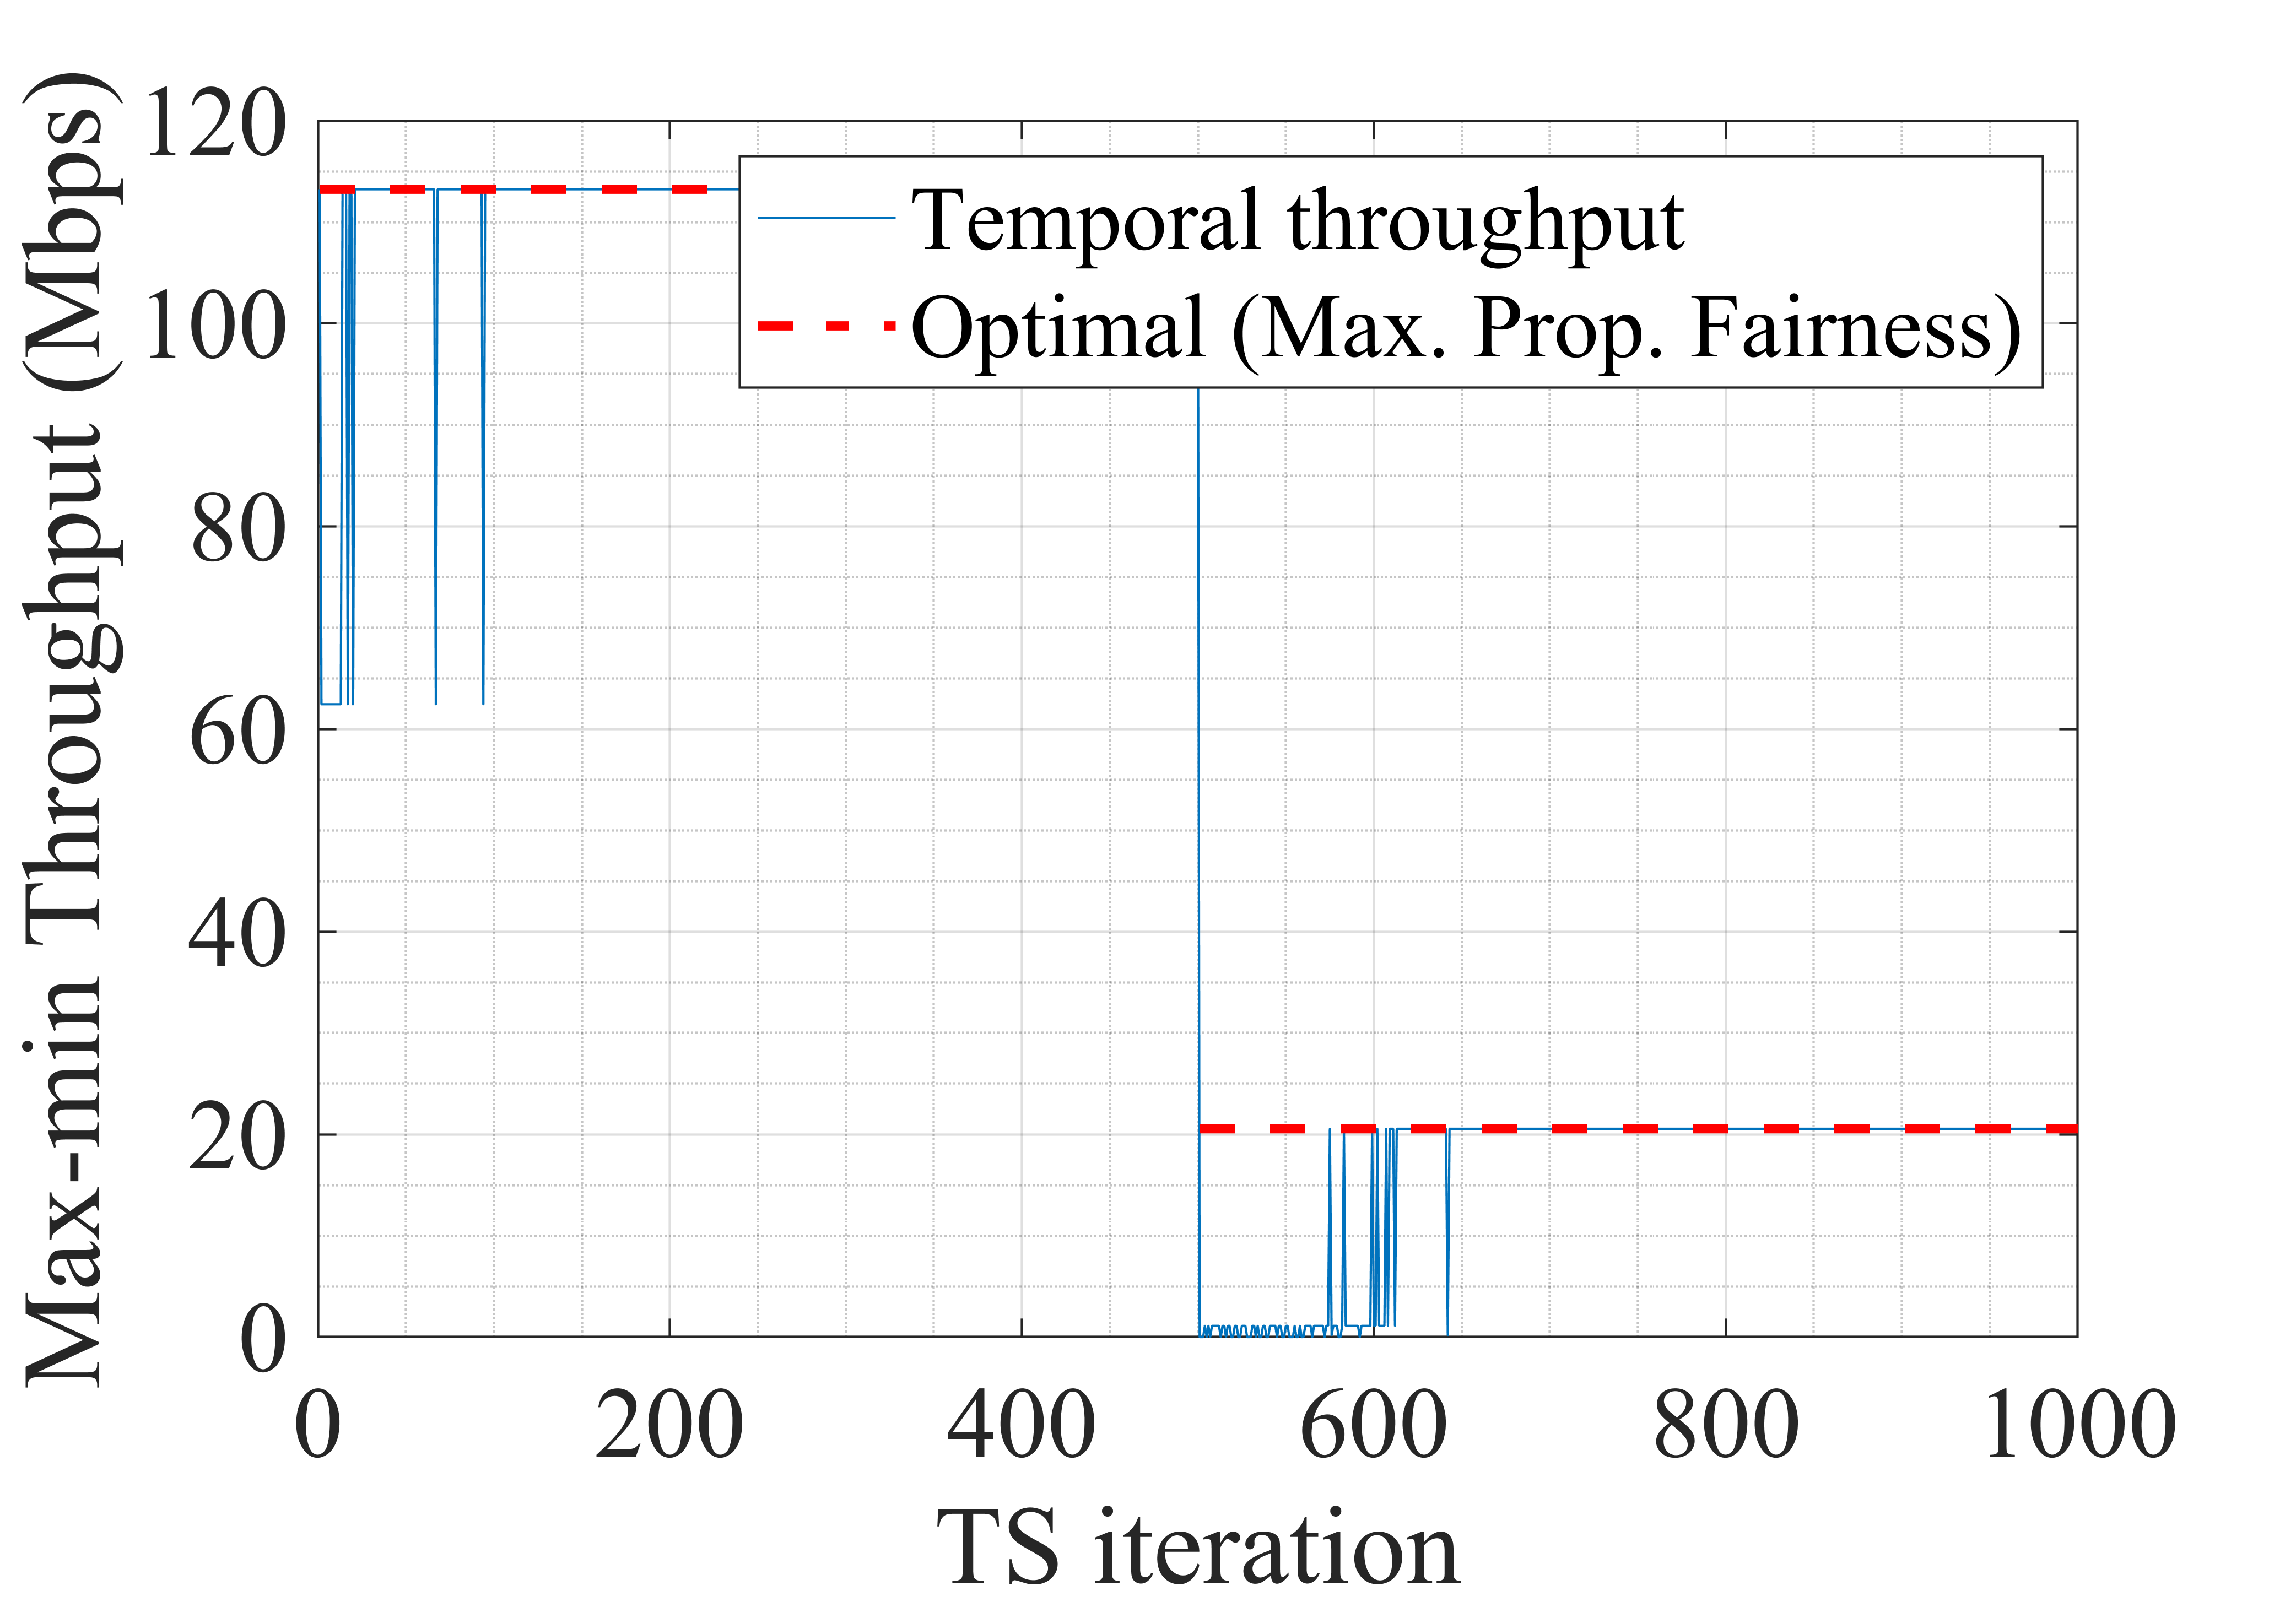
\includegraphics[width=0.32\textwidth]{images/paper_5_change_network}}
	\subfigure[Approximated upper bound]{\label{fig:paper_5_approx_vs_actual_tpt}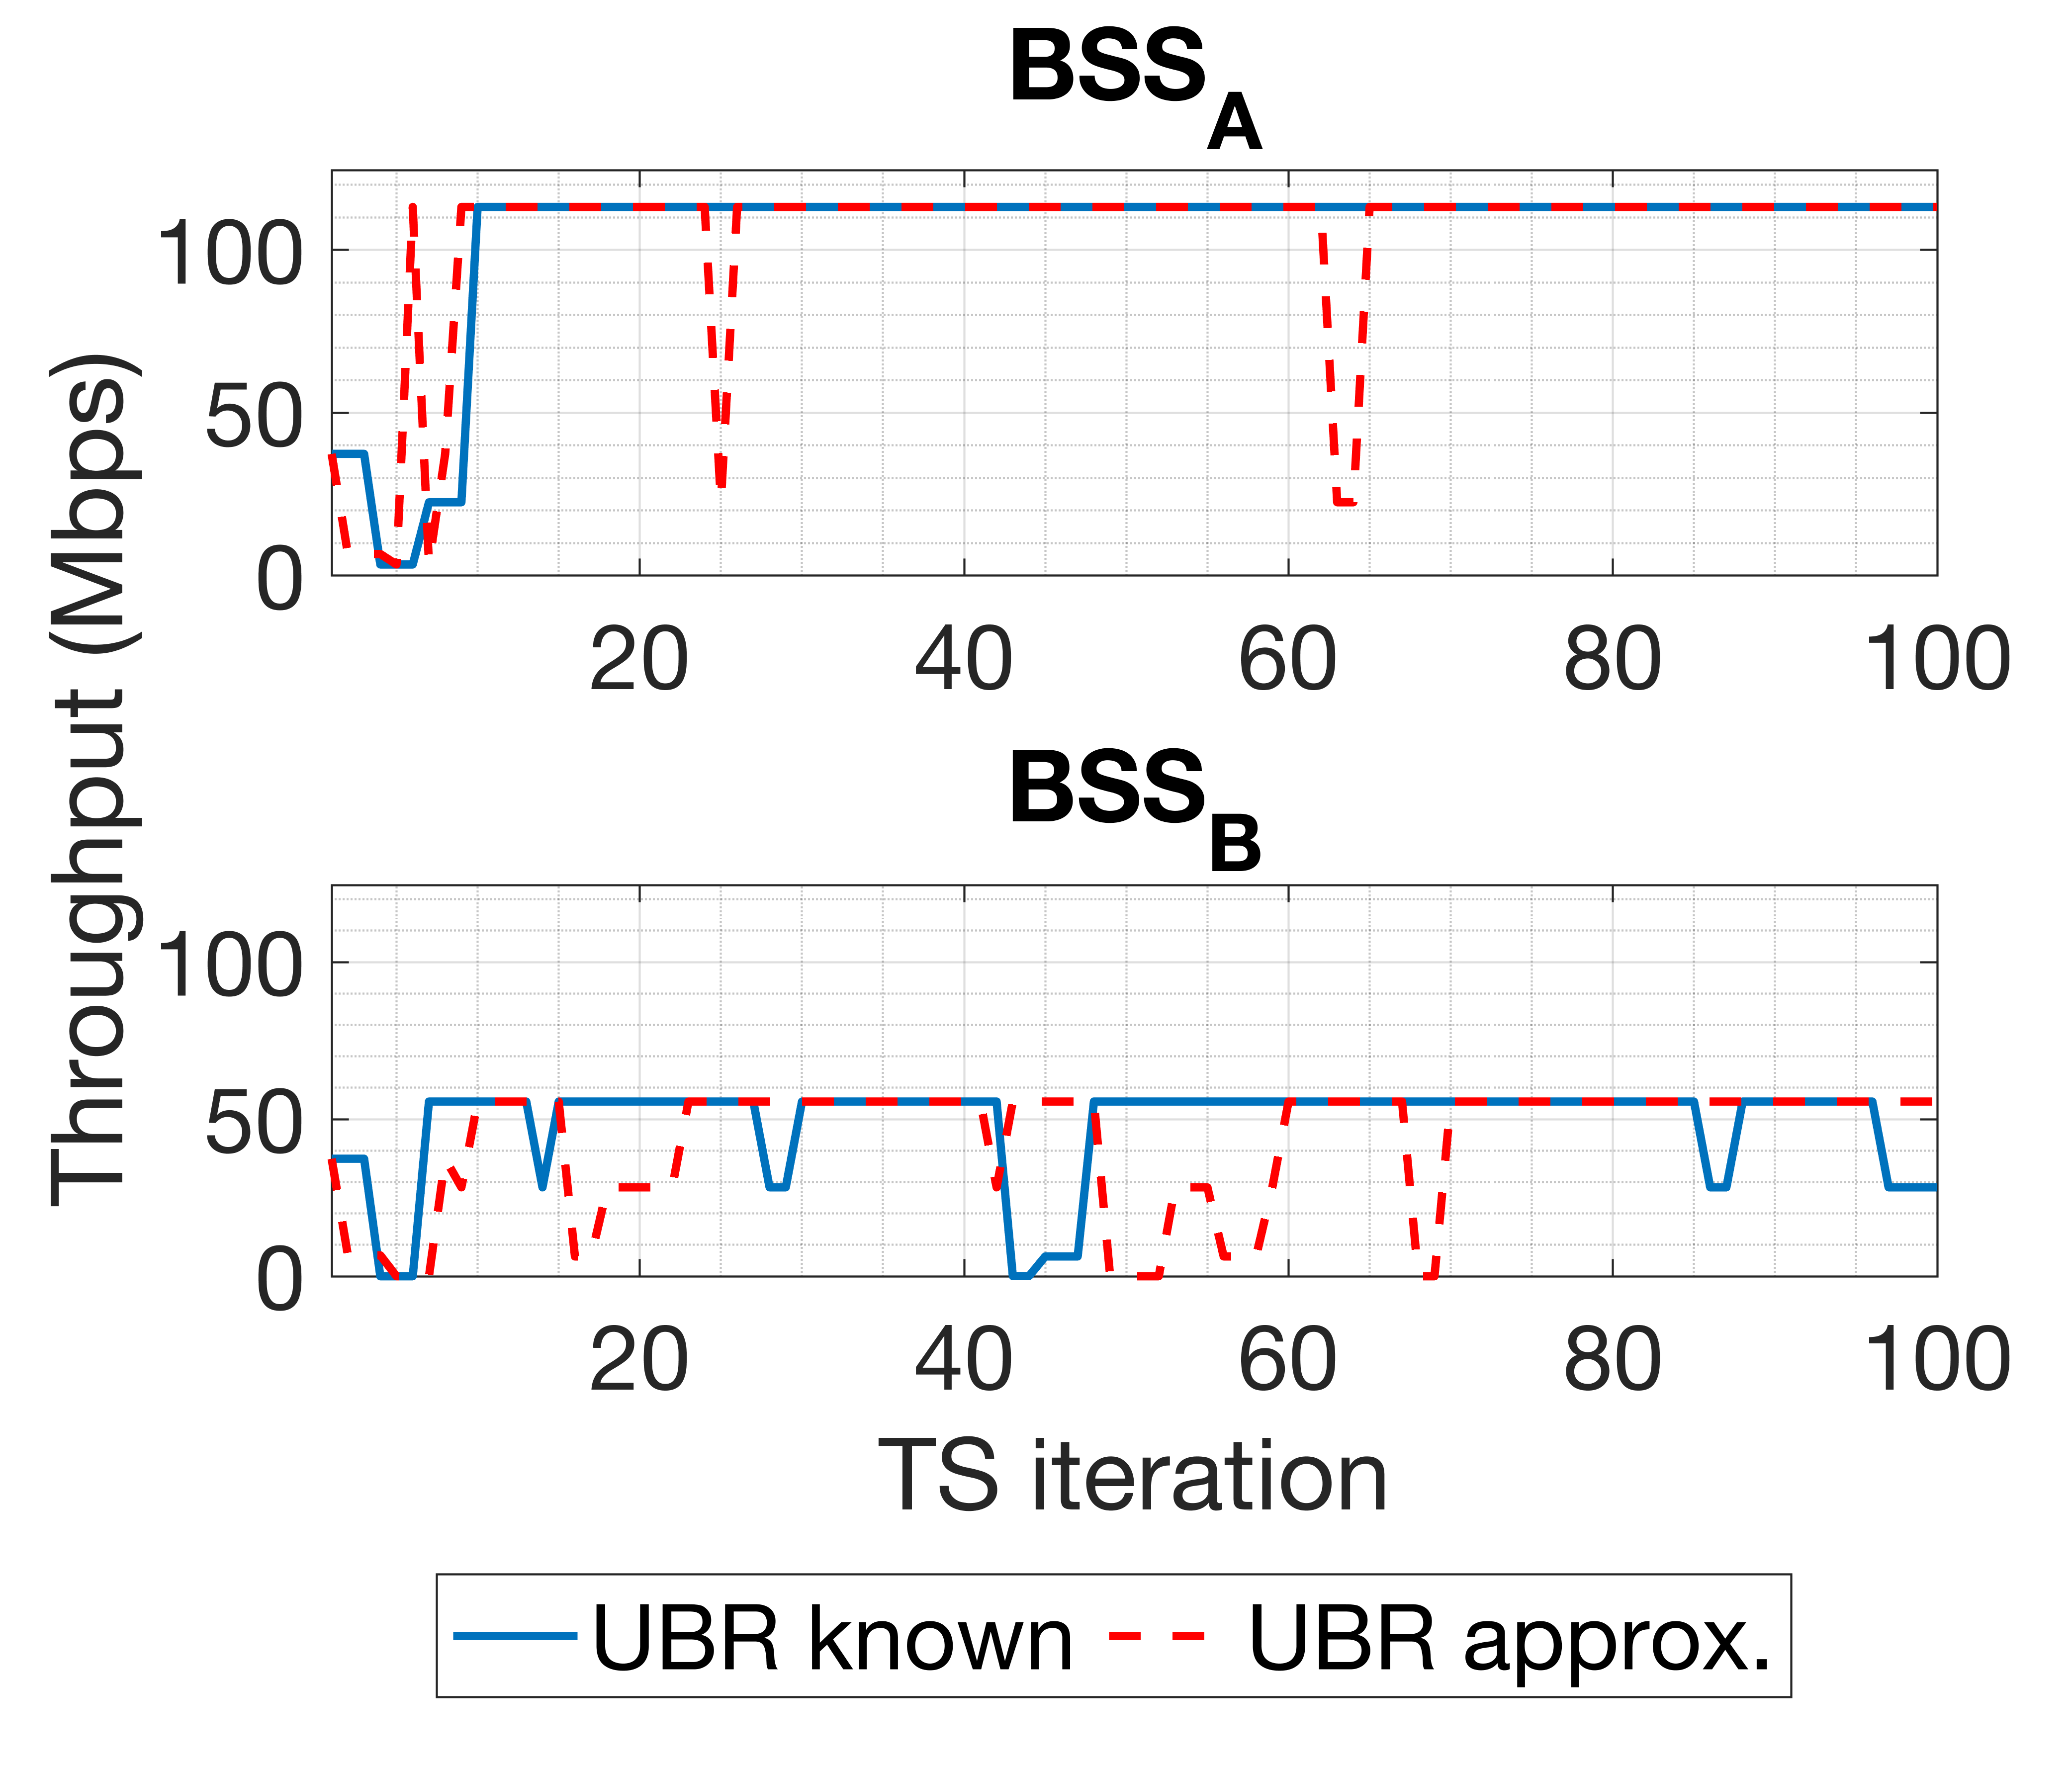
\includegraphics[width=0.33\textwidth]{images/paper_5_approx_vs_actual_tpt}}
	\subfigure[Collaboration considerations]{\label{fig:paper_5_clustering_benefits}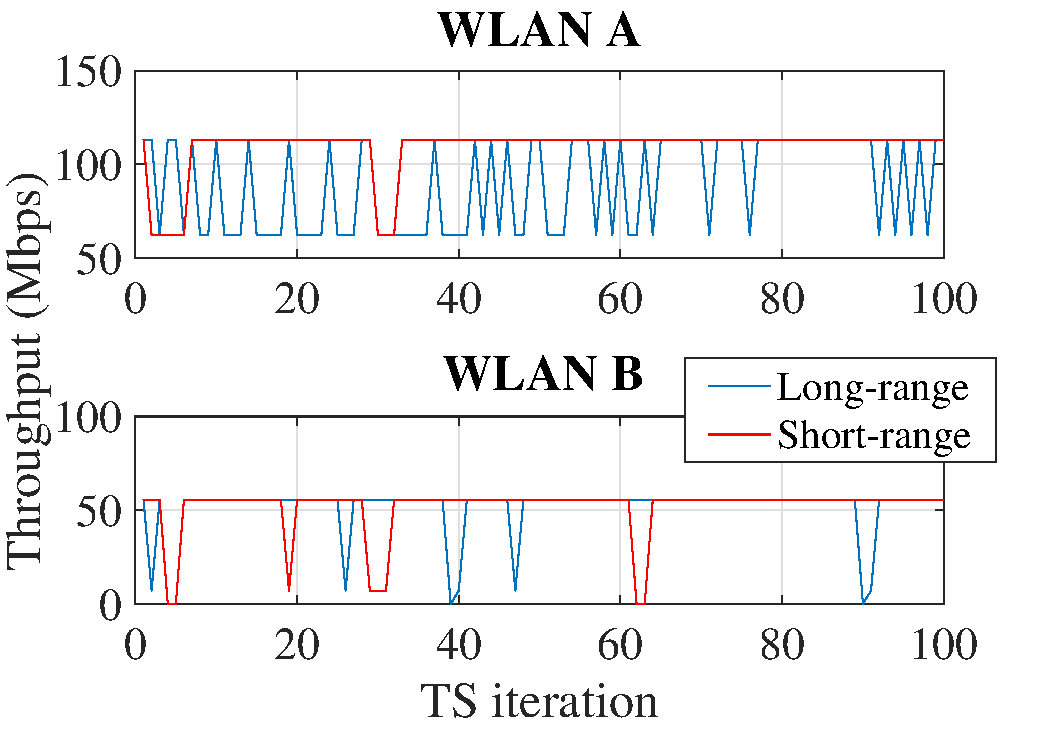
\includegraphics[width=0.33\textwidth]{images/paper_5_clustering_benefits}}
	\caption{Practical considerations for the application of sequential learning to decentralized Spatial Reuse.}
	\label{fig:paper_5_considerations}
\end{figure*}

%%%%%%%%%%%%%%%%%
% CONCLUSIONS
%%%%%%%%%%%%%%%%%
\chapter{Concluding Remarks}
\label{chapter6}

% Work done
In this thesis, we investigated the viability of addressing SR in future IEEE 802.11 WLANs from a decentralized perspective. To that purpose, we first provided an in-depth study of the current 11ax SR operation and analyzed its ways forward through the 11be amendment. Then, we proposed the use of ML for addressing the uncertainty and non-stochasticity resulting from the concurrent adaptation of sensitivity and transmit power by devices in an OBSS. This approach entails a set of challenges related to multi-player agent settings, which are also studied in this thesis. In particular, the competition among nodes leads to a game-theoretic setting, where notions on equilibriums gain significance. In this regard, we showed the main challenges that WLANs may face when applying sequential learning mechanisms for SR, including efficiency and convergence aspects. In order to conduct our research, we analytically modeled the SR operation and analyzed the new kind of interactions among BSSs. Besides, we implemented the 11ax SR operation in an ML-enabling network simulator, which allowed us to study the performance gains of SR and the proposed solutions based on sequential learning.

% Main findings
Our main findings confirm the potential of SR for improving dense wireless networks' capacity, especially on enhancing the average delay in an OBSS. Apart from that, we have shown that the decentralized SR mechanisms proposed in this thesis improve the default carrier sense approach and to enhance the performance in enterprise and residential-like scenarios effectively. However, the application of ML in a multi-player setting leads to a set of implications that may severely affect the fairness and the global performance of an OBSS. We based part of our research on analyzing the effects of selfish and collaborative methods for multi-agent SR.

% Future work
We left as future work the potential of coordinated and centralized mechanisms to further enhance SR in next-generation WLANs. In this regard, an interesting topic lies in the trade-off between the potential achievable improvements and the corresponding overhead, which may include data acquisition, data exchange, or synchronization. Future research work also encompasses the convergence of SR with other technologies such as beamforming/null steering \cite{psr2019}, OFDMA \cite{bankov2018ofdma, dovelos2018optimal}, multiple antenna systems \cite{liao2016mu}, or scheduled transmissions \cite{nurchis2019target}, and whether their joint operation can improve separate optimization. In this regard, AI may contribute to addressing the inherent complexity of end-to-end communications systems, thus revealing the potential of moving beyond block-based optimization. Finally, regarding the multi-agent setting, important research questions remain open concerning convergence aspects or training under dynamic topologies.

%% AI 
%Finally, AI emerges as a potential solution to address SR because of the complexity of the problem and the characteristics of dense WLAN deployments, which are typically decentralized and highly varying in terms of users and channel dynamics. Through AI, it is possible to capture and exploit complex information that cannot be predicted on before-hand (traffic demands, user behavior, varying interference regimes, etc.). As a result, a learning-based procedure can be conducted to further improve the performance of WLAN deployments. More insights on this are provided in Chapter \ref{chapter3}.

%%%%%%%%%%%%%%%%%
% BIBLIOGRAPHY
%%%%%%%%%%%%%%%%%
\bibliography{bibliography}

%%%%%%%%%%%%%%%%%%
%% ATTACHED PUBLICATIONS
%%%%%%%%%%%%%%%%%%
%\chapter{Publications}
%\label{chapter7}

\newpage

%\subfile{papers/paper1/Implications of Decentralized Q-Learning Resource Allocation in Wireless Networks.tex}

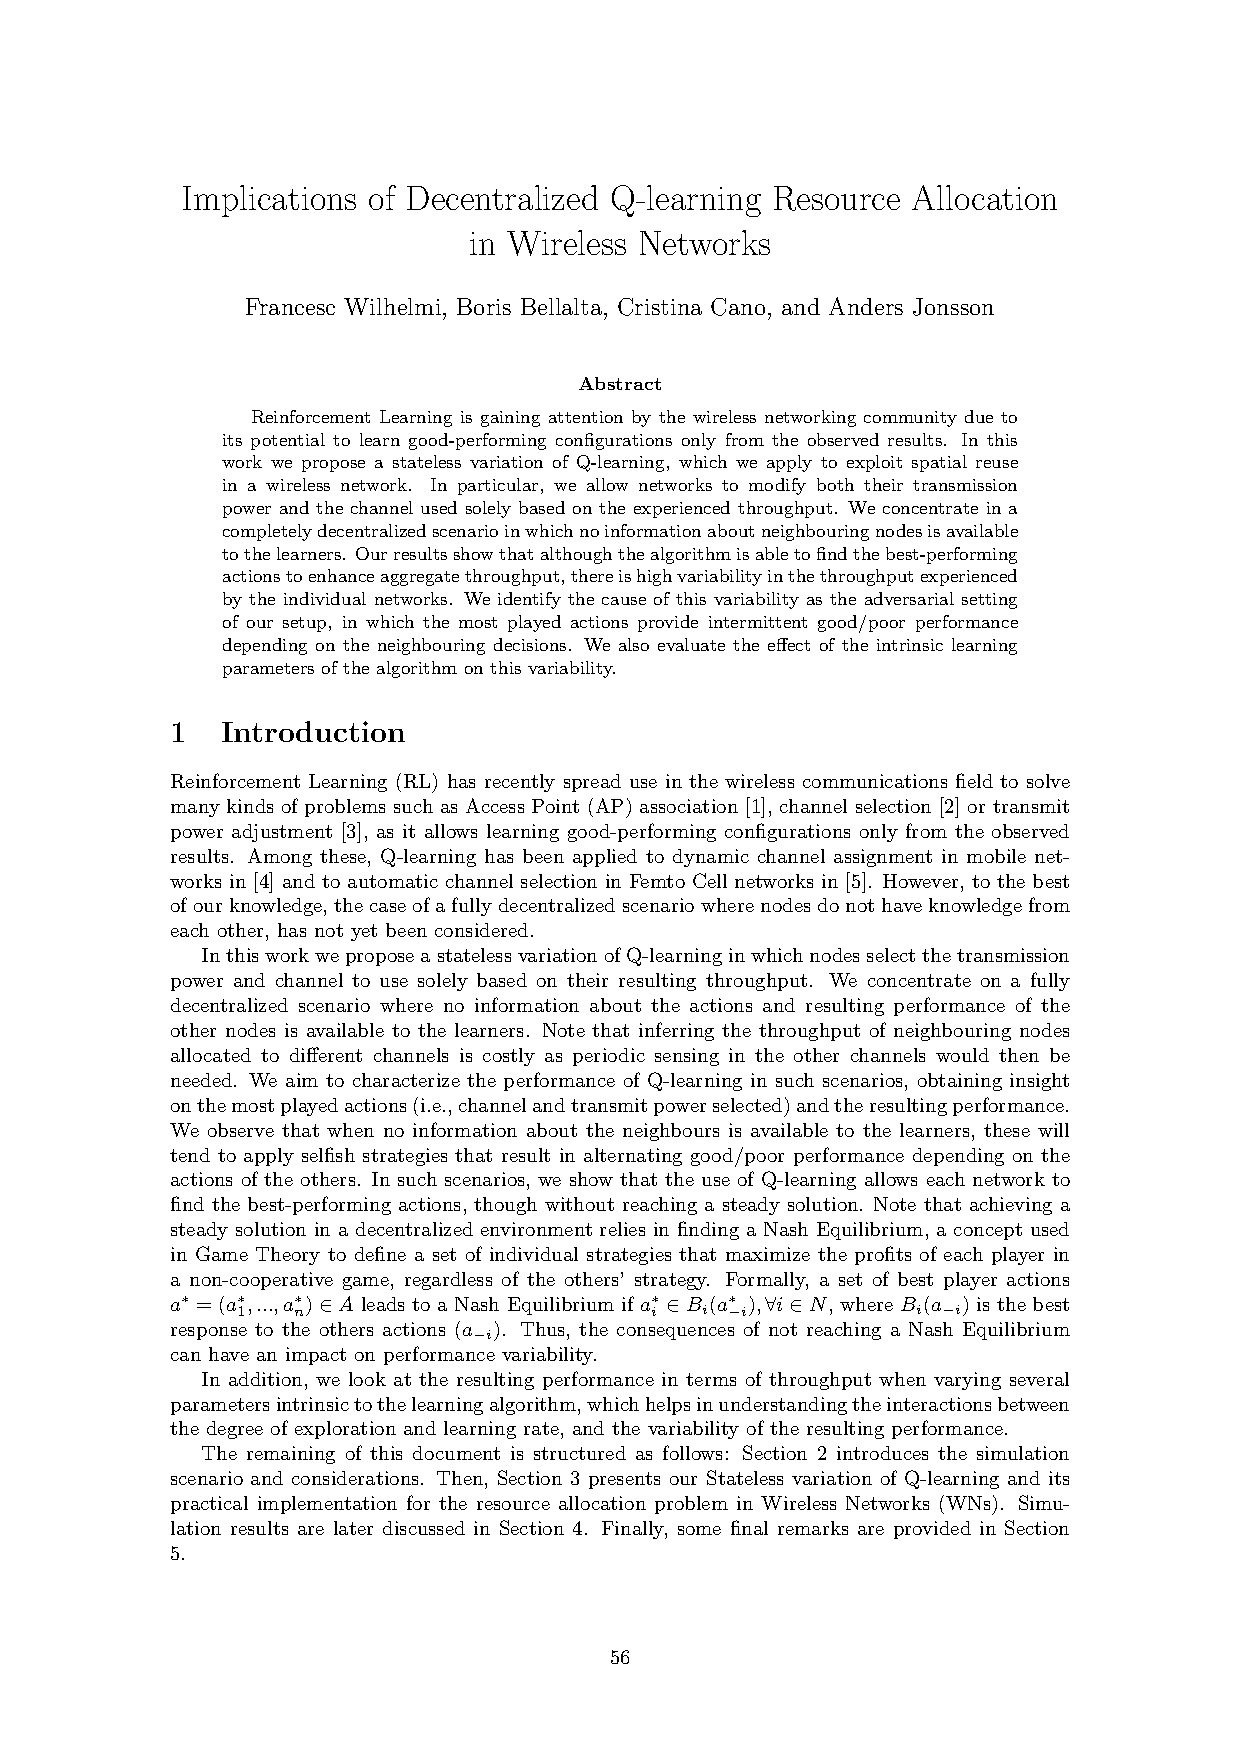
\includepdf[pages=1-]{papers/paper1/paper1.pdf}
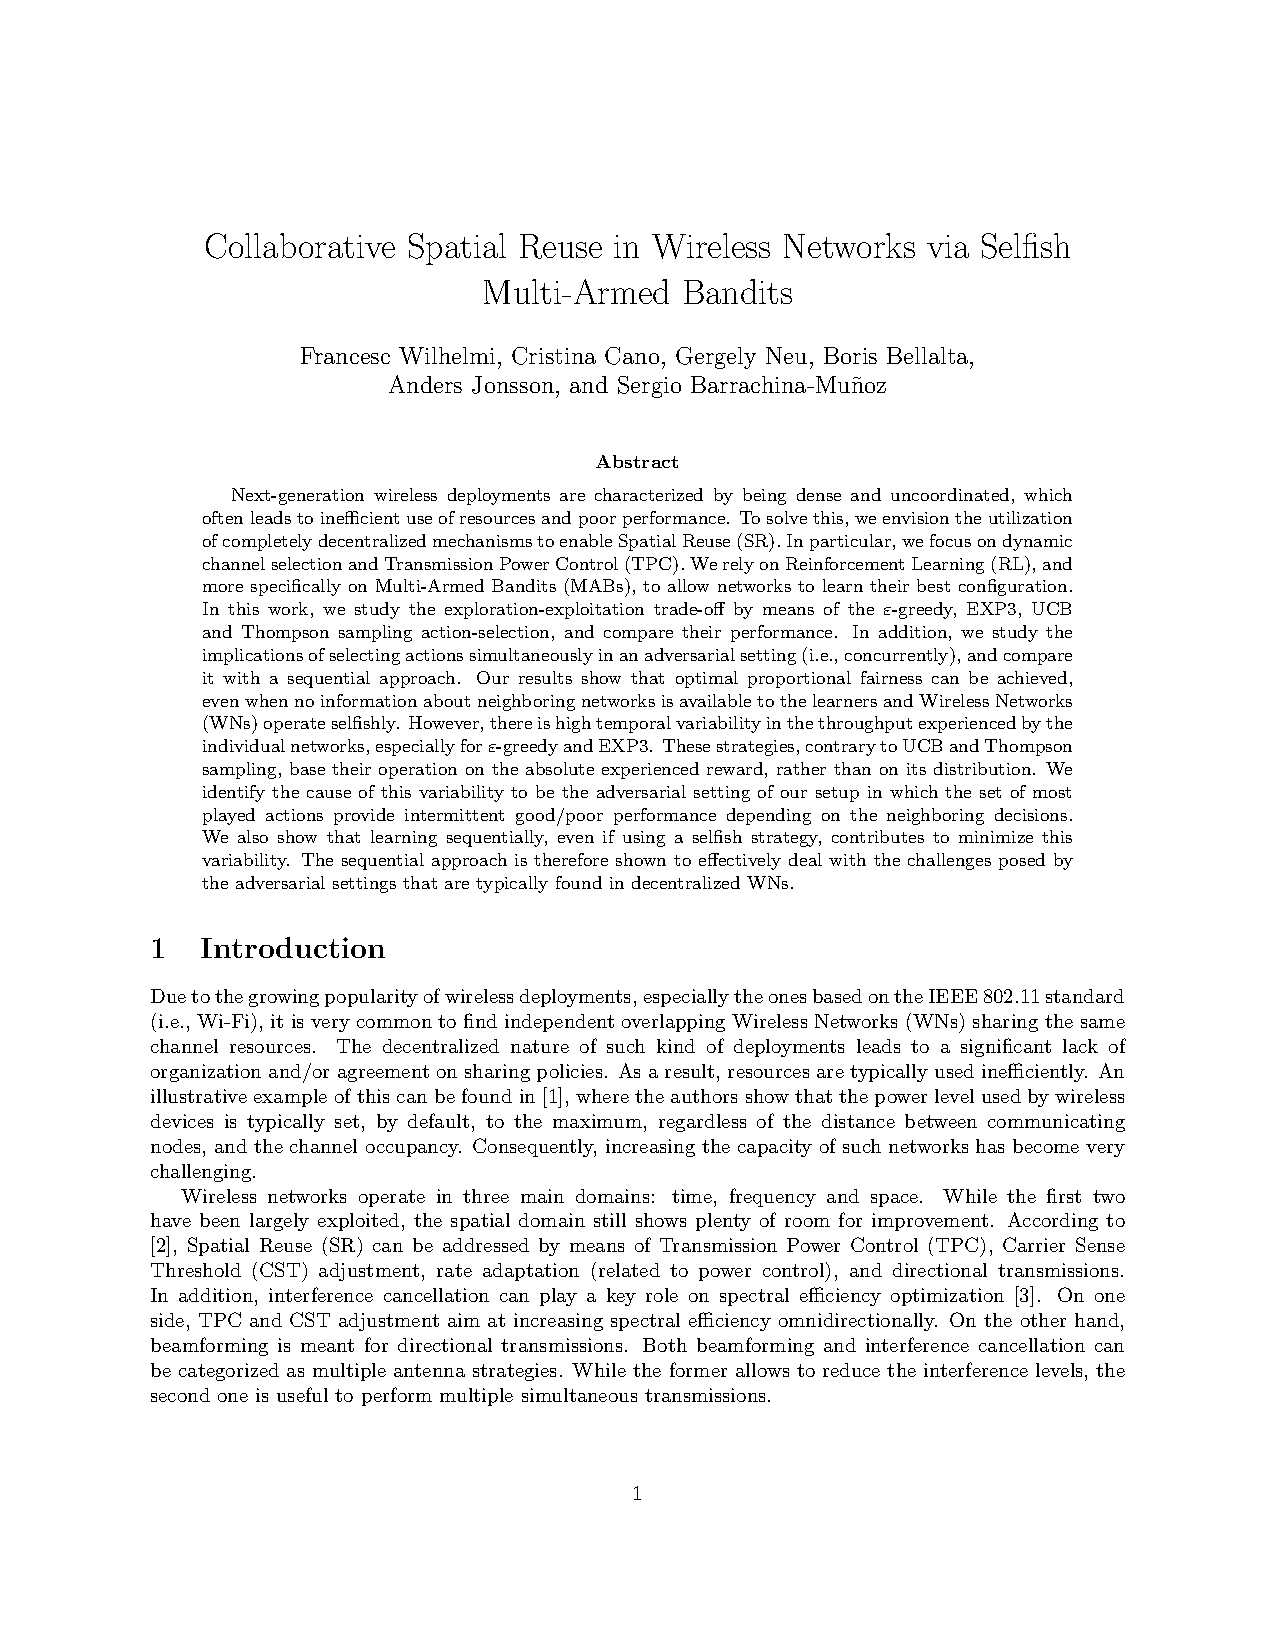
\includepdf[pages=1-]{papers/paper2/paper2.pdf}
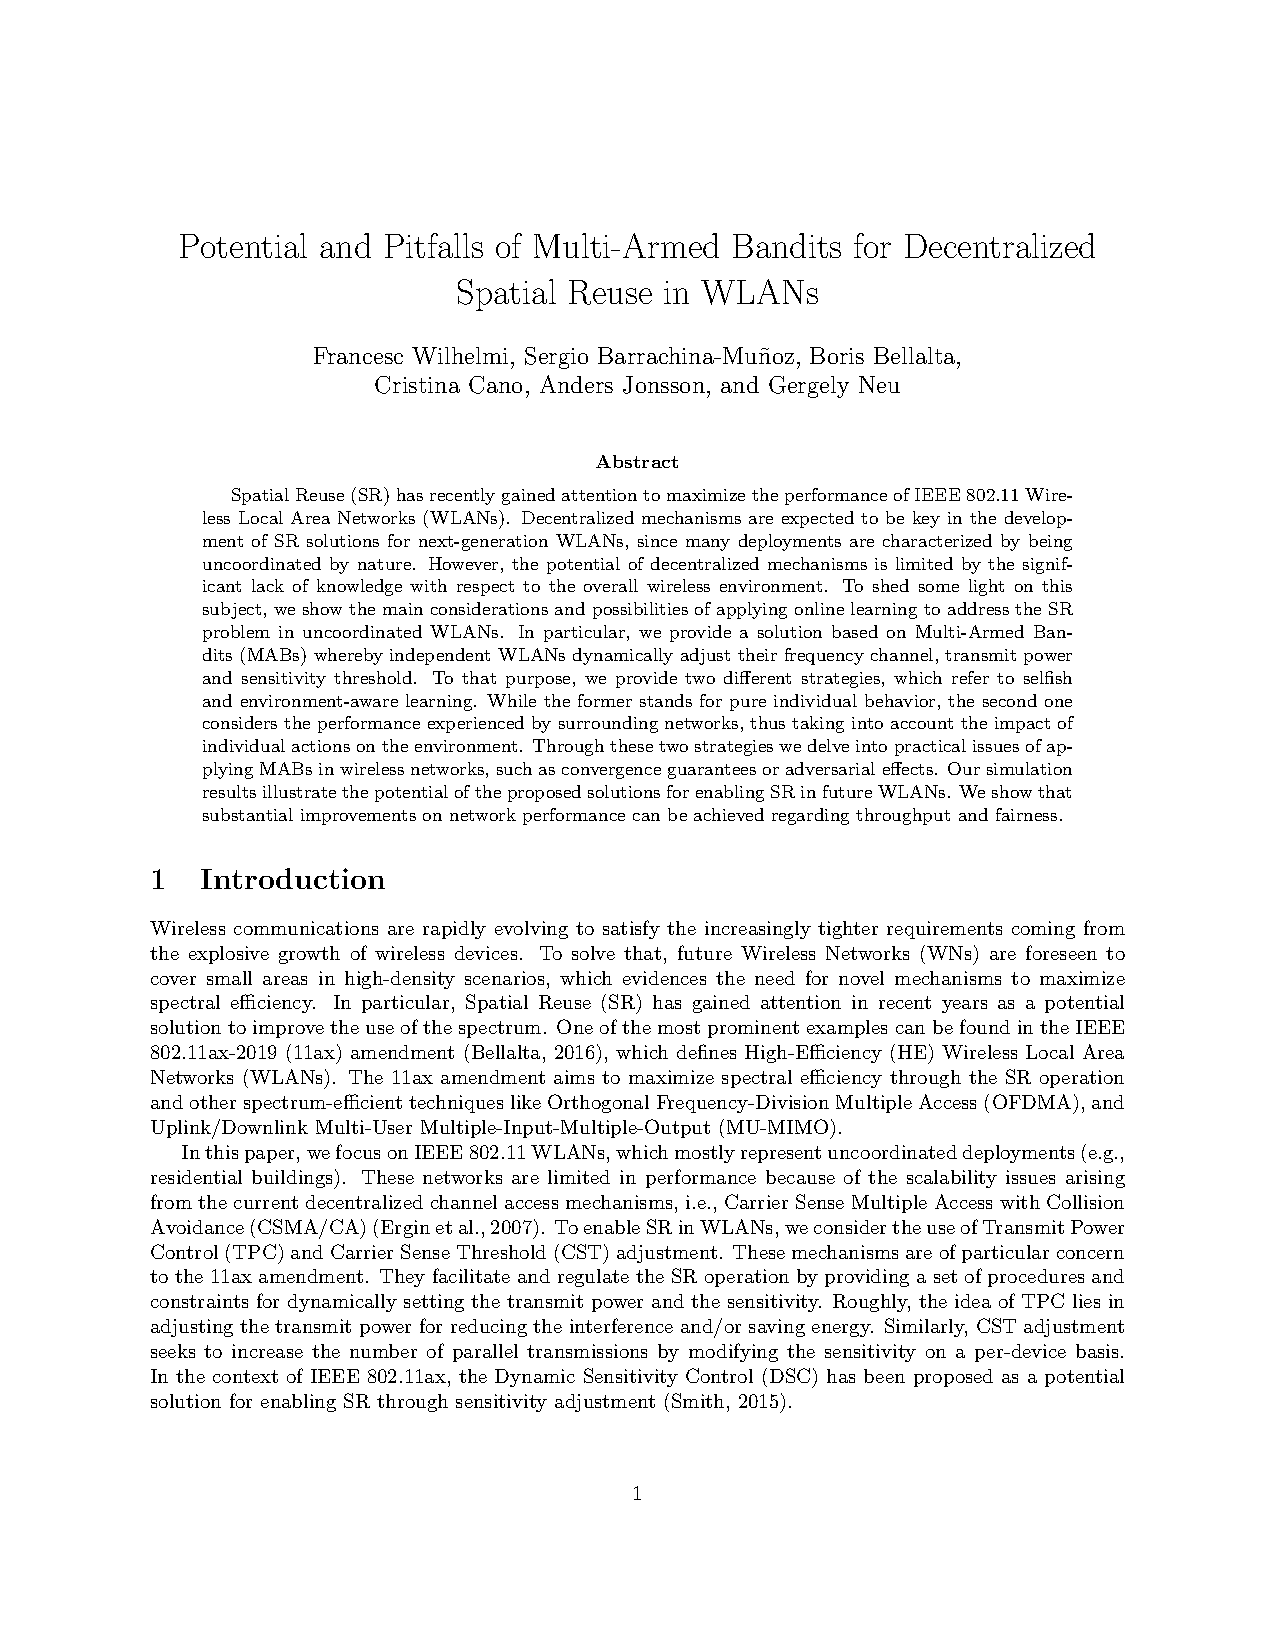
\includepdf[pages=1-]{papers/paper3/paper3.pdf}
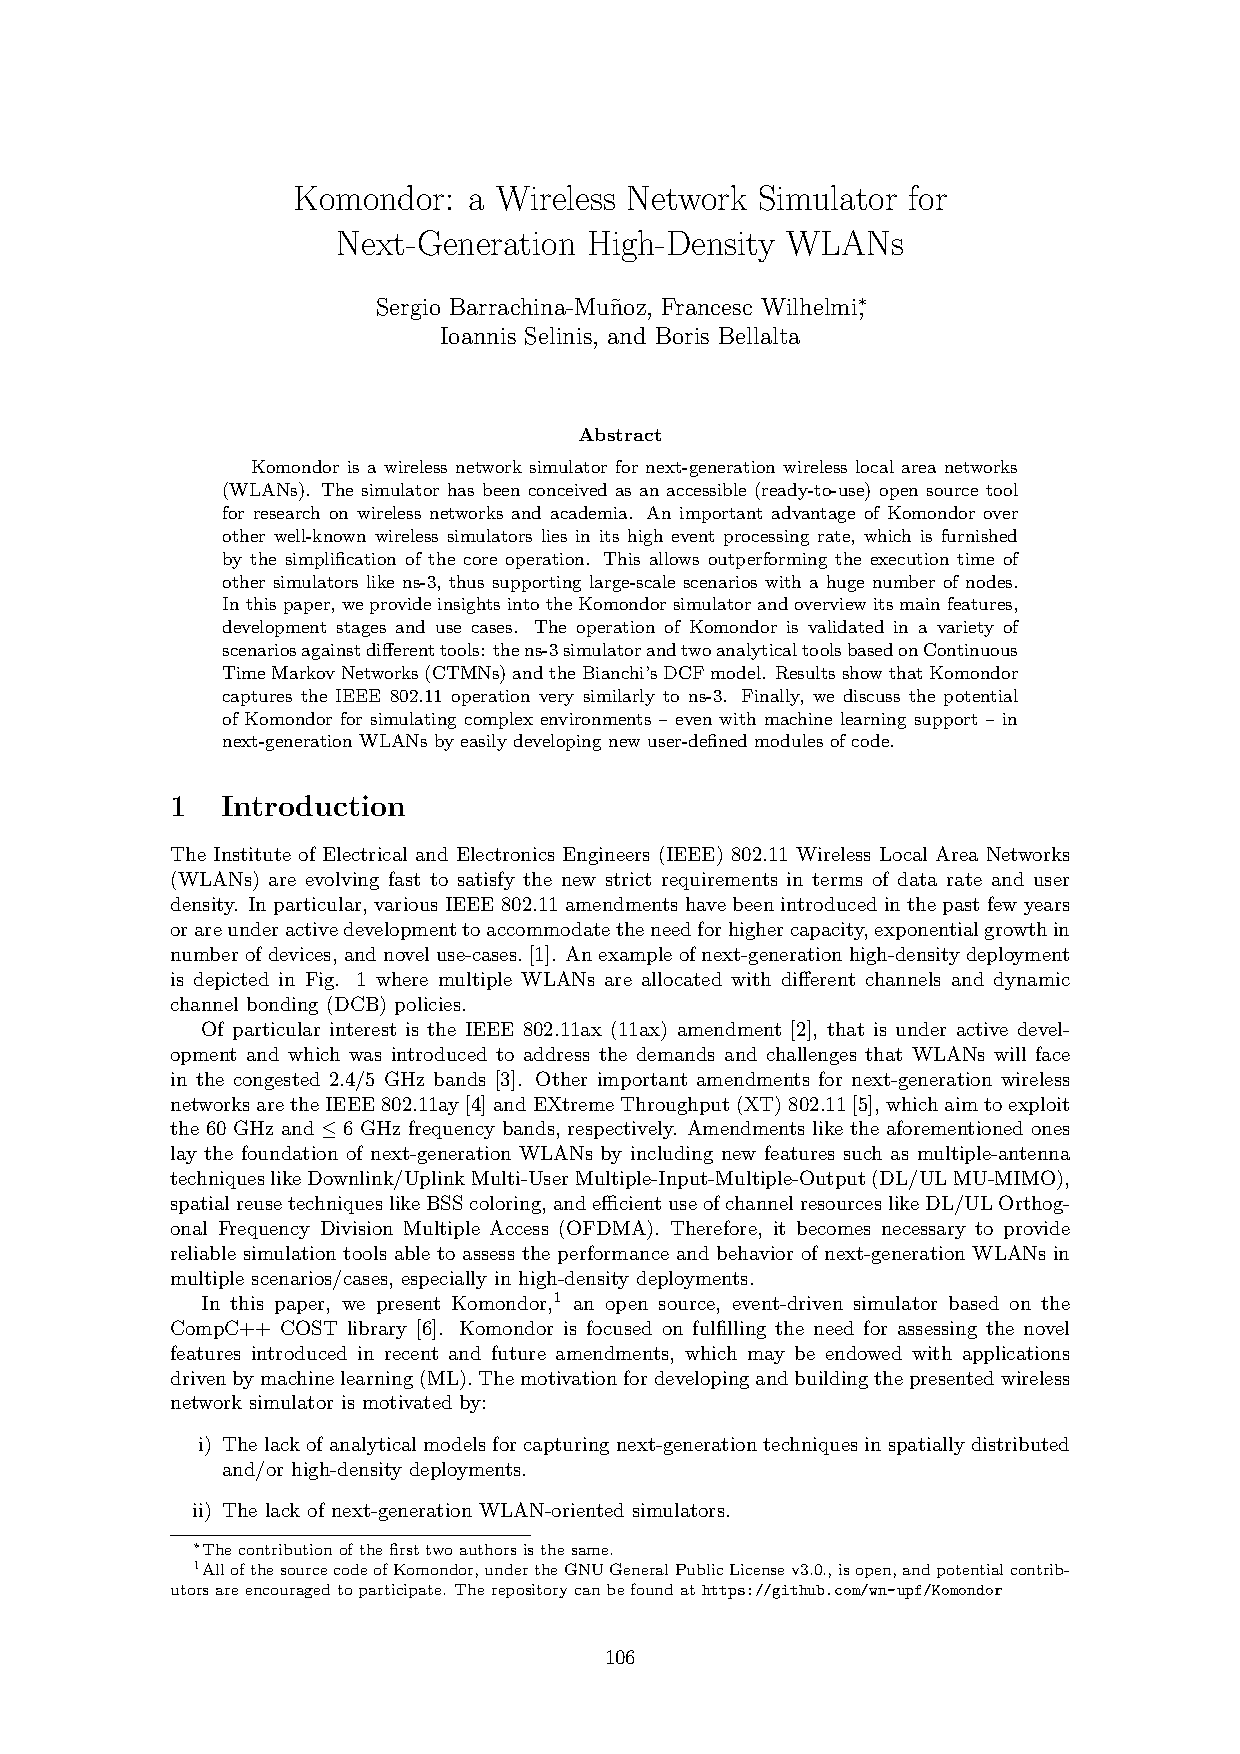
\includepdf[pages=1-]{papers/paper4/paper4.pdf}
\includepdf[pages=1-]{papers/paper5/paper5.pdf}
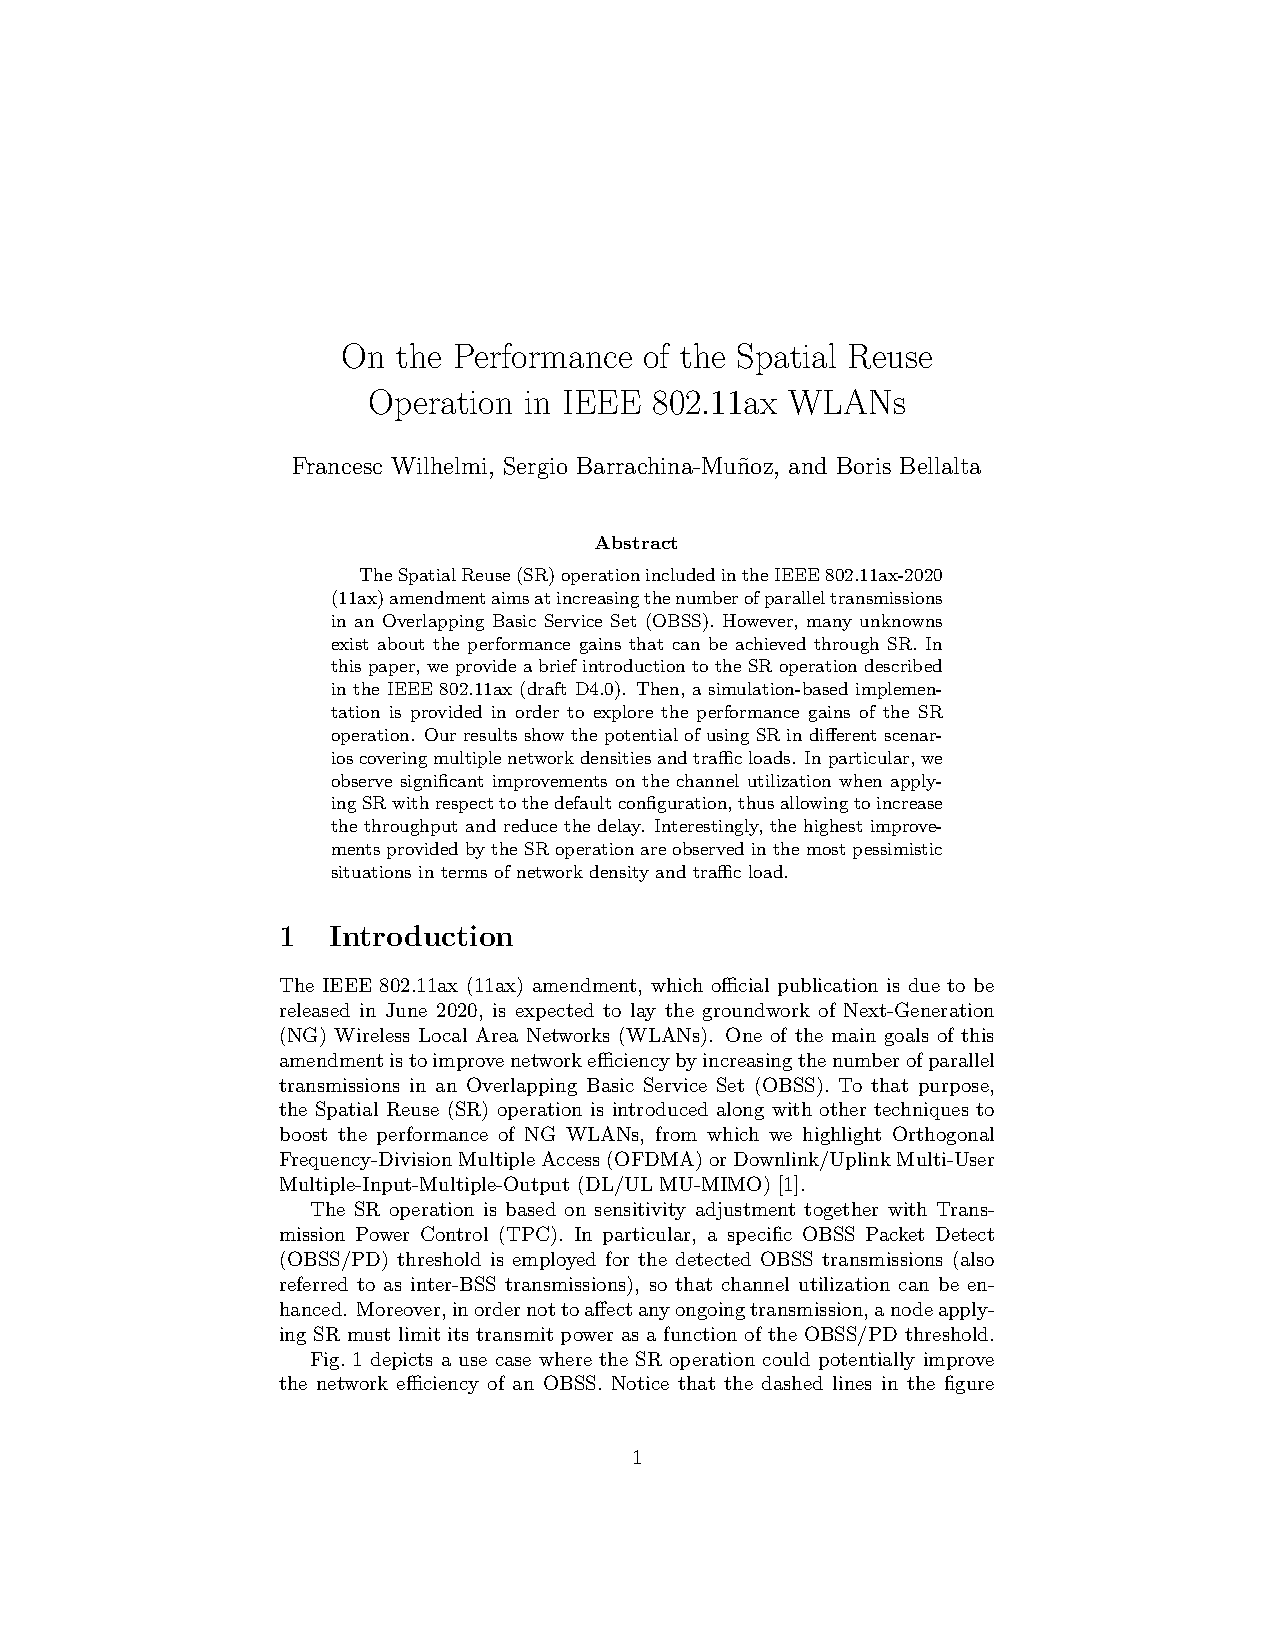
\includepdf[pages=1-]{papers/paper6/paper6.pdf}
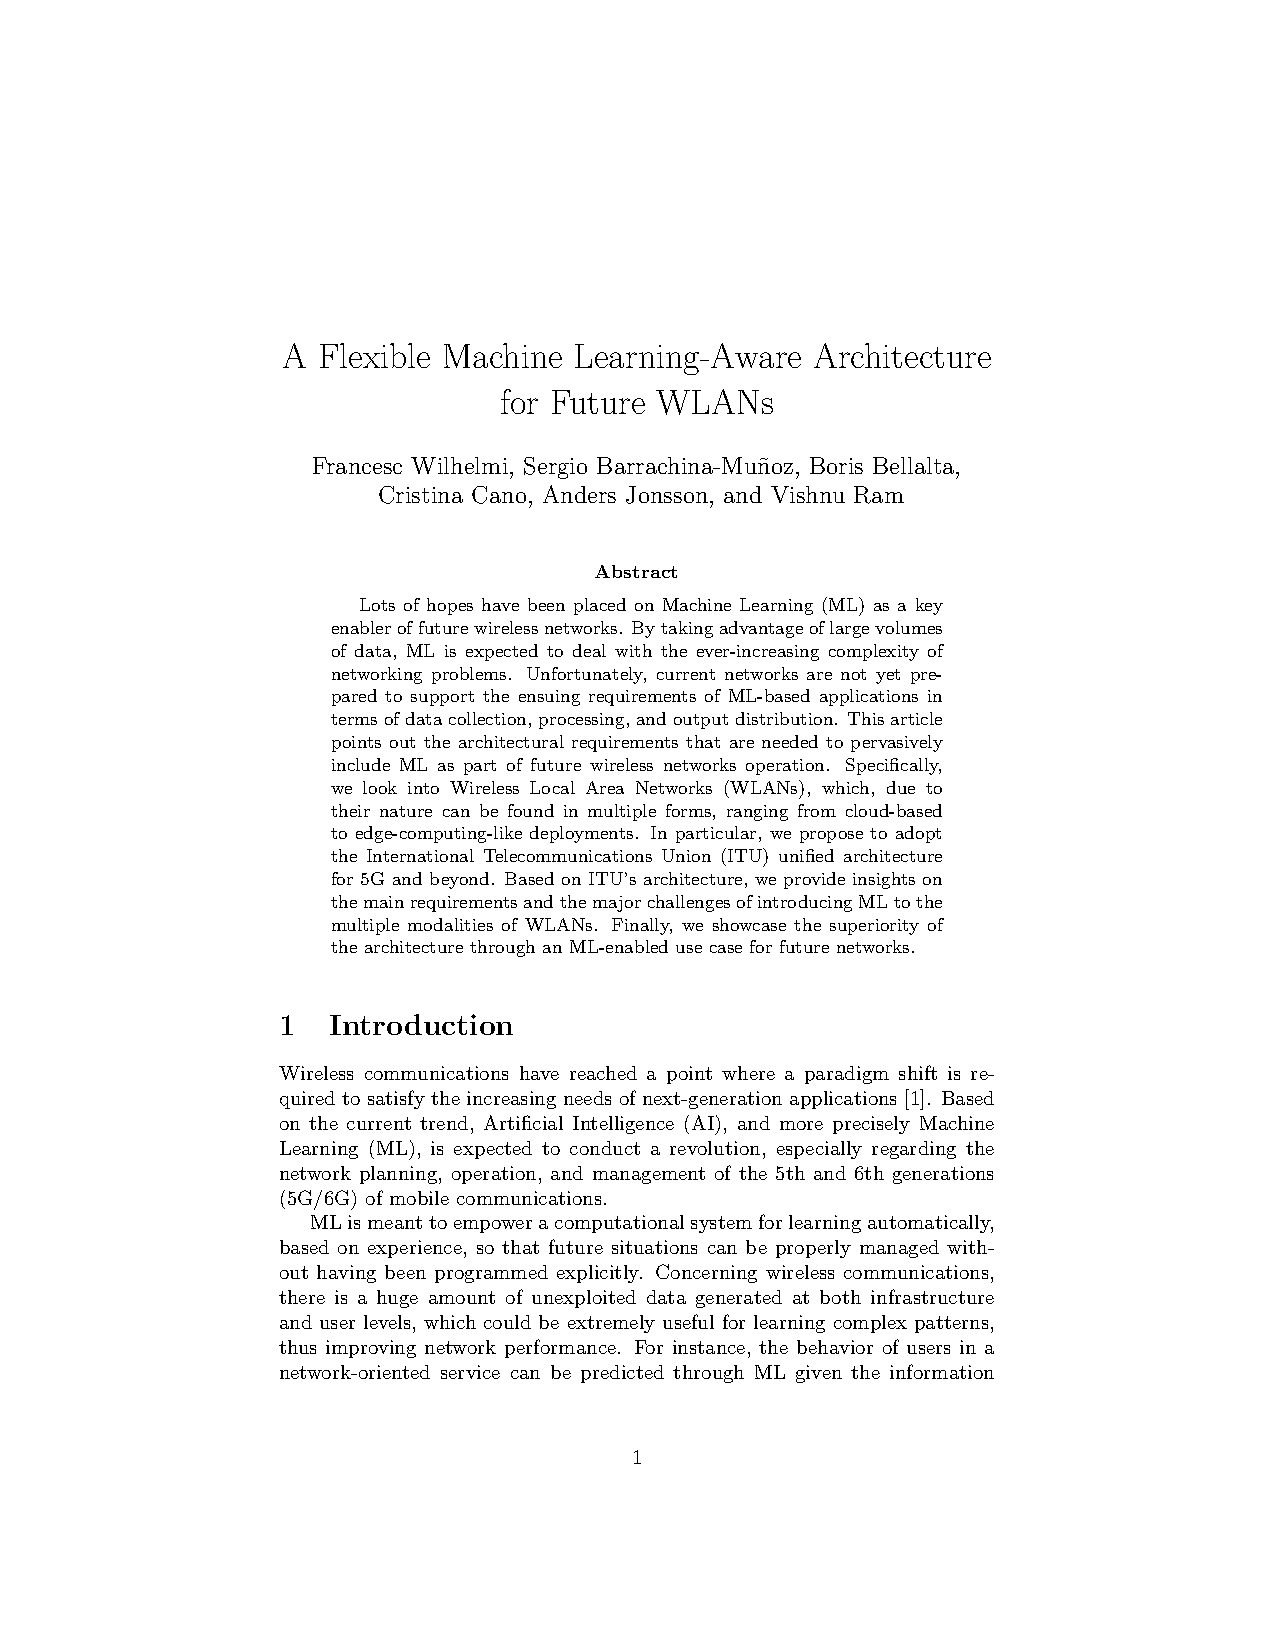
\includepdf[pages=1-]{papers/paper7/paper7.pdf}
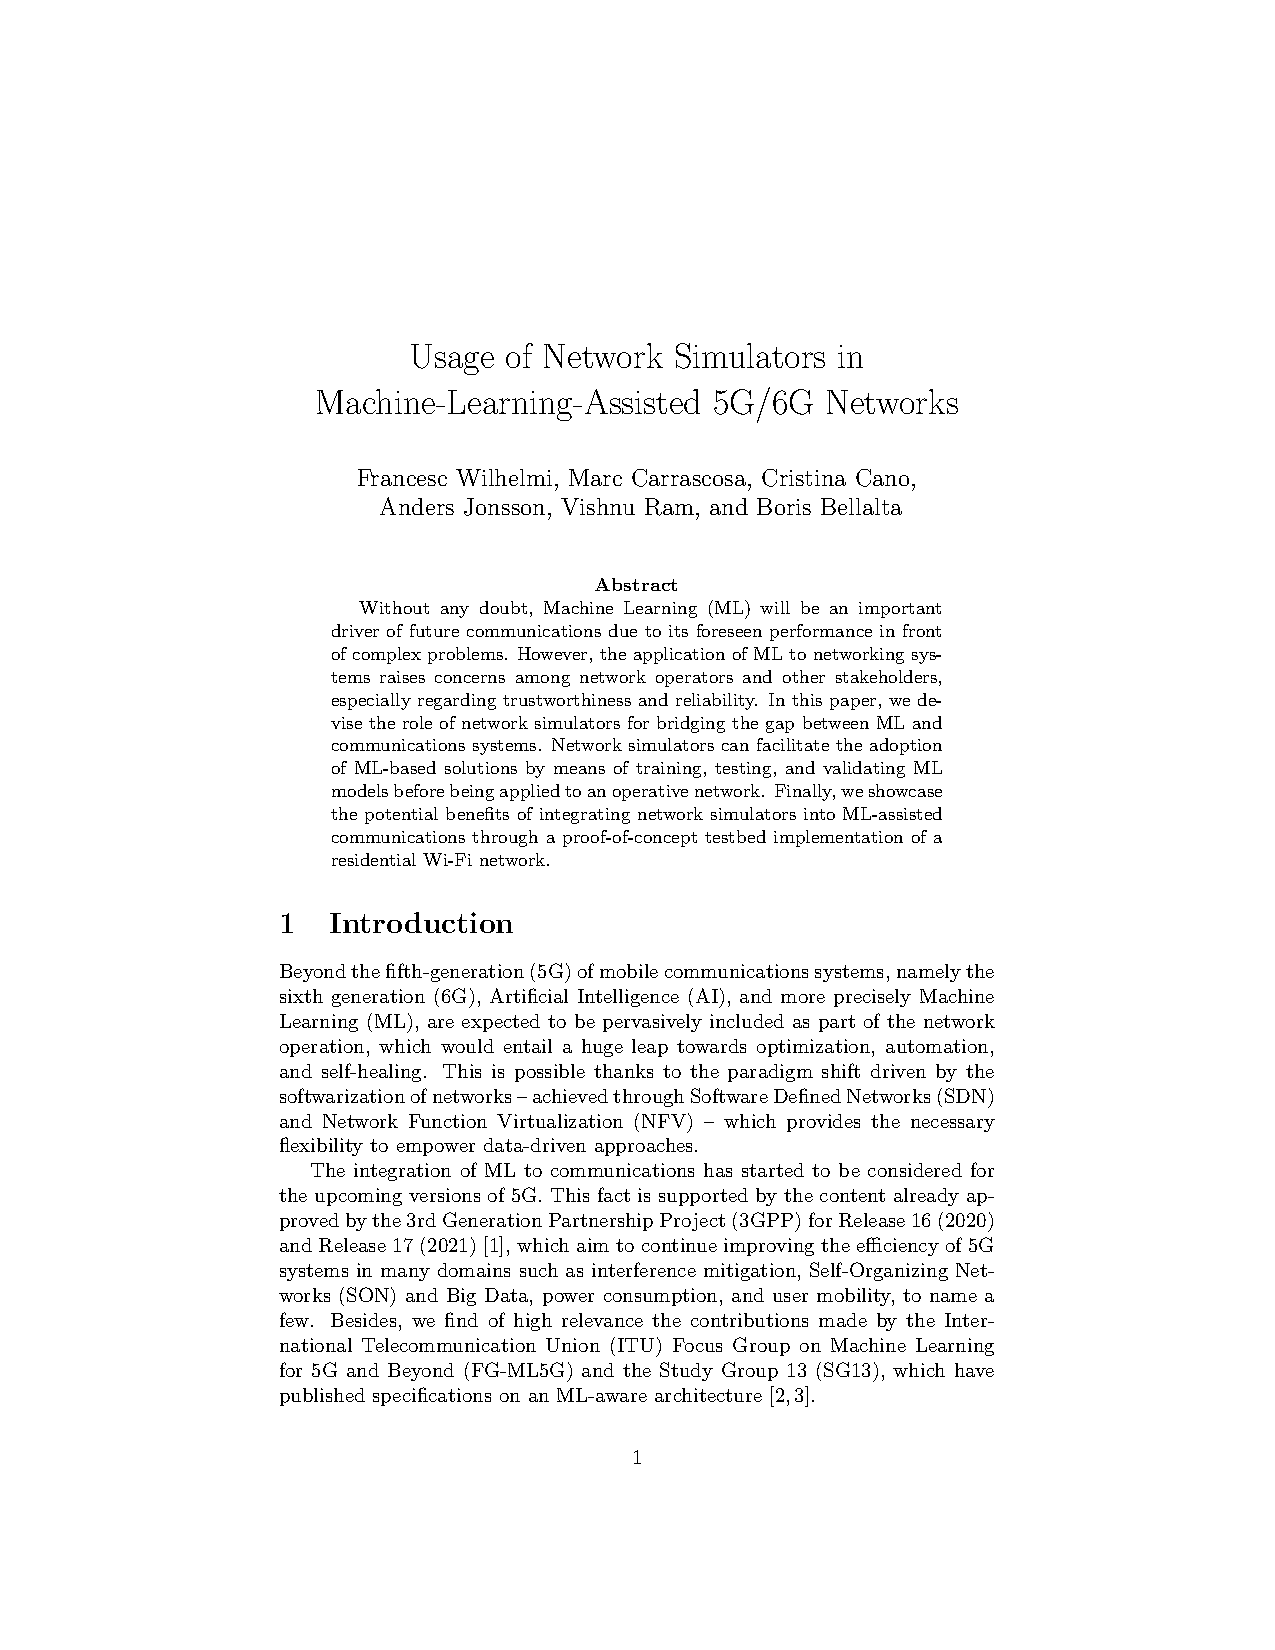
\includepdf[pages=1-]{papers/paper8/paper8.pdf}

\backmatter
\printindex

\end{document}

%NUMBER OF THE EXTERNAL PAGE EXCEPT IN THE FIRST PAGE OF EACH CAPITAL
\usepackage{fancyhdr}
\pagestyle{fancy}
\fancyfoot{}
\fancyfoot[RO]{\thepage}
\fancyfoot[LE]{\thepage}

%MULTIPLE INDEX
%In the preamble
\usepackage{multind}
\makeindex{authors}
%Introduction to form entries
%\index{authors}{Einstein}
%Situation of the Index
%\printindex{authors}{Author index}
%The \ usepakage {makeidx} \ makeindex \ printindex commands must be removed
%You need to execute from the command line makeindex authors